% ******************* PhD Thesis Presentation Template *************************
% Please have a look at the README.md file for info on how to use the template
\PassOptionsToPackage{table}{xcolor} % <-μονο εδω δουλεύει!!

\documentclass[aspectratio=169, printbib]{Classes/beamerPub}%%  
% ******************************************************************************
% ******************************* Class Options ********************************
% *********************** See README for more details **************************
% ******************************************************************************
%
% `aspectratio=169`: reduce ratio to 16:9
%
% `customfont`: Pre-defined font is "Biolinum O". This option enable custom fonts .
% Config custom fonts at `preamble.tex`. Custom font include GFS package.
%
% `10pt` or `11pt`(default) : Recommended font size. Smaller (`8pt`,`9pt`)
% or huge (`14pt`,`17pt`,`20pt`) font size are NOT recommended except special cases.
%
% `draft`: Special draft mode with line numbers, images, and water mark with 
% timestamp and custom text. Position of the text can also be modified. To 
% disable figures see on `preample.tex` the Draftmode section.
%
% `chapter`: This option enables only the specified chapter and it's references
% Useful for review and corrections.
%
% `notes`: Prints frames and notes 
%
% `notes=only`: Prints only notes of each frame
%
% `printbib`: Include bibliography at the end of the presentation 
%
% `progrbar`: Enable progress bar in the frame. Chose this option after your 
% first compilation. Disable on chapter mode.

% ********************************** Preamble **********************************
% Preamble: Contains packages and user-defined commands and settings
% ********************************** Preamble **********************************
% Preamble: Contains packages and user-defined commands and settings
%%-----------------------------------------------------------------------------
%% USE THEME
%%-----------------------------------------------------------------------------
\usetheme{BluePub}
% \usetheme{PaloAlto} 
% \usetheme{Singapore}
% \usetheme{Szeged}
% \usetheme{CambridgeUS}
% \usetheme{Montpellier}
% \usetheme{Pittsburgh} <---
% \usetheme{Warsaw}
% \usetheme{Rochester}
% \usetheme{Marburg}
% \usetheme{Malmoe}
% \usetheme{Madrid}
% \usetheme{Luebeck}
% \usetheme{Ilmenau}
% \usetheme{Hannover} <---
% \usetheme{Goettingen}
% \usetheme{Dresden}
% \usetheme{boxes}
% \usetheme{Boadilla}
% \usetheme{Berlin}
% \usetheme{Berkeley}
% \usetheme{AnnArbor}

\usepackage{lmodern}
\usepackage[scale=2]{ccicons}

%%-----------------------------------------------------------------------------
%%  remove dots from miniframe theme
%%-----------------------------------------------------------------------------
\makeatletter
\def\beamer@writeslidentry{\clearpage\beamer@notesactions}
\makeatother

%%-----------------------------------------------------------------------------
%%  double slides left presentation // right notes NOT WORK WELL!!!
%%-----------------------------------------------------------------------------
% \usepackage{pgfpages}
% \setbeameroption{show notes on second screen=right}

%%-----------------------------------------------------------------------------
%%  margins
%%-----------------------------------------------------------------------------
\setbeamersize{text margin left=0.4cm}  % <- like this
\setbeamersize{text margin right=0.4cm} % <- like this

%%-----------------------------------------------------------------------------
%% Set background for simpledso theme
%%-----------------------------------------------------------------------------
%\graphicspath{{Chapter3/Figs/Vector/}{Chapter3/Figs/}}
\setwatermark{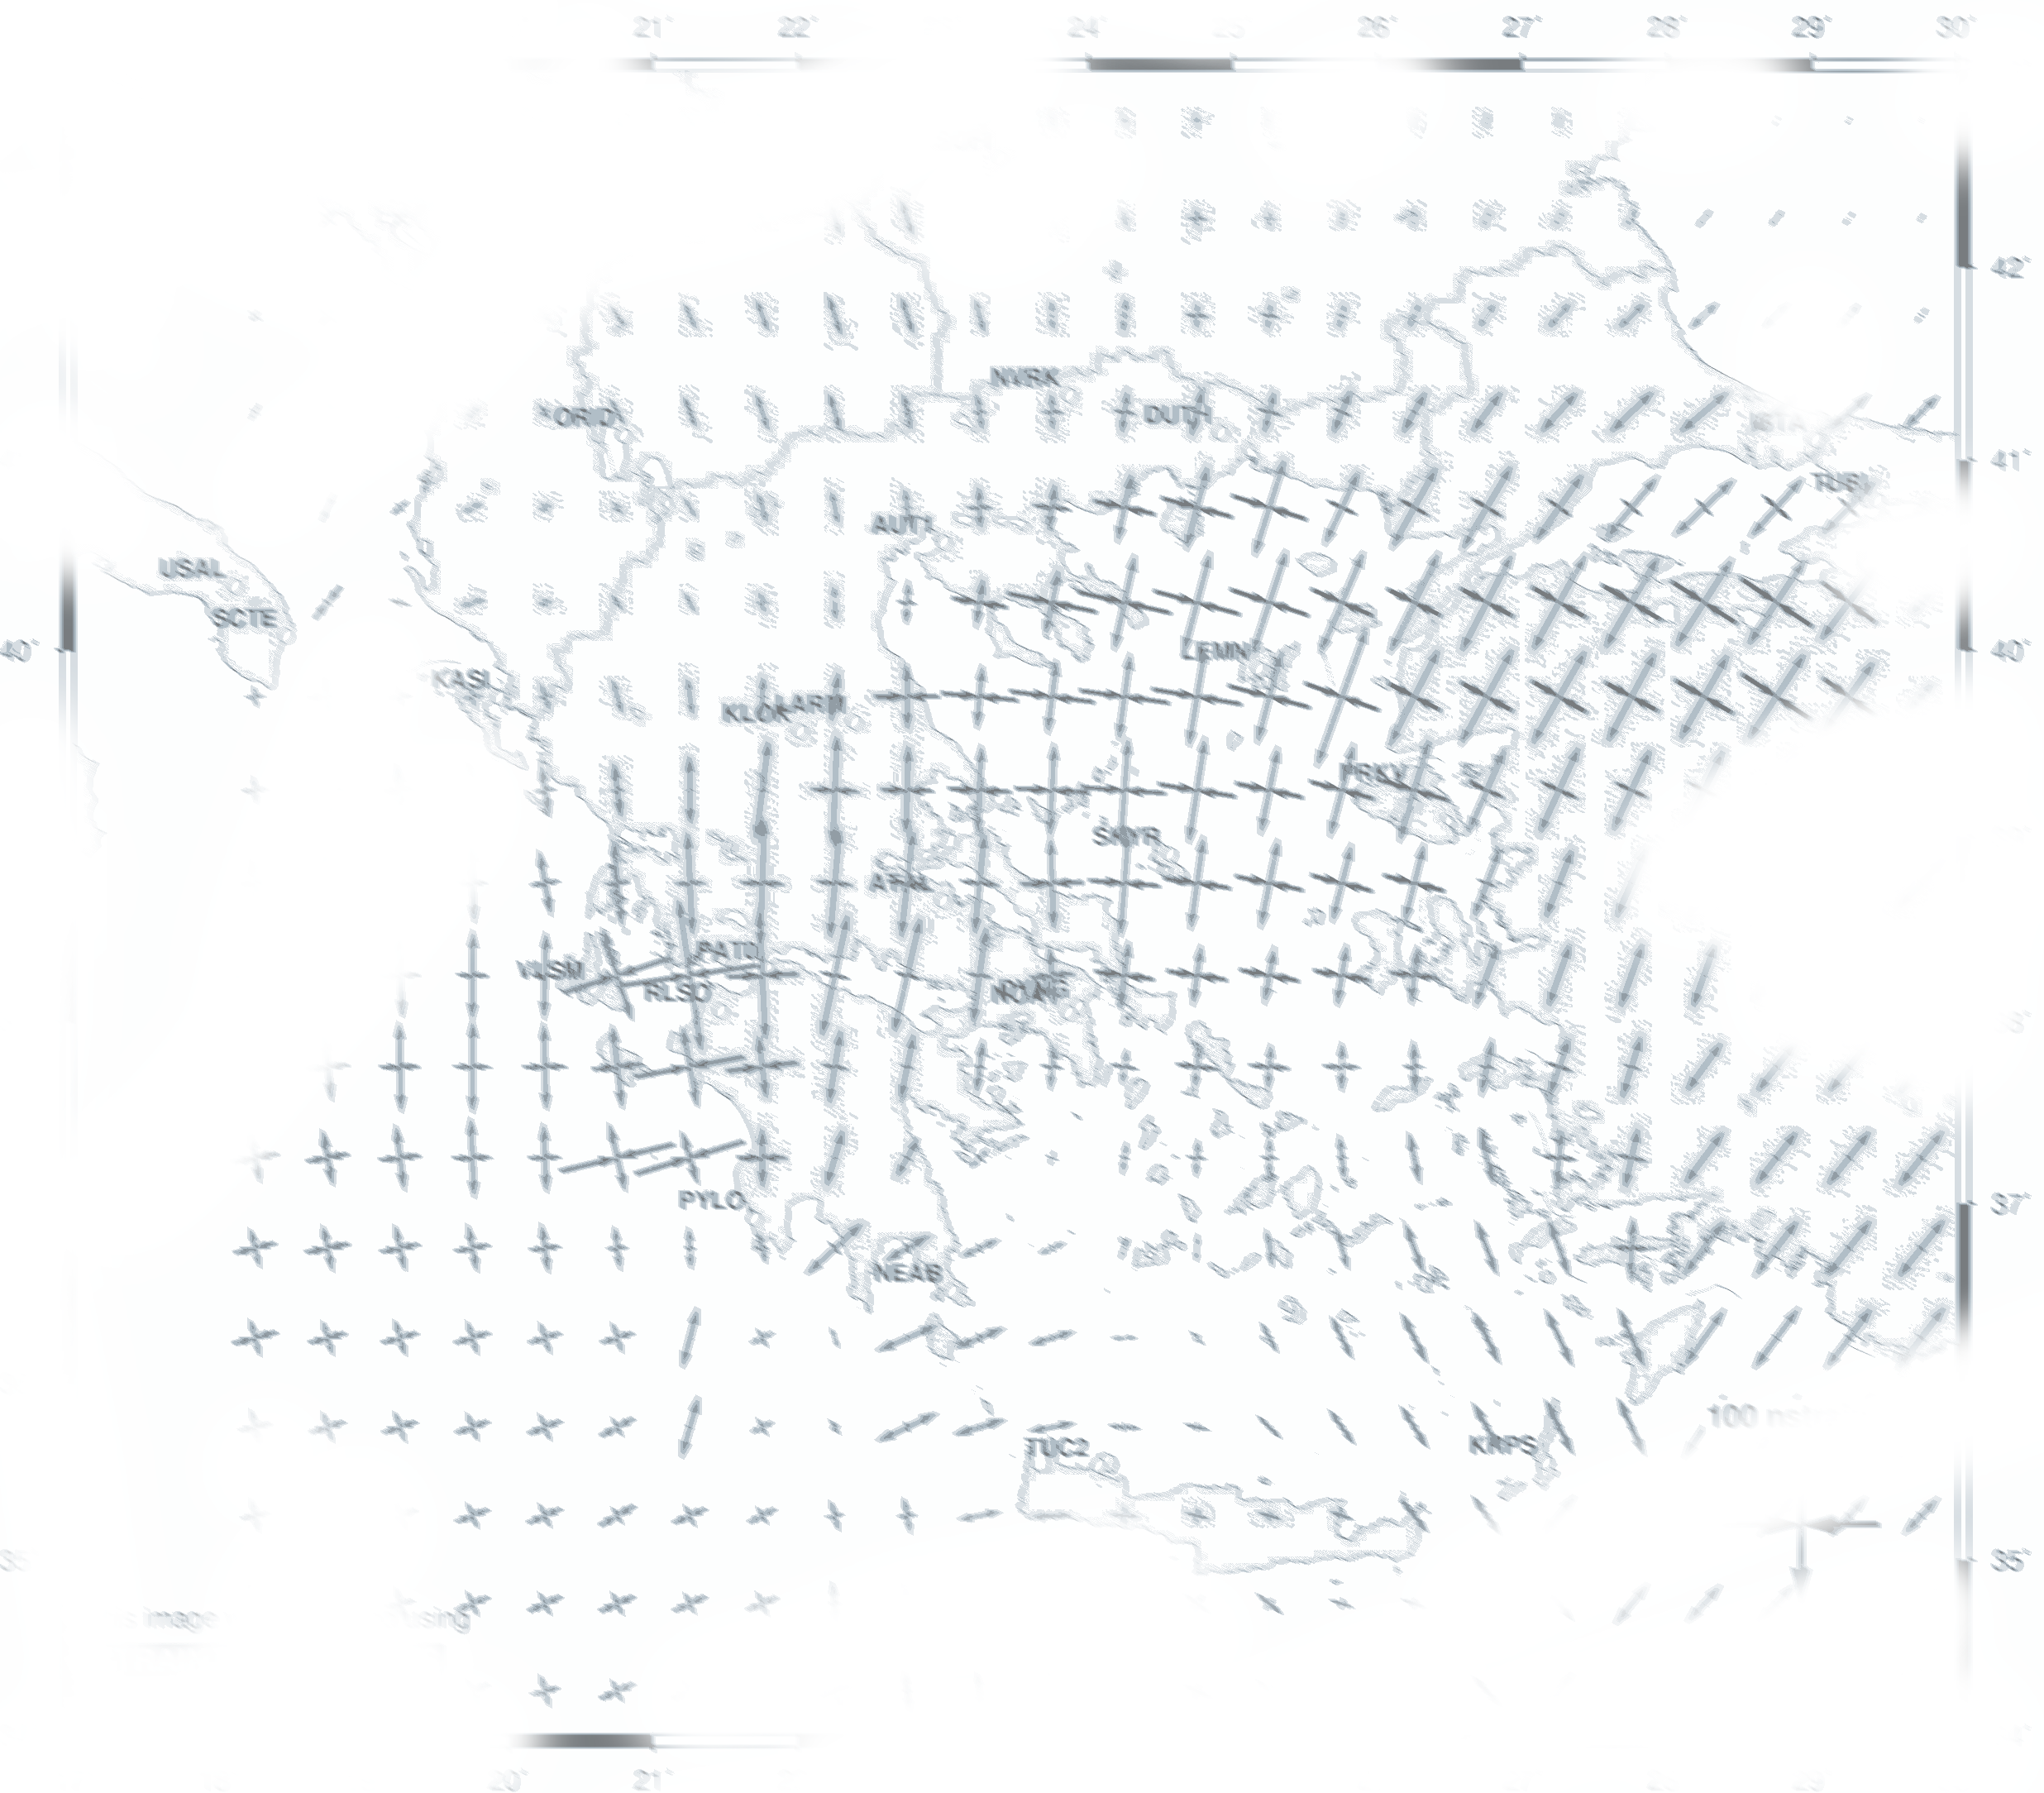
\includegraphics[height=8cm,draft=false]{Figs/back_str.png}}

%%-----------------------------------------------------------------------------
%% Languages
%%-----------------------------------------------------------------------------
% \usepackage[english, greek]{babel}
\usepackage{xgreek}
\usepackage[Greek,Latin]{ucharclasses}
\setTransitionsForGreek{\setlanguage{greek}}{\setlanguage{english}}
% \usepackage{xunicode}
% \usepackage{xltxtra}
% \usepackage[monogreek]{xgreek}
% \usepackage{tabu}

%%-----------------------------------------------------------------------------
%% Tables
%%-----------------------------------------------------------------------------
\usepackage{booktabs,tabularx}
\usepackage{tabu}
\usepackage{multirow}

%%-----------------------------------------------------------------------------
%% Fonts
%%-----------------------------------------------------------------------------

% Add `customfont' in the document class option to use this section
\ifdefineCustomFont
  \usepackage{fontspec}
  \usefonttheme{professionalfonts} % using non standard fonts for beamer
  \usefonttheme{serif} % default family is serif
%  \setmainfont[Mapping=tex-text]{GFS Didot}
%  \setmainfont[Mapping=tex-text]{GFS Bodoni}
%  \setmainfont[Mapping=tex-text]{GFS Olga} % ότι να ναι αυτή!!πλάγια NOT support English
  \setmainfont[Mapping=tex-text]{GFS Neohellenic}
%  \setmainfont[Mapping=tex-text]{GFS Artemisia}
%  \setmainfont[Mapping=tex-text]{GFS Elpis} %low resolution printing


%%  % For use with XeLaTeX, enable Libertine
%    \setmainfont[
%      Path              = /usr/share/texlive/texmf-dist/fonts/opentype/public/libertine/, %./libertine/opentype/,
%      Extension         = .otf,
%      UprightFont = LinLibertine_R,
%      BoldFont = LinLibertine_RZ, % Linux Libertine O Regular Semibold
%      ItalicFont = LinLibertine_RI,
%      BoldItalicFont = LinLibertine_RZI, % Linux Libertine O Regular Semibold Italic
%    ]
%    {LGR}
%  %  % load font from system font
%     \newfontfamily\libertinesystemfont{Linux Libertine O}

%  %% use xetex, enable Biolinum Fonts
%  \setmainfont[
%      Path              = /usr/share/texlive/texmf-dist/fonts/opentype/public/libertine/, %./libertine/opentype/,
%      Extension         = .otf,
%      UprightFont = LinBiolinum_R,
%      BoldFont = LinBiolinum_RB, % Linux Libertine O Regular Semibold
%      ItalicFont = LinBiolinum_RI,
%      %BoldItalicFont = LinBiolinum_RZI, % Linux Libertine O Regular Semibold Italic
%    ]
%    {LGR}
%  %  % load font from system font
%     \newfontfamily\libertinesystemfont{Linux Biolinum O}


\else
  \usepackage{fontspec}
  \usefonttheme{professionalfonts} % using non standard fonts for beamer
  \usefonttheme{serif} % default family is serif

  %% Use Computer Modern Unicode Fonts, Support Greek Font
  \setmainfont[Mapping=tex-text, Scale=0.90]{CMU Serif}
  \setsansfont[Mapping=tex-text, Scale=0.90]{CMU Sans Serif}
  \setmonofont{CMU Typewriter Text}
 
%%************* Latin Modern, not support greek*****************************
%  \usepackage{lmodern}
%  \usepackage[T1]{fontenc}
     
\fi % custom font class

%%-----------------------------------------------------------------------------
%% REQUIRED PACKAGES
%%-----------------------------------------------------------------------------
\usepackage{graphicx}  % Required for including images
\usepackage{fancybox}
% \usepackage{xcolor}
%% for tikz
% \usepackage{dtklogos}
%\usepackage{tikz}
\usetikzlibrary{mindmap,shadows}
\usepackage{smartdiagram}

% restart numbering footnotes per page
\usepackage{perpage}
\MakePerPage{footnote}
% % Sychronize footnotes on columns minipages
\renewcommand\thempfootnote{\arabic{mpfootnote}}

% use nice itemlists ..
%\usepackage{enumitem, color, amssymb}
\usepackage{url}
% \hypersetup{colorlinks,linkcolor=,urlcolor=links}
\hypersetup{colorlinks=true,allcolors=blue}

% use metalogo to print xelatex!
\usepackage{metalogo}

% % tcolorbox custom block, problem with caption package, cant solve it yet!
% \usepackage[most]{tcolorbox}

%%-----------------------------------------------------------------------------
%% Adgust figures
%%-----------------------------------------------------------------------------
\usepackage{adjustbox} % for \adjincludegraphics
% {\shadowbox{\color{black!35}\includegraphics[height=4cm]{img/iono.eps}}

%%-----------------------------------------------------------------------------
%% Print Arrows
%%-----------------------------------------------------------------------------
\usepackage{marvosym} % \MVRIGHTarrow
\usepackage{stmaryrd} % \shortrightarrow $\Rightarrow$
\usepackage{textcomp} % \textrightarrow

%%-----------------------------------------------------------------------------
%% Math symbols
%%-----------------------------------------------------------------------------
\usepackage{amssymb} 
\usepackage{amsmath}

% \usepackage{soul}
% \definecolor{lightblue}{rgb}{.90,.95,1}
% \sethlcolor{lightblue}
% \renewcommand<>{\hl}[1]{\only#2{\beameroriginal{\hl}}{#1}}
% -----------------------------------------------------------------------------
% CAPTIONS
%-----------------------------------------------------------------------------
\usepackage{caption}
\usepackage{subcaption}
\captionsetup[figure]{font=footnotesize,labelfont=footnotesize,skip=0pt,belowskip=0pt}
\setbeamertemplate{caption}[numbered]

\setbeamerfont{caption}{size=\scriptsize}

% -----------------------------------------------------------------------------
% Four Quad
%-----------------------------------------------------------------------------
\newcommand\FourQuad[4]{
    \begin{minipage}[b][.45\textheight][t]{.50\textwidth}\centering#1\end{minipage}\hfill%
    \begin{minipage}[b][.45\textheight][t]{.50\textwidth}\centering#2\end{minipage}\\[0.1cm]
    \begin{minipage}[b][.45\textheight][t]{.50\textwidth}\centering#3\end{minipage}\hfill
    \begin{minipage}[b][.45\textheight][t]{.50\textwidth}\centering#4\end{minipage}%
}

% -----------------------------------------------------------------------------
% Custom symbols for itemize
%-----------------------------------------------------------------------------

\newenvironment{proenv}{\only{\setbeamercolor{local structure}{fg=green}}}{}
\newenvironment{conenv}{\only{\setbeamercolor{local structure}{fg=red}}}{}
 \usepackage{fontawesome}

% -----------------------------------------------------------------------------
% Rotate text
%-----------------------------------------------------------------------------
\usepackage{rotating}
%\begin{turn}{45} 
% ...
% \end{turn}


% -----------------------------------------------------------------------------
% BIBLATEX
%-----------------------------------------------------------------------------
\usepackage{hyperref}
\usepackage[backend=biber,
            style=authoryear,
            maxbibnames=9,
            maxcitenames=1,
            citestyle=authoryear,
            hyperref=true,
            backref=true,
            sorting=nty,
            natbib=true]{biblatex}

% Hypper linc for all citations use \parencite & \textcite
\ExecuteBibliographyOptions{maxcitenames=1}

\DeclareFieldFormat{citehyperref}{%
  \DeclareFieldAlias{bibhyperref}{noformat}% Avoid nested links
  \bibhyperref{#1}}

\DeclareFieldFormat{textcitehyperref}{%
  \DeclareFieldAlias{bibhyperref}{noformat}% Avoid nested links
  \bibhyperref{%
    #1%
    \ifbool{cbx:parens}
      {\bibcloseparen\global\boolfalse{cbx:parens}}
      {}}}

\savebibmacro{cite}
\savebibmacro{textcite}

\renewbibmacro*{cite}{%
  \printtext[citehyperref]{%
    \restorebibmacro{cite}%
    \usebibmacro{cite}}}

\renewbibmacro*{textcite}{%
  \ifboolexpr{
    ( not test {\iffieldundef{prenote}} and
      test {\ifnumequal{\value{citecount}}{1}} )
    or
    ( not test {\iffieldundef{postnote}} and
      test {\ifnumequal{\value{citecount}}{\value{citetotal}}} )
  }
    {\DeclareFieldAlias{textcitehyperref}{noformat}}
    {}%
  \printtext[textcitehyperref]{%
    \restorebibmacro{textcite}%
    \usebibmacro{textcite}}}



\bibliography{References/triangleref.bib}
\newcounter{bibitmctr}
\newcommand{\brf}{%
  \stepcounter{bibitmctr}%
  \ifnum\value{bibitmctr}=7%
    \setcounter{bibitmctr}{0}
    \framebreak
  \fi
}

\renewbibmacro*{finentry}{\finentry\brf}

% % cahnge fontsize of bibliography for biblatex
\renewcommand*{\bibfont}{\tiny}


%%-----------------------------------------------------------------------------
%% Insert frame after new section
%%-----------------------------------------------------------------------------
%%% comment next lines if you don't like to use this
%\AtBeginSection[]{
%  \begin{frame}[b]
%%   \vfill
%  \vspace{\fill}
%  \centering
%  \begin{beamercolorbox}[sep=8pt,center,shadow=true,rounded=true]{title}
%    \usebeamerfont{title}\Large{\insertsection} %
%  \end{beamercolorbox}
%  \vskip-2cm
%  \begin{flushleft}
%    {\color{red!20}\rule{0.7\textwidth}{1pt}}\par
%    {\color{red!40}\rule{0.5\textwidth}{1pt}}\par
%    {\color{red!60}\rule{0.3\textwidth}{1pt}}\par
%    {\color{red!70}\rule{0.16\textwidth}{1pt}}\par
%    {\color{red!80}\rule{0.08\textwidth}{1pt}}\par
%    {\color{red!90}\rule{0.04\textwidth}{1pt}}\par
%  \end{flushleft}
%  \vspace{.5cm}
%%   \vfill
%  \end{frame}
%}

% -----------------------------------------------------------------------------
% Configure Draft mode
%-----------------------------------------------------------------------------
% *********************** Configure Draft Mode **********************************
\ifsetDraft
  \usepackage[printwatermark]{xwatermark}
  % Bottom
  \newwatermark*[pages=2-,color=red!60,textalign=center,angle=0,scale=.37,xpos=-.2cm,ypos=-.437\paperheight]{\makebox[.9\textwidth]{{\drafttext}\space-\space{\draftVersion}\space{\timestamp}}}
  %Flush right
%  \newwatermark*[pages=2-,color=red!60,textalign=center,angle=90,scale=.35,xpos=.45\paperwidth, ypos=-.7cm]{\makebox[.9\textwidth]{{\drafttext}\space-\space{\draftVersion}\space{\timestamp}}}
  
\fi 

% Uncomment to disable figures in `draft' mode
% \setkeys{Gin}{draft=true}  % set draft to false to enable figures in `draft'

% These options are active only during the draft mode
% Default text is "Draft"
\SetDraftText{DRAFT}

% Draft Version - default is v1.0
\SetDraftVersion{v1.0}

% ******************************** Todo Notes **********************************
%% Uncomment the following lines to have todonotes. % Not working yet!

% \ifsetDraft
%   \usepackage[colorinlistoftodos,prependcaption,textsize=small]{todonotes}
%   \setlength{\marginparwidth}{2.2cm}
% % 	\usepackage[colorinlistoftodos]{todonotes}
% 	\newcommand{\mynote}[1]{\todo[author=mitsos,size=\small,inline,color=green!40]{#1}}
%   \newcommand{\unsure}[1]{\todo[author=mitsos,size=\small,color=red!60]{#1}}
% 	\newcommand{\change}[2][1=]{\todo[author=mitsos,size=\small,linecolor=blue,backgroundcolor=blue!35,bordercolor=blue]{#1}}
% % 	\newcommand{\info}[2][1=]{\todo[linecolor=OliveGreen,backgroundcolor=OliveGreen!25,bordercolor=OliveGreen,#1]{#2}}
% % 	\newcommand{\improvement}[2][1=]{\todo[linecolor=Plum,backgroundcolor=Plum!25,bordercolor=Plum,#1]{#2}}
% 	\newcommand{\xanthos}[1]{\todo[author=xanthos,size=\small,inline,color=red!40]{#1}}
% 	\newcommand{\vagg}[1]{\todo[author=vagg,size=\small,inline,color=red!40]{#1}}
% \else
%   \newcommand{\todo}[1]{}
% 	\newcommand{\mynote}[1]{}
% 	\newcommand{\unsure}[1]{}
% 	\newcommand{\change}[1]{}
% 	\newcommand{\info}[2][1=]{}
% 	\newcommand{\improvement}[2][1=]{}
% 	\newcommand{\xanthos}[1]{}
% 	\newcommand{\vagg}[1]{}
% 	\newcommand{\listoftodos}{}
% \fi
%
% Example todo: \mynote{Hey! I have a note}


% ************************ Thesis Information & Meta-data **********************
% Thesis title and author information, refernce file for biblatex
% ************************ Pres Information & Meta-data ************************
% This file includes all available informations and meta-data for your presentation
% in four sections:
% 1. General & contact informations, for all styles.
% 2. PhD: Use this section with PhD style.
% 3. Pub: Use this section with publication style.
% 4. Lct: Usethis section with lecture style.
%
% Uncomment only one section of 2,3 or 4 each time.

%% -----------------------------------------------------------------------------
%% 1.General information... 
%% -----------------------------------------------------------------------------
% ************************ Pres Information & Meta-data ************************

%% Meta information
% \subject{Γεωδαισία} \keywords{{Γεωδαισία} {Τριγωνισμός} {Παραμόρφωση} {Ελλάδα}}

%% Contact e-informations
\urlhome{http://dionysos.survey.ntua.gr/}  %% homepage
\contmail{danastasiou@mail.ntua.gr}  %% contact mail
\urlin{https://www.linkedin.com/in/dganastasiou/}  %% linkedin url
\urlgh{https://github.com/demanasta}  %% github repository
%\urlgp{https://plus.google.com/u/0/+DemitrisAnastasiou}  %% Google+ 
\urltw{https://twitter.com/DemAnast}  %% Twitter

%% Add "thank you" text% 
\thankutext{Ευχαριστούμε για την προσοχή σας!}

% %% -----------------------------------------------------------------------------
% %% 2.PhD section INFO
% %% -----------------------------------------------------------------------------
% %% ************************ Thesis Information & Meta-data **********************
% %% The title of the thesis
% \eltitle{ΠΡΟΤΥΠΟ ΠΑΡΟΥΣΙΑΣΗΣ ΣΕ ΠΑΡΙΒΑΛΛΟΝ \\ Beamer-\LaTeX / \XeLaTeX}
% 
% %% Subtitle (Optional)
% % \subtitle{Using the CUED template}
% 
% %% The full name of the author
% \authorname{ΔΗΜΗΤΡΙΟΣ Γ. ΑΝΑΣΤΑΣΙΟΥ}
% \authortitle{Διπλ. Αγρονόμος \& Τοπογράφος Μηχανικός Ε.Μ.Π}
% 
% %% Department (eg. Department of Engineering, Maths, Physics)
% \dept{ΣΧΟΛΗ ΑΓΡΟΝΟΜΩΝ \& ΤΟΠΟΓΡΑΦΩΝ ΜΗΧΑΝΙΚΩΝ}
% 
% %% Laboratory
% \lab{ΚΕΝΤΡΟ ΔΟΡΥΦΟΡΩΝ ΔΙΟΝΥΣΟΥ}
% 
% %% University and Crest
% \university{ΕΘΝΙΚΟ ΜΕΤΣΟΒΙΟ ΠΟΛΥΤΕΧΝΕΙΟ}
% 
% % Crest minimum should be 30mm.
% \crestleft{
\includegraphics[width=\textwidth,draft=false]{Figs/ntua.png}}
% \crestright{
\includegraphics[width=0.85\textwidth,draft=false]{Figs/DSOtrans.png}}
% 
% %% Full title of the Degree
% \degreetitle{ΔΙΔΑΚΤΟΡΙΚΗ ΔΙΑΤΡΙΒΗ}
% 
% % Supervisor
% \supervisor{......O/E.........\\ ....Θέση..........}
% 
% %% College affiliation (optional)
% \city{ΑΘΗΝΑ}
% 
% %% Submission date
% % Default is set as {\monthname[\the\month]\space\the\year}
% % \degreedate{\today} 
% \degreedate{5 Ιουλίου 2017}



%% -----------------------------------------------------------------------------
%% 3.Publication's section INFO
%% -----------------------------------------------------------------------------
%% The title of the thesis
\prestitle{Υποστήριξη του δικτύου μόνιμων σταθμών GNSS\\ του Ελληνικού Κτηματολογίου\\ Επεξεργασία δεδομένων - Ανάλυση χρονοσειρών θέσης}

%% The team prepare this presentation
\presteam{Μαρία Τσακίρη,
Ξάνθος Παπανικολάου,
Δημήτριος Αναστασίου}

%% Organizations of the team
\presorgn{Κέντρο Δορυφόρων Διονύσου\\ Σχολή Αγρονόμων και Τροπογράφων Μηχανικών - Μηχανικών Γεωπληροφορικής \\ Εθνικό Μετσόβιο Πολυτεχνείο\\
}
%Contact informations
\presweb{dionysos.survey.ntua.gr}  % webpage
\presmail{dso@survey.ntua.gr}  % contact mail

%% Conference details, Select  text or logo type. If you define both only logo will
%% be print
% \confname{12\textsuperscript{th} HSTAM International Congress on Mechanics}
% \confdetail{Thessaloniki, Greece, 22 - 25 September 2019}

%% OR conf logo....
\conflogo{
\begin{minipage}{5cm}
\begin{flushright}
\vskip-1cm
\textit{Διαδικτυακή παρουσίαση}\\
\textbf{Τετάρτη 14 Ιουνίου}\\
\textbf{2023}
\end{flushright}
\end{minipage}

\includegraphics[width=3cm,draft=false]{Figs/ktima_logo.png}}

%% -----------------------------------------------------------------------------
%% 4.Course section INFO
%% -----------------------------------------------------------------------------
% 
% %%% Department (eg. Department of Engineering, Maths, Physics)
% \dept{ΣΧΟΛΗ ΑΓΡΟΝΟΜΩΝ \& ΤΟΠΟΓΡΑΦΩΝ ΜΗΧΑΝΙΚΩΝ}
% 
% %% Laboratory
% \lab{ΚΕΝΤΡΟ ΔΟΡΥΦΟΡΩΝ ΔΙΟΝΥΣΟΥ}
% 
% %% University and Crest
% \university{ΕΘΝΙΚΟ ΜΕΤΣΟΒΙΟ ΠΟΛΥΤΕΧΝΕΙΟ}
% 
% % Crest minimum should be 30mm.
% \crestleft{
\includegraphics[width=\textwidth,draft=false]{Figs/ntua.png}}
% \crestright{
\includegraphics[width=0.85\textwidth,draft=false]{Figs/DSOtrans.png}}
% 
% 
% %% The full name of the author
% \authorname{ΔΗΜΗΤΡΙΟΣ Γ. ΑΝΑΣΤΑΣΙΟΥ}
% \authortitle{Δρ. Αγρ. \& Τοπ. Μηχ. Ε.Μ.Π}
% 
% %% Lecture title
% \coursetitle{Τίτλος του Μαθήματος}
% \courseinfo{5ο Εξάμηνο}
% \lcttitle{Δημιουργία παρουσιάσεων σε περιβάλλον {\LaTeX}}
% 
% 
% %%% College affiliation (optional)
% \city{ΑΘΗΝΑ}
% 
% %% Submission date
% % Default is set as {\monthname[\the\month]\space\the\year}
% % \degreedate{\today} 
% \coursedate{01 Οκτωβρίου 2017}












% ***************************** Chapter Mode ***********************************
\ifdefineChapter
\includeonly{Chapter1/ch1intro}
%\includeonly{Chapter2/ch2pres}
% \includeonly{Chapter3/ch3pres}
% \includeonly{Chapter4/ch4pres}
% \includeonly{Chapter5/ch5pres}
% \includeonly{Chapter6/ch6pres}
% \includeonly{Appendix/ap_refs}
% \includeonly{Appendix/ap_soft}
% \includeonly{Appendix/cut01.tex}
\fi

% ***********************  Start the document  ***********************************
\begin{document}

% *****************************  Make title  *************************************
\maketitle

% *****************************  TOC  *************************************
\begin{frame}
  \frametitle{Presentation Structure}
  \tableofcontents
\end{frame}


% ************************  Include Chapters  *************************************
\graphicspath{{Chapter1/Figs/}}

\section{Introduction}

\begin{frame}\frametitle{DSO Recent Activity}\framesubtitle{}
\vskip-1.5cm
  Dionysos Satellite Observatory (DSO) of the National Technical University of 
  Athens (NTUA), has developed and maintains an automated processing
  scheme to accommodate the routine analysis of all available continuous GNSS 
  stations in Greece.
  \\
  This daily analysis process is implemented for over five years now (not 
  always continuous though dues to various problems), yielding 
  results which help us further understand the complicated tectonic setting of 
  Greece and nearby regions.
  \\
  Important results, include:
  \begin{itemize}
    \item the recent volcanic activity in \emph{Santorini} (e.g. \cite{papoutsis}),
    \item the 2014 \emph{Kefallonia} earthquakes (e.g. \cite{sarkefalonia}, \cite{sakkas})
  \end{itemize}
\end{frame}
%
\begin{frame}\frametitle{Motivation}\framesubtitle{}
  % Via our contribution to EUREF and interaction with its community, we hope to:
  Routine GNSS processing and site/network monitoring is crucial, because:
  \begin{itemize}
    \item Greece lies in a region of utmost tectonic and volcanic unrest (e.g. 
      active volcano in Santorini isl.),
    \item results \& products are important to a series of fields spanning 
      the whole range of Geosciences,
    \item helps us follow and apply state-of-the-art technologies in GNSS analysis 
      \& Satellite Geodesy and expand \& modernize our research activity,
    \item contribute to the GNSS/EUREF community and be involved in ongoing/future projects,
    \item improve our academic services (NTUA is a University)
  \end{itemize}
  Throughout the last years, routine preocessing \& monitoring has hepled us gain 
  a more thorough view of the complex tectonic and volcanic setting of Greece.
\end{frame}

\section{GPS/GNSS Networks in Greece}

\begin{frame}\frametitle{The DataSet}\framesubtitle{}
\vskip-1.5cm
  %To contribute to the Densification we have to establish a credible dataset
  %(network). This has proven to be rather challenging !\\
  Routine processing for precise positioning, assumes a well establihed, 
  credible dataset (metadata). This has proven to be rather challenging! Lately, 
  the introduction of \texttt{M3G} has provided assistance.\\
  \bigskip
  Currently we process whatever we can get our hands on \ldots\\
  Problems:
  \begin{itemize}
    \item Inhomogenous dataset (\texttt{RINEX} of various versions, raw files, etc).
    \item Various maintainers, different mentalities.
    \item Different aquisition methods/rates.
    \item No log files for mainteners with no geodetic interest (e.g. surveying companies).
    \item Wide variety of equipment (not always included in \texttt{atx} files).
  \end{itemize}
\end{frame}
\note


\begin{frame}\frametitle{Network GREECE}\framesubtitle{}
\vskip-1.5cm

%Network installed/maintained by \texttt{COMET}\footnote{Center for Observation and Modeling of Earthquakes, \url{http://comet.nerc.ac.uk/}} \& \texttt{NTUA}.
\begin{columns}[T] % align columns
\begin{column}{.40\textwidth}
  Network \texttt{Greece} includes the majority of the available dataset (~100)
  but not all of them are (always/currently) active. Various providers but all 
  with geodetic interest \& ecquipment.

  {\small
  \begin{itemize}
    \setlength\itemsep{.1em}
    \item<pro@1-> covers all of Greece
    \item<pro@1-> different (geodetic type) equipment
    \item<pro@1-> credible time-span (early 2004 - now)
    \item<pro@1-> all free available GNSS data
    \item<con@1-> large data gaps \& inactive stations (?)
%    \item<con@1-> needs repairing
\end{itemize}
}
\end{column}%
\hfill%
\begin{column}{.60\textwidth}
 \begin{figure}
 \begin{center}
 \vskip -.2cm
 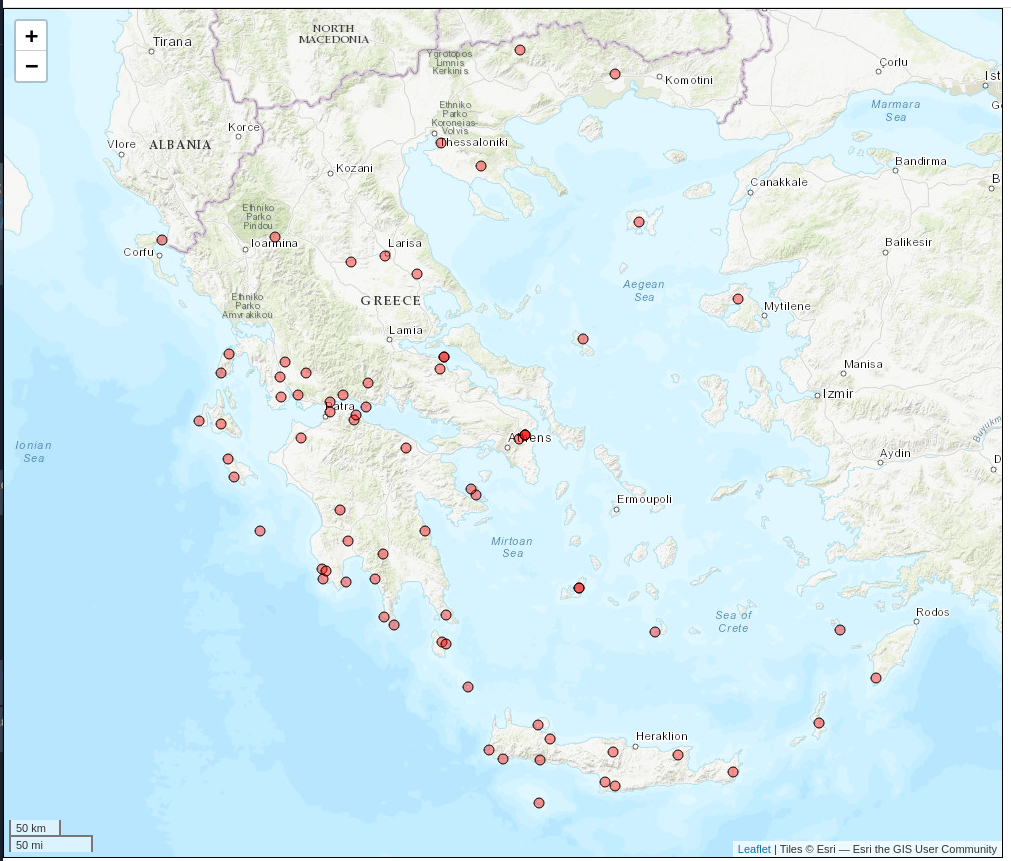
\includegraphics[width=.95\textwidth]{refag_greece_noref.png} %1 2.2 0 0
 \vskip .7cm
% \caption{COMET/NTUA network.}
\href{http://83.212.76.4/abmaps/netmap_noref.php?network=greece}{Network GREECE}
 \label{fig:cometntua}
 \end{center}
 \end{figure}
\end{column}%
\end{columns}
%  \begin{block}{}
%    Can be used for EUREF densification ``as is''.
%  \end{block}
\end{frame}


\begin{frame}\frametitle{Local Networks}\framesubtitle{}
\vskip-.7cm
  %Network installed/maintained by \texttt{CRLab}\footnote{Rift Laboratory \url{http://webobs.crlab.eu/}}. 
  the \texttt{Corinth Rift.} network is centered around the Cortinth Gulf, a 
  region of special tectonic interest. Larger site density compared to the 
  rest of Greece.
  \begin{itemize}
    \item<pro@1-> credible time-span
    \item<pro@1-> only covers the Corinth Rift
    \item<con@1-> different providers (including surveying \& cadastral services)
    \item<con@1-> no log files \& equipment changes
  \end{itemize}

 \begin{figure}
 \begin{center}
 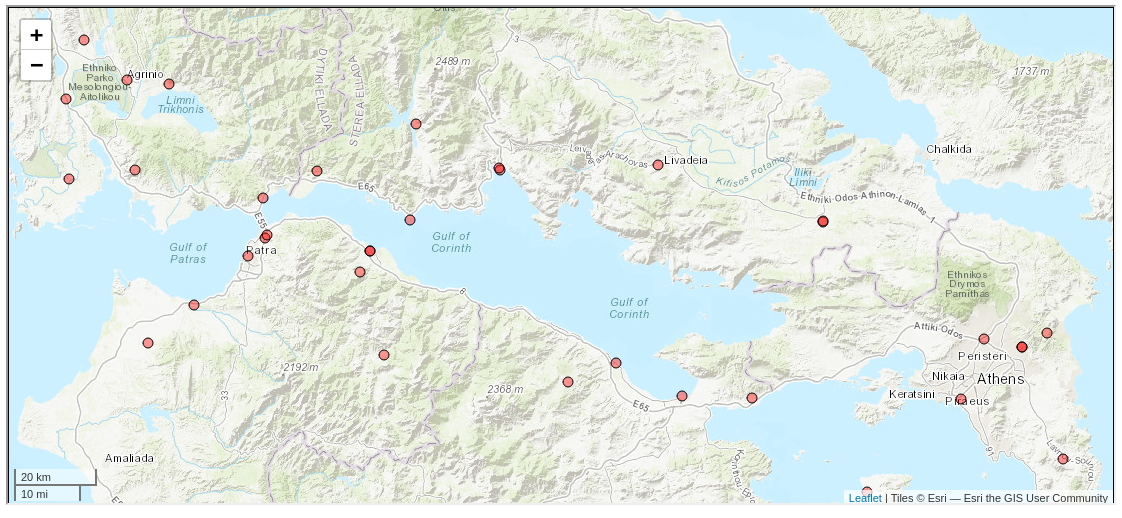
\includegraphics[trim={0cm 2.5cm 0cm 0cm},clip,width=.75\textwidth]{refag_crnet.png}
%  \vskip .6cm
% \caption{EnCeladus network. \url{http://dionysos.survey.ntua.gr/dso/enceladus/}}
  \url{http://dionysos.survey.ntua.gr/dso/enceladus/}
 \label{fig:crlab}
 \end{center}
 \end{figure}
%
%
%  \FourQuad
%  {
%  \textbf{Corinth Rift.}
%  \begin{itemize}
%    \item<pro@1-> credible time-span
%    \item<pro@1-> only covers the Corinth Rift
%    \item<con@1-> inconsistent providers
%    \item<con@1-> no log files \& equipment changes
%  \end{itemize}
%  }
%  {
%
%  }
%  {
%  \textbf{Santorini Network.}
%  Most of the stations installed post-2011 to monitor the \textit{inflation episode}.
%  \begin{itemize}
%    \item<con@1-> localized
%    \item<con@1-> limited time-span
%  \end{itemize}
%  }
%  {
% \begin{figure}
% \begin{center}
% 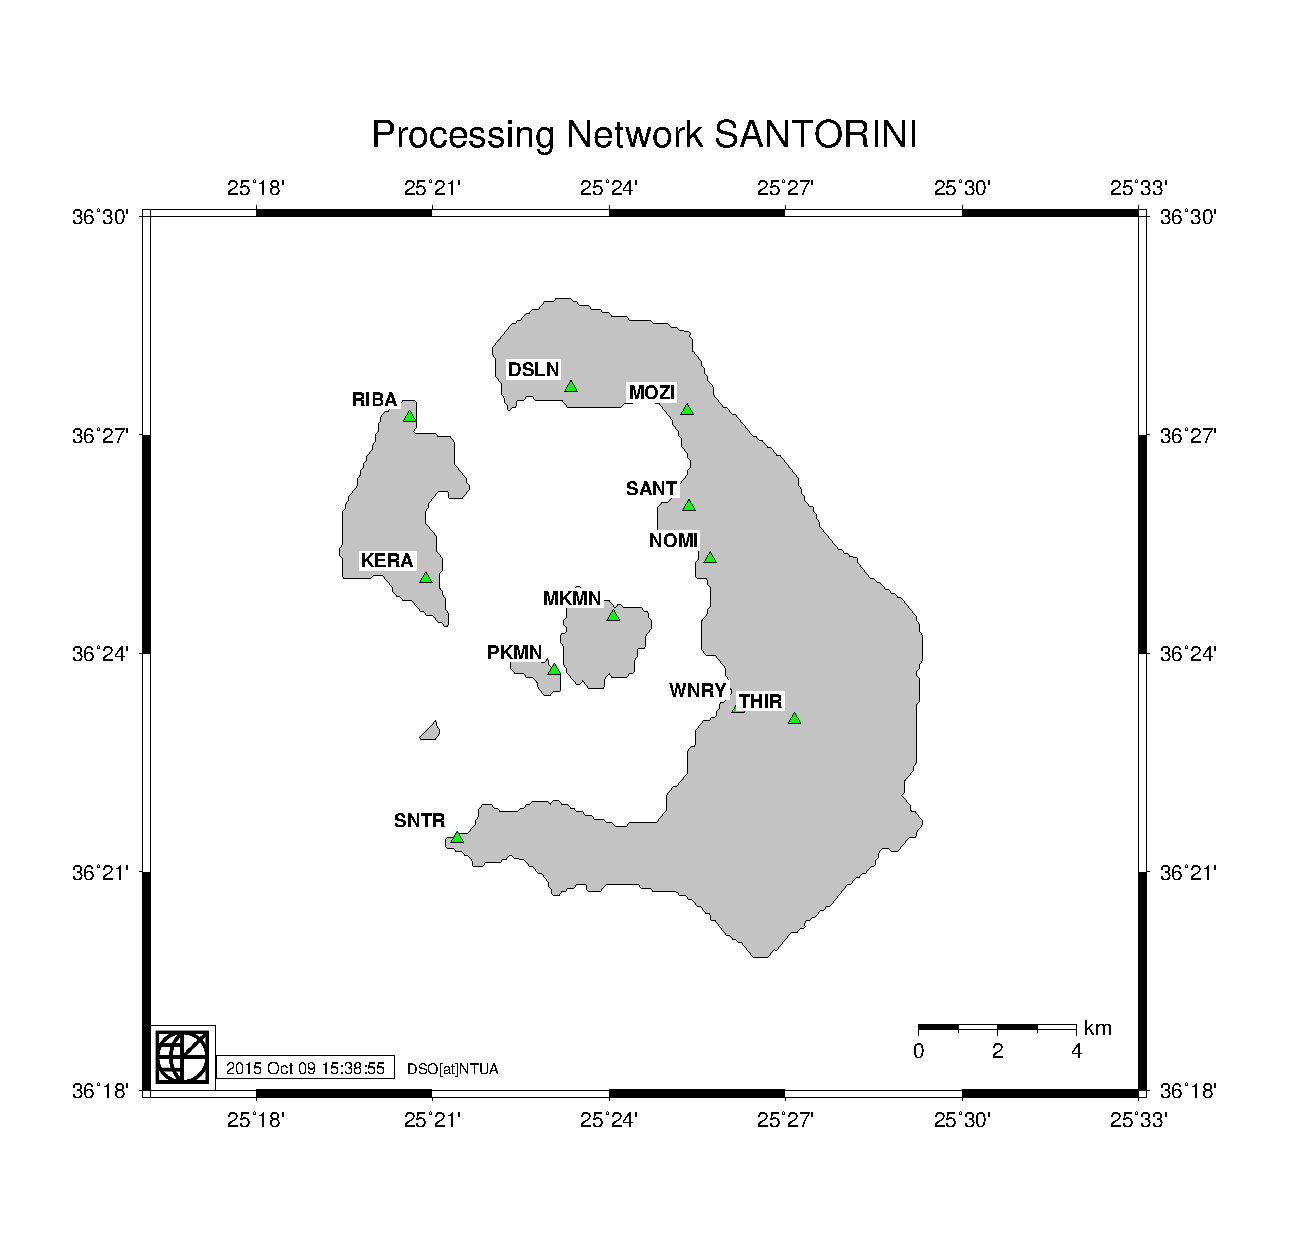
\includegraphics[trim={0cm 2.5cm 0cm 0cm},clip,width=.85\textwidth]{sntrnet.eps}
%  \vskip -.6cm
% \caption{Santorini network.}
% \label{fig:sntrnet}
% \end{center}
% \end{figure}
%  }


\end{frame}


\section{Processing}

\begin{frame}\frametitle{The Scheme}\framesubtitle{}
\begin{columns}[T] % align columns
\begin{column}{.35\textwidth}
   \footnotesize{The core tool/software is \texttt{Bernese GNSS Software v5.2}\cite{bpe}.\\
   %\medskip
   Integration with
   \begin{itemize}
    \setlength\itemsep{.5em}
     \item \textbf{MySQL} database,
     \item \textbf{Python} module (product/data downloading, pre-processing, 
      driving cron jobs, etc)
     \item \textbf{Time-series} analysis (integrated in routine processing on regular intervals)
     \item \textbf{Strain Rates} via StrainTool (on user demand)
   \end{itemize}}
\end{column}%
\hfill%

\begin{column}{.65\textwidth}
\vskip -1cm
\begin{figure}
\centering
   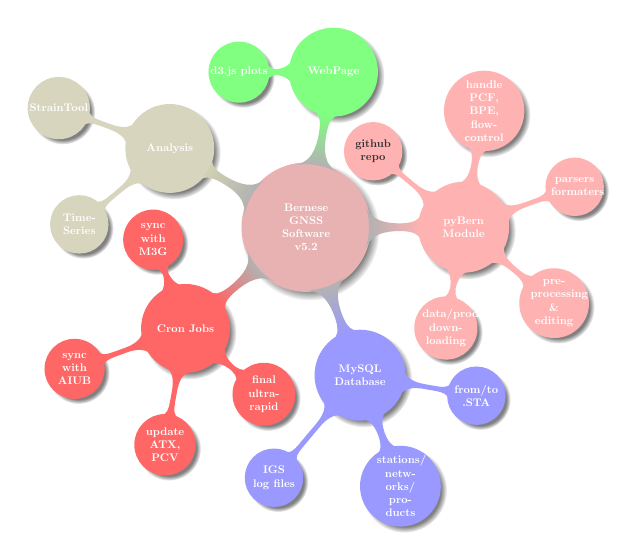
\begin{tikzpicture}[ every annotation/.style = {draw,
                      fill = white, font = \large}]

   \path[mindmap,concept color=black!30,text=white,
     every node/.style={concept,circular drop shadow, scale=.4},
     root/.style = {concept color=black!30!red!30,
font=\normalsize\bfseries,text width=5em},
     level 1 concept/.append style={
       font=\normalsize\bfseries, sibling angle=70,text width=7.7em,
       level distance=20mm,inner sep=0pt},
     level 2 concept/.append style={font=\bfseries,level distance=15mm},
   ]

   node[root] {Bernese GNSS Software v5.2} [clockwise from=0]
     child[concept color=red!30] {
       node {pyBern Module} [clockwise from=140]
       child  [color=black!80] { node {github repo} }
       child  { node {handle PCF, BPE, flow-control} }
       child  { node {parsers\\formaters} }
       child  { node {pre-processing \& editing} }
       child  [level distance=13mm] { node {data/product downloading} }
     }
     child[concept color=blue!40] {
       node[concept] {MySQL Database} [clockwise from=-10]
       child { node[concept] {from/to .STA} }
       child { node[concept] {stations/ networks/ products} }
       child [level distance=17mm] { node[concept] {IGS log files} }
     }
     child[concept color=red!60] {
       node[concept] {Cron Jobs} [clockwise from=-40]
       child [level distance=13mm] { node[concept] {final ultra-rapid} }
       child { node[concept] {update ATX, PCV } }
       child { node[concept] {sync with AIUB} }
       child [level distance=12mm, sibling angle=70] { node[concept]
{sync with M3G} }
     }
     child[concept color=yellow!40!black!30] {
       node[concept] { Analysis } [clockwise from=220]
       child { node[concept] {Time-Series} }
       child [text width=]{ node[concept] {StrainTool} }
     }
     child[concept color=green!50] {
       node[concept] { WebPage } [clockwise from=180]
       child [level distance=12mm, text width=] { node[concept] {d3.js
plots} }
     };
\end{tikzpicture}



\label{fig:software-design}
\end{figure}

\end{column}%
\end{columns}
\end{frame}

\begin{frame}\frametitle{Compliance wrt EUREF standards}\framesubtitle{}
\vskip-1.5cm
  Processing is consistent with EUREF standards (\href{http://www.epncb.oma.be/_documentation/guidelines/guidelines_analysis_centres.pdf}{Guidelines for Analysis Centres}).
  \begin{itemize}%%[label={\checkmark}]
    \item \texttt{SINEX} with required info/blocks,
    \item Reference frame \texttt{IGb14},
    \item \texttt{IERS} Conventions 2010,
    \item \texttt{IGS}/\texttt{CODE} products,
    \item ocean loading corrections (\texttt{FES2004}),
    %\item atmospheric tidal loading corrections,
    \item $3^{\circ}$ elevation cut-off angle; elevation dependent weighting,
    \item \texttt{GMF} and/or \texttt{VMF1}; \texttt{Chen-Herring} gradient parameter,
    \item amiguities fixed (length-dependent algorithm),
    \item use \texttt{GLONASS} obs (when available)
    \item ------------------ ATX/individual calibrations  -------------
  \end{itemize}
\end{frame}

%  \begin{itemize}
%    \item check station information file consistency (against the provided in \texttt{CODE}'s ftp)
%    \item synchronize \texttt{GEN/} directory
%    \item closely follow \texttt{RNX2SNX.PCF}
%    \begin{itemize}
%      \item variabes in PCF are set by external tools (genericity)
%      \item skip copying/moving/removing; replace with tools that interconnect with \texttt{MySQL}
%    \end{itemize}
%    \item update database
%    \item customize output (\texttt{html, json})
%  \end{itemize}
% \end{frame}

\begin{frame}\frametitle{Workflow}\framesubtitle{}
\begin{columns}[T] % align columns
\begin{column}{.48\textwidth}
  \texttt{\$>ddproces.sh --year= --doy= --session= --bern-loadgps= --campaign= --satellite-system= --solution-id= --save-dir= --analysis-center= --use-ntua-products= --append-suffix= --elevation-angle= --update= --pcv= --apply-exclude-list}
\end{column}
\hfill%
\begin{column}{.48\textwidth}
  \scalebox{0.5}{
  \smartdiagram[priority descriptive diagram]{
    Download \texttt{RINEX} consulting \texttt{MySQL} db,
    Download products,
    Validate \texttt{.STA}; synchronize \texttt{/GEN},
    Set variables in the Protocol Control File (\texttt{.PCF}),
    Process the dataset,
    Check for errors,
    Save Products \& Update database records,
    Compile Report (\texttt{json} | \texttt{html})
}}
\end{column}
\end{columns}
\end{frame}


\section{Results \& Outputs}

{
\usebackgroundtemplate{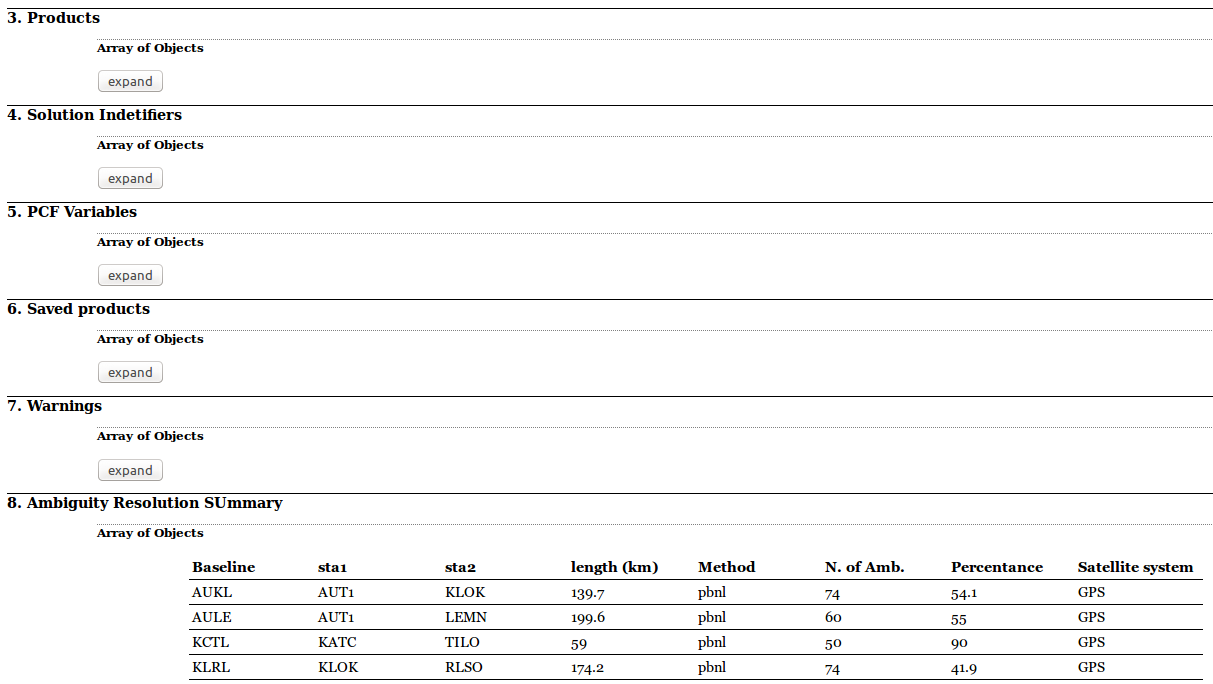
\includegraphics[height=.9\paperheight,width=.9\paperwidth]{jsonprint.png}}
\vskip-1.5cm
\begin{frame}\frametitle{Results \& Output}\framesubtitle{}
\begin{center}
\vskip -1.6cm
\begin{tikzpicture}
  \node (img1) {\shadowbox{\color{black!35}\includegraphics[height=4cm]{iono.eps}}};
%   \pause
  \node (img2) at (img1.north east) [yshift=-1cm,xshift=2.7cm] {\shadowbox{\color{black!35}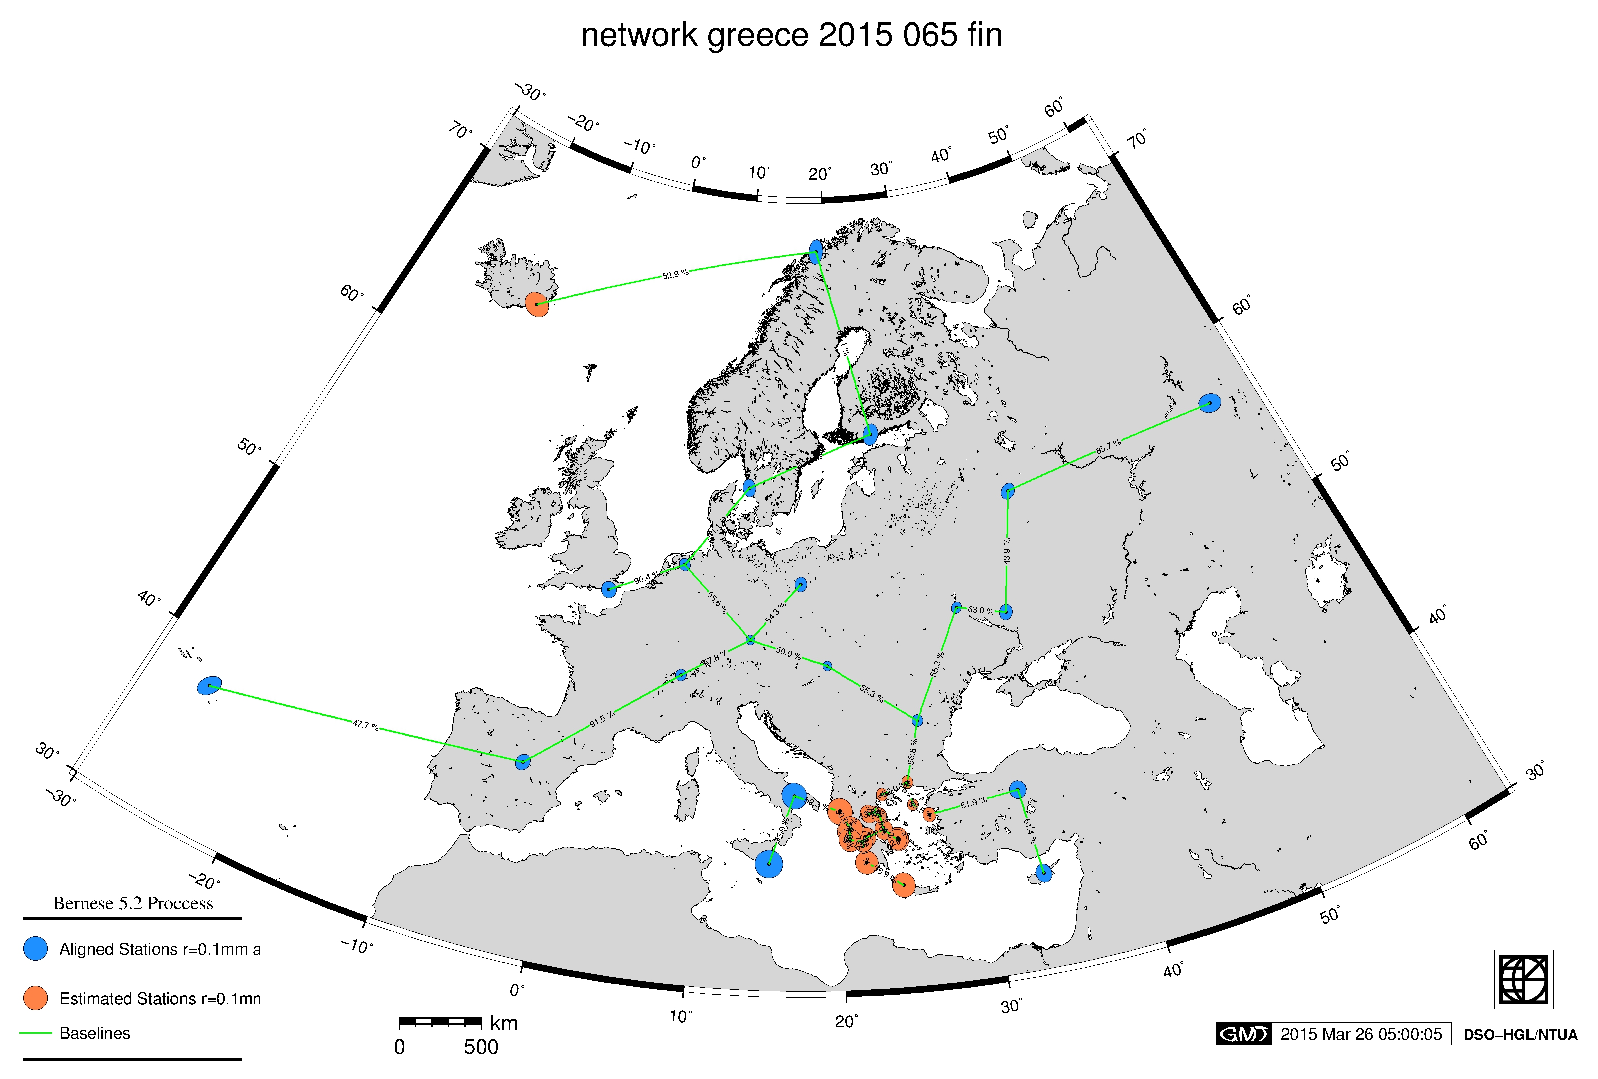
\includegraphics[height=2cm]{baseline.eps}}};
%   \pause
  \node (img3) at (img2.south) [yshift=-1.5cm,xshift=-.5cm] {\shadowbox{\color{black!35}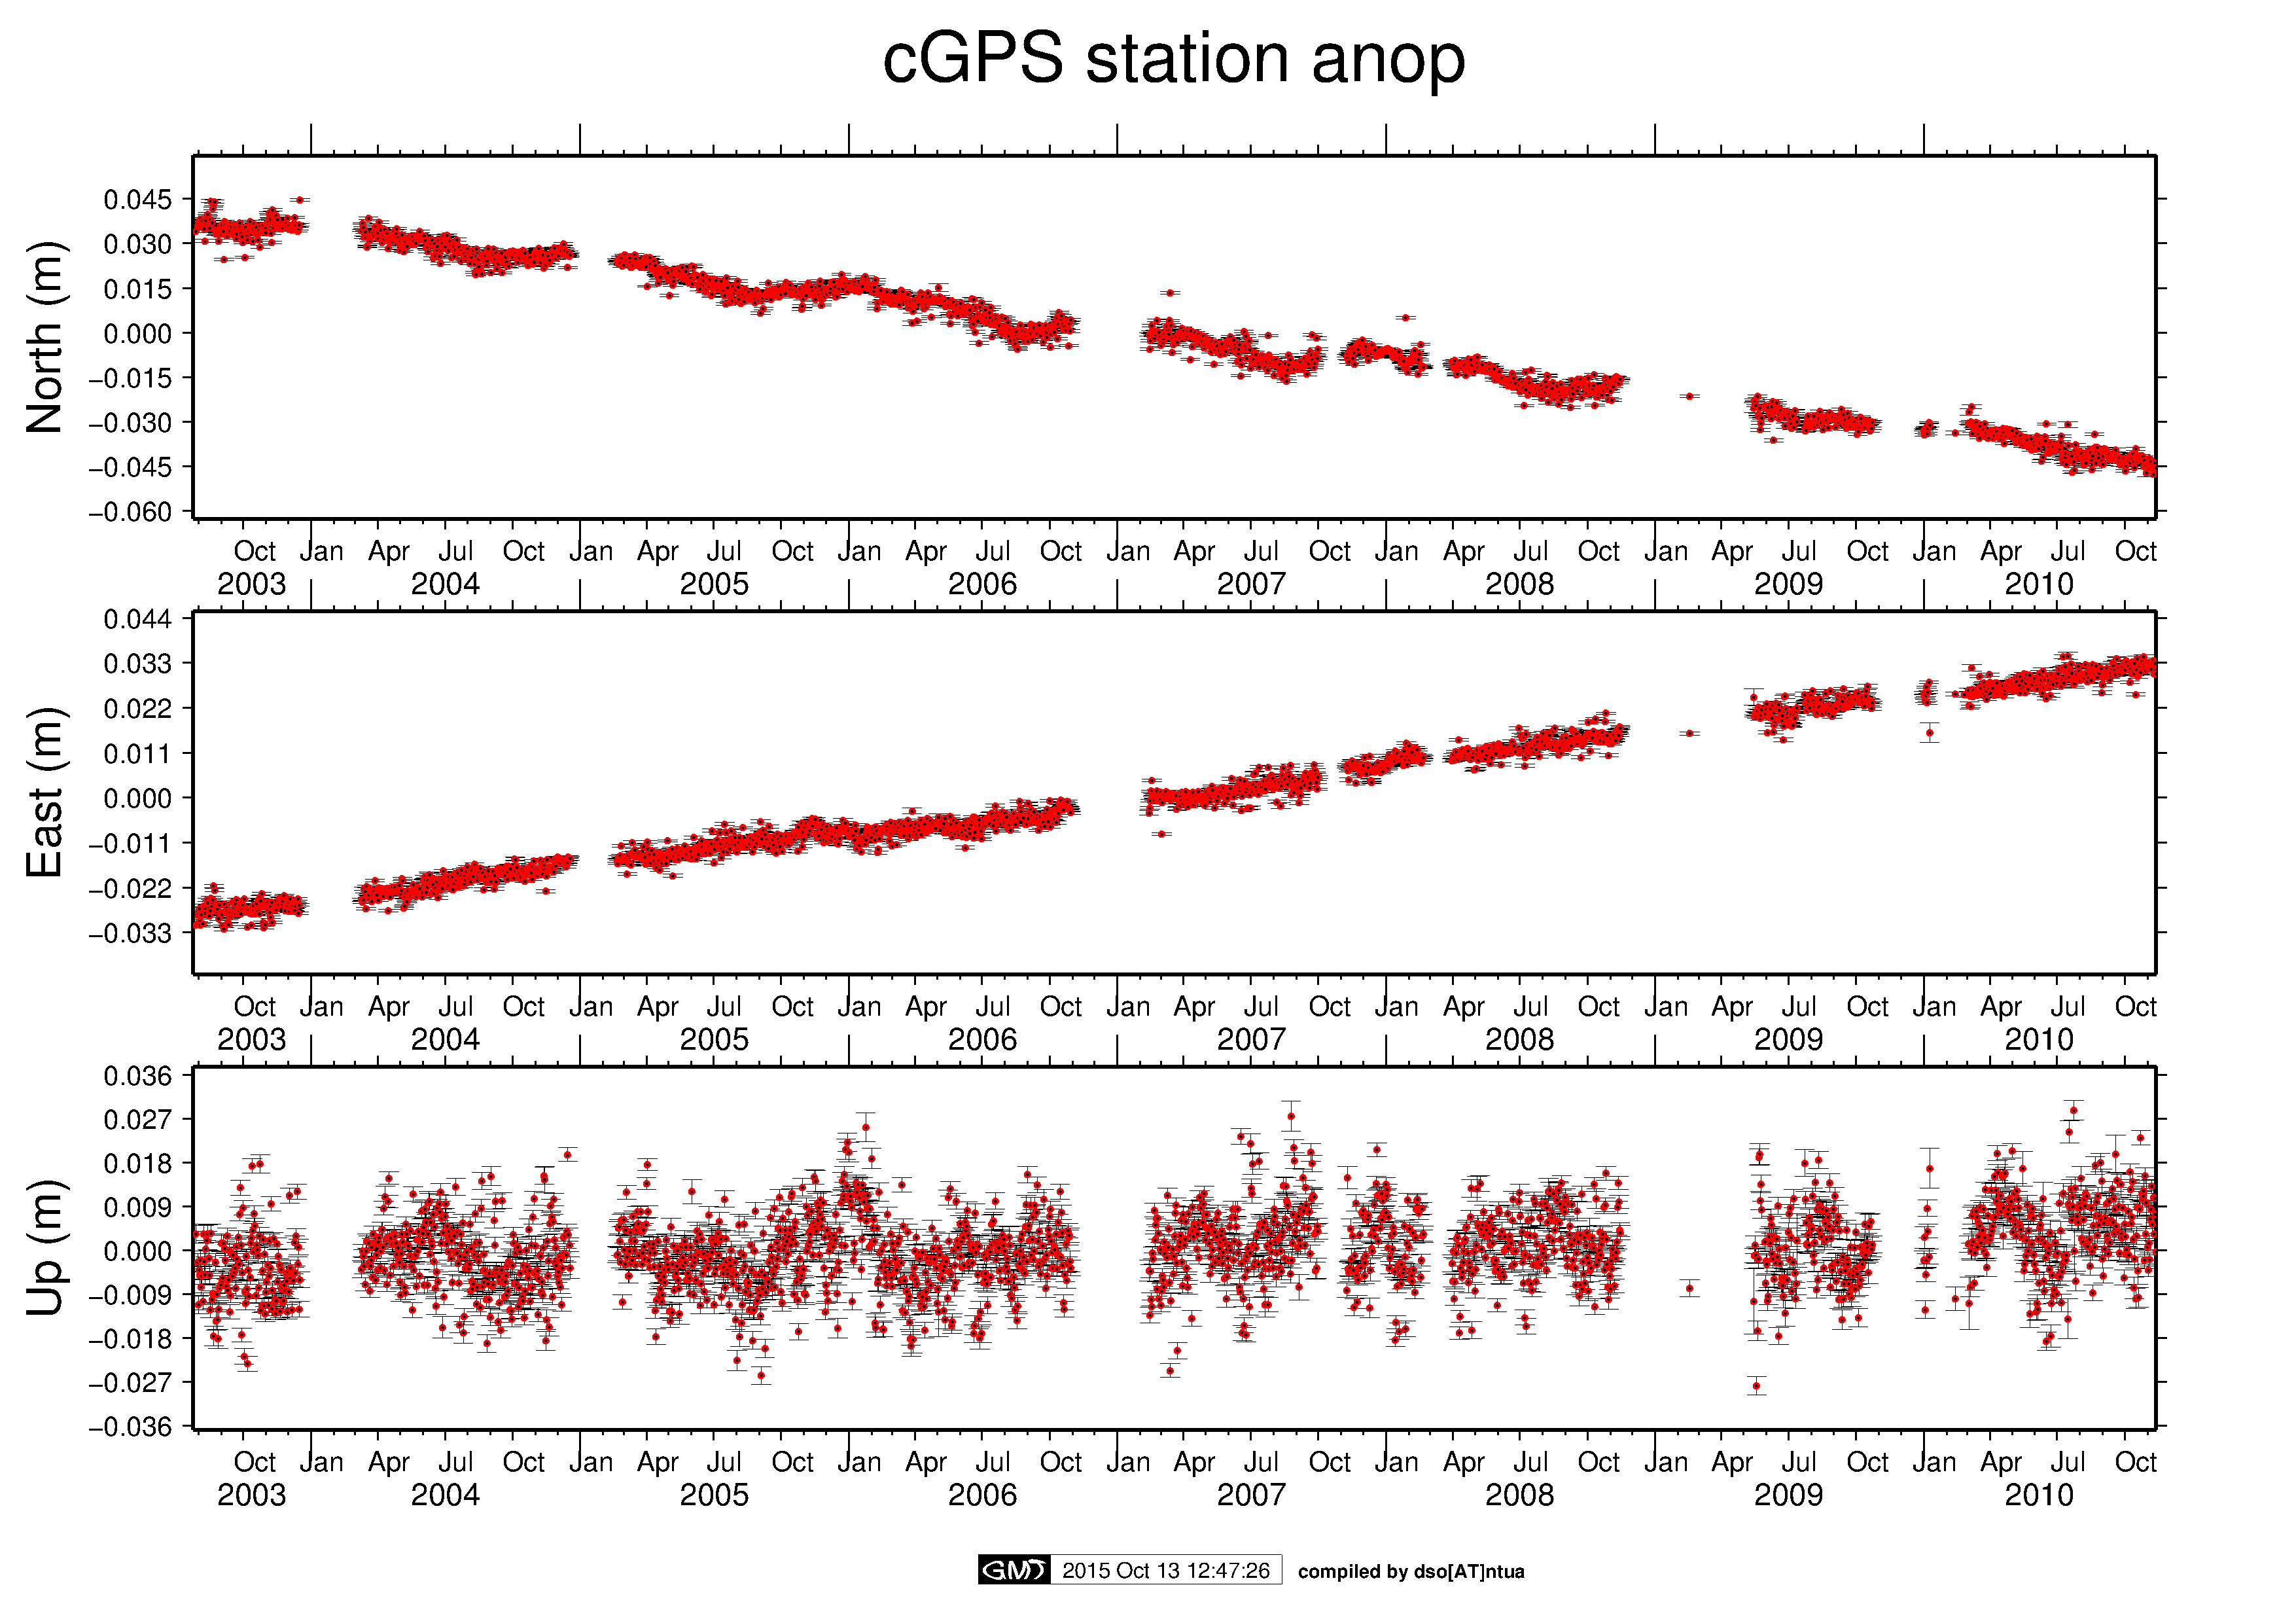
\includegraphics[height=2.6cm]{anop-raw.png}}};
%   \pause
%   \node (img4) at (img2.south west) [yshift=2cm] {\includegraphics[height=4cm]{img/dsoprint.png}};
\end{tikzpicture}
\end{center}
\end{frame}
}

% ------------------------------------------------------------------------------
\begin{frame}
  \frametitle{Cordinate estinmates - Time series analysis}
  \framesubtitle{}
  \label{}

\end{frame}
\note{}

 % ------------------------------------------------------------------------------
\begin{frame}
  \frametitle{Velocity field in Greece}
  \framesubtitle{}
  \label{}
  \vskip-1cm
\begin{columns}[T]
  \begin{column}{.3\textwidth}

  \end{column}
  \begin{column}{.7\textwidth}
    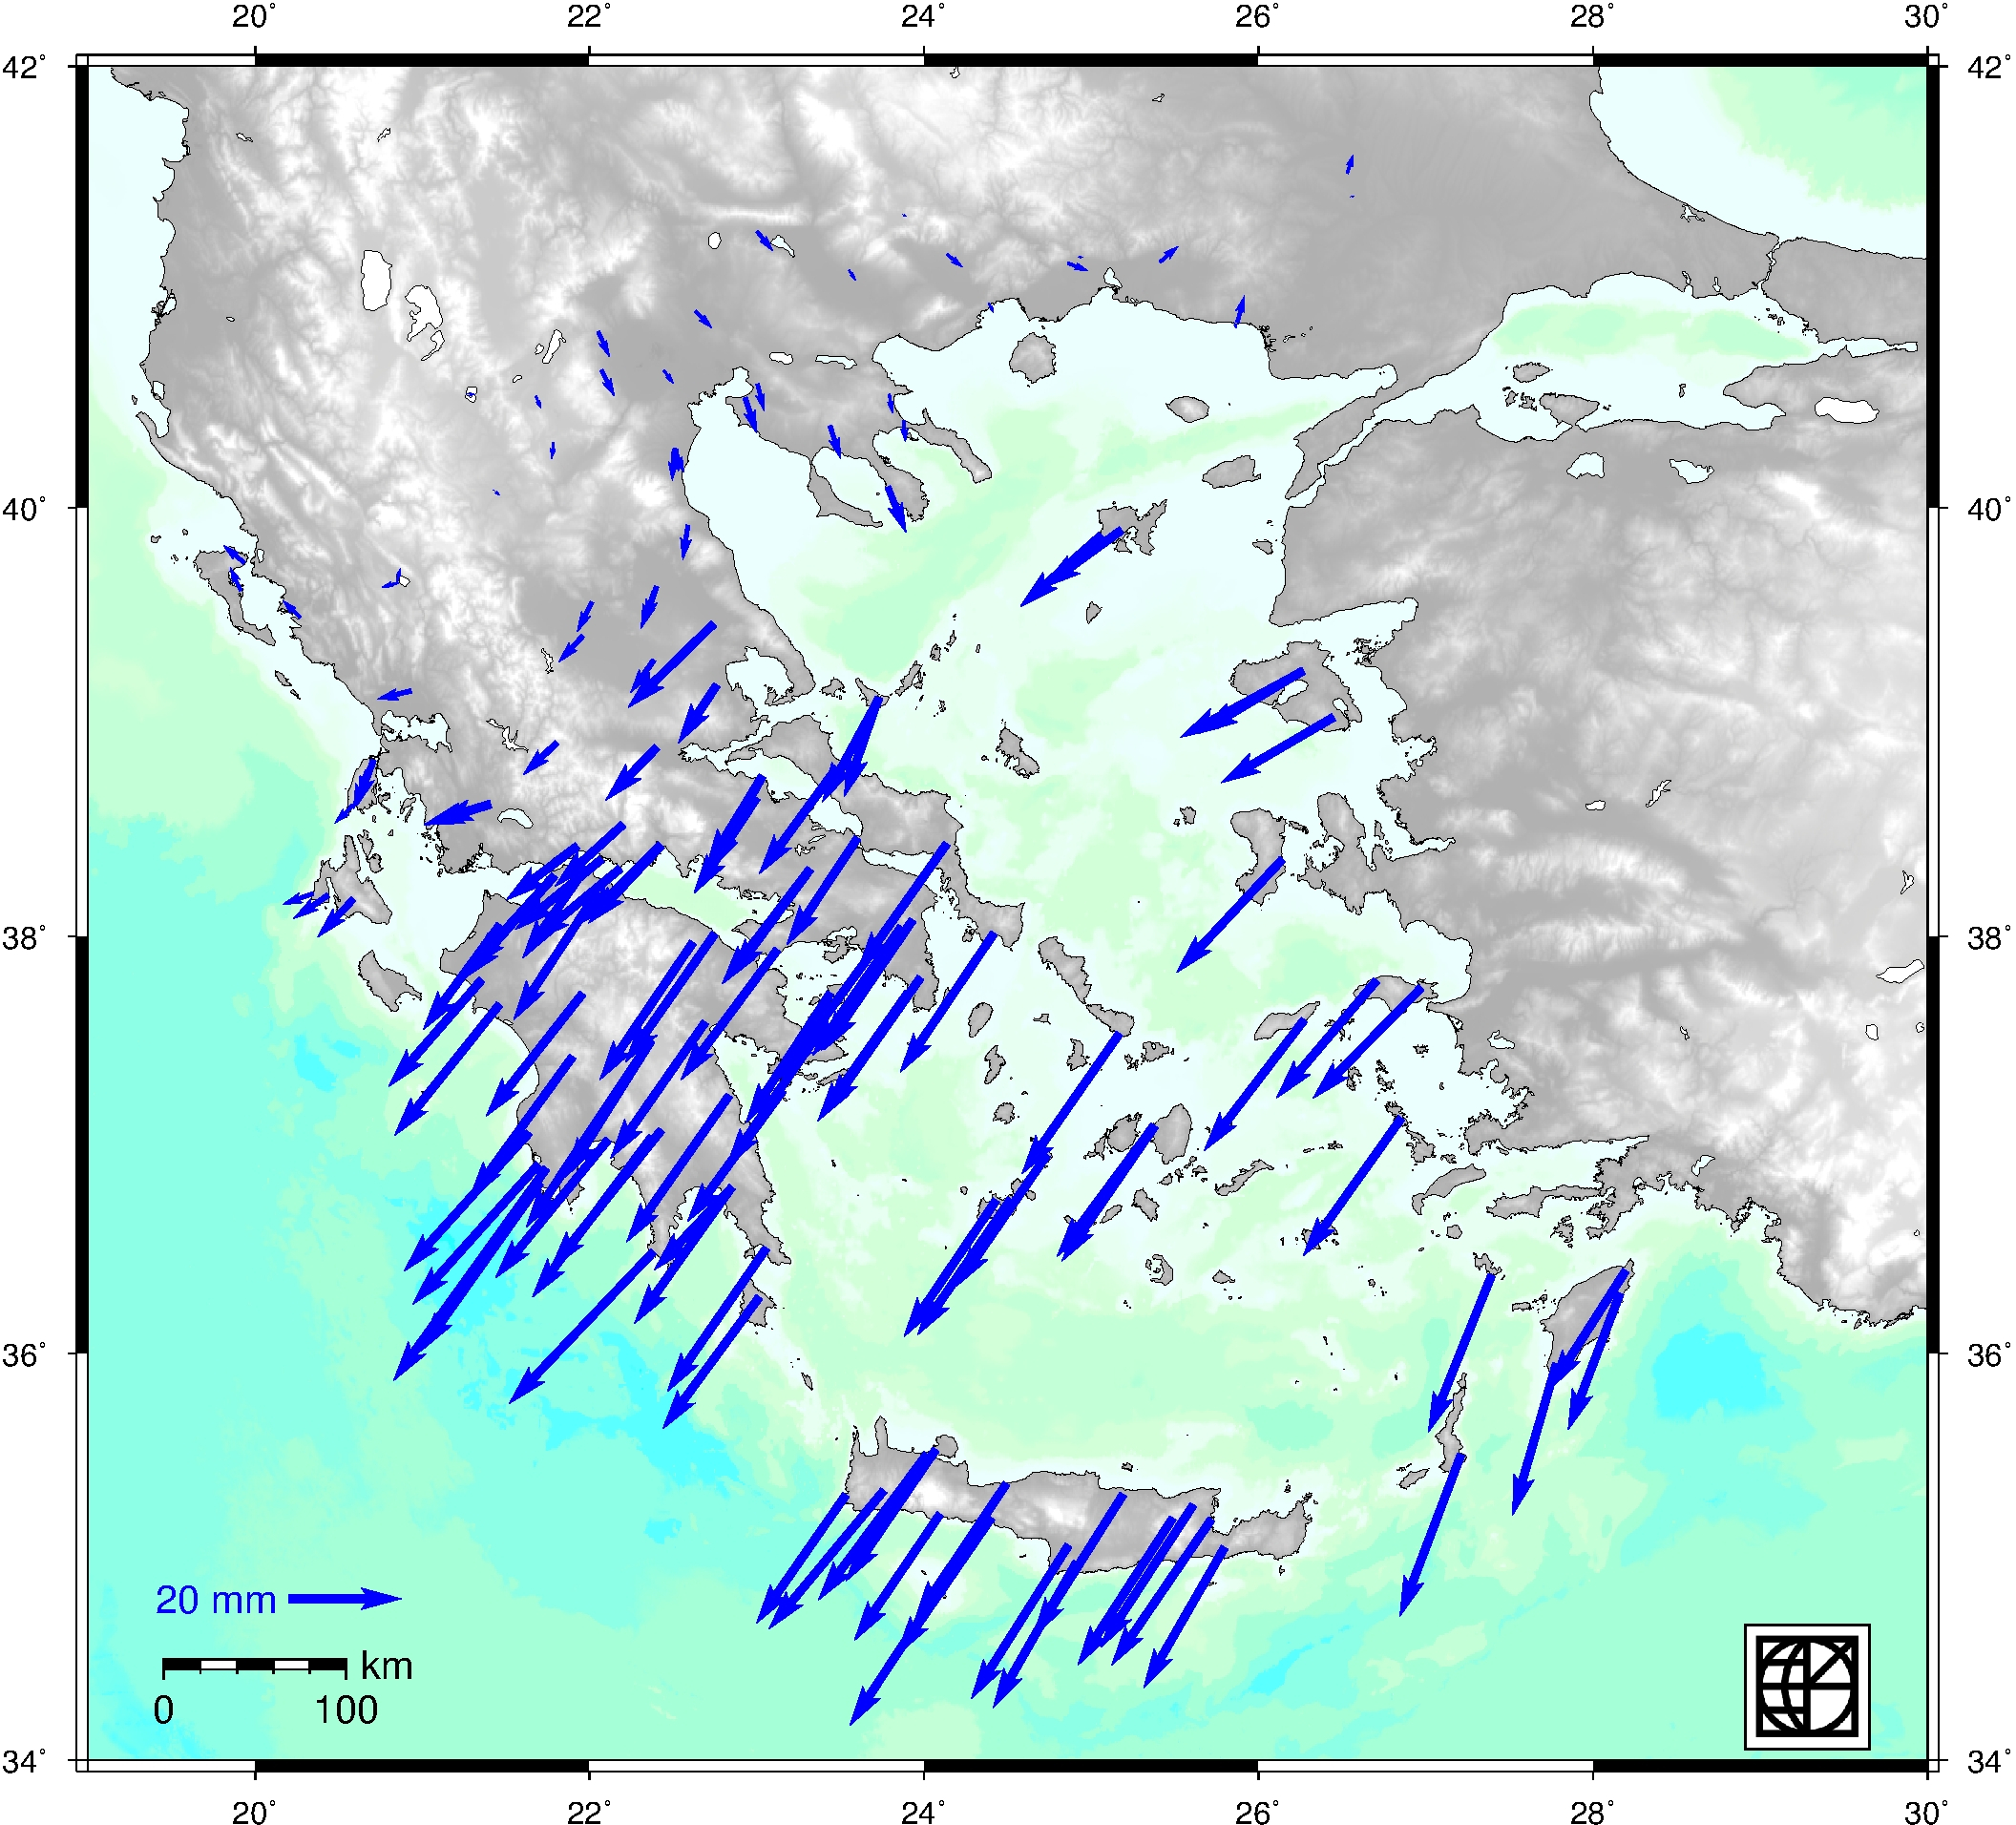
\includegraphics[width=.95\textwidth]{testvel.jpg}
  \end{column}
\end{columns}
\end{frame}
\note{}

 % ------------------------------------------------------------------------------
\begin{frame}
  \frametitle{Focus on specific areas - Corinth Gulf}
  \framesubtitle{}
  \label{}
  
  \begin{center}
    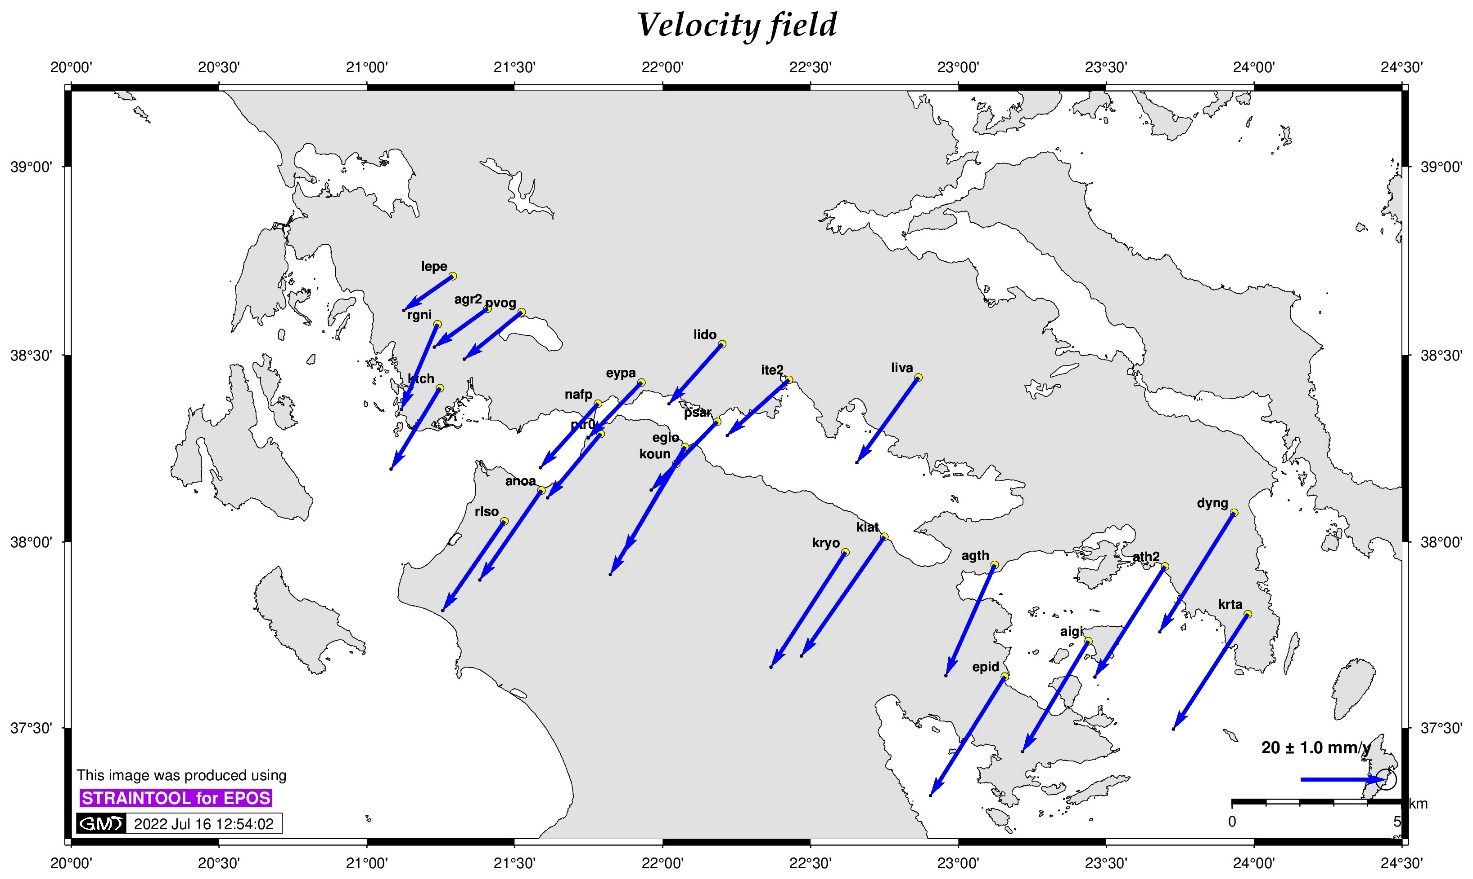
\includegraphics[width=.7\textwidth]{gsg2022_vel.jpg}  
  \end{center}

\end{frame}
\note{}

 % ------------------------------------------------------------------------------
\begin{frame}
  \frametitle{Recent Earthquakes}
  \framesubtitle{}
  \label{}

\end{frame}
\note{}

 % ------------------------------------------------------------------------------
\begin{frame}
  \frametitle{Strain rates}
  \framesubtitle{}
  \label{}
  \vskip-1cm
\begin{columns}[T]
  \begin{column}{.3\textwidth}

  \end{column}
  \begin{column}{.7\textwidth}
      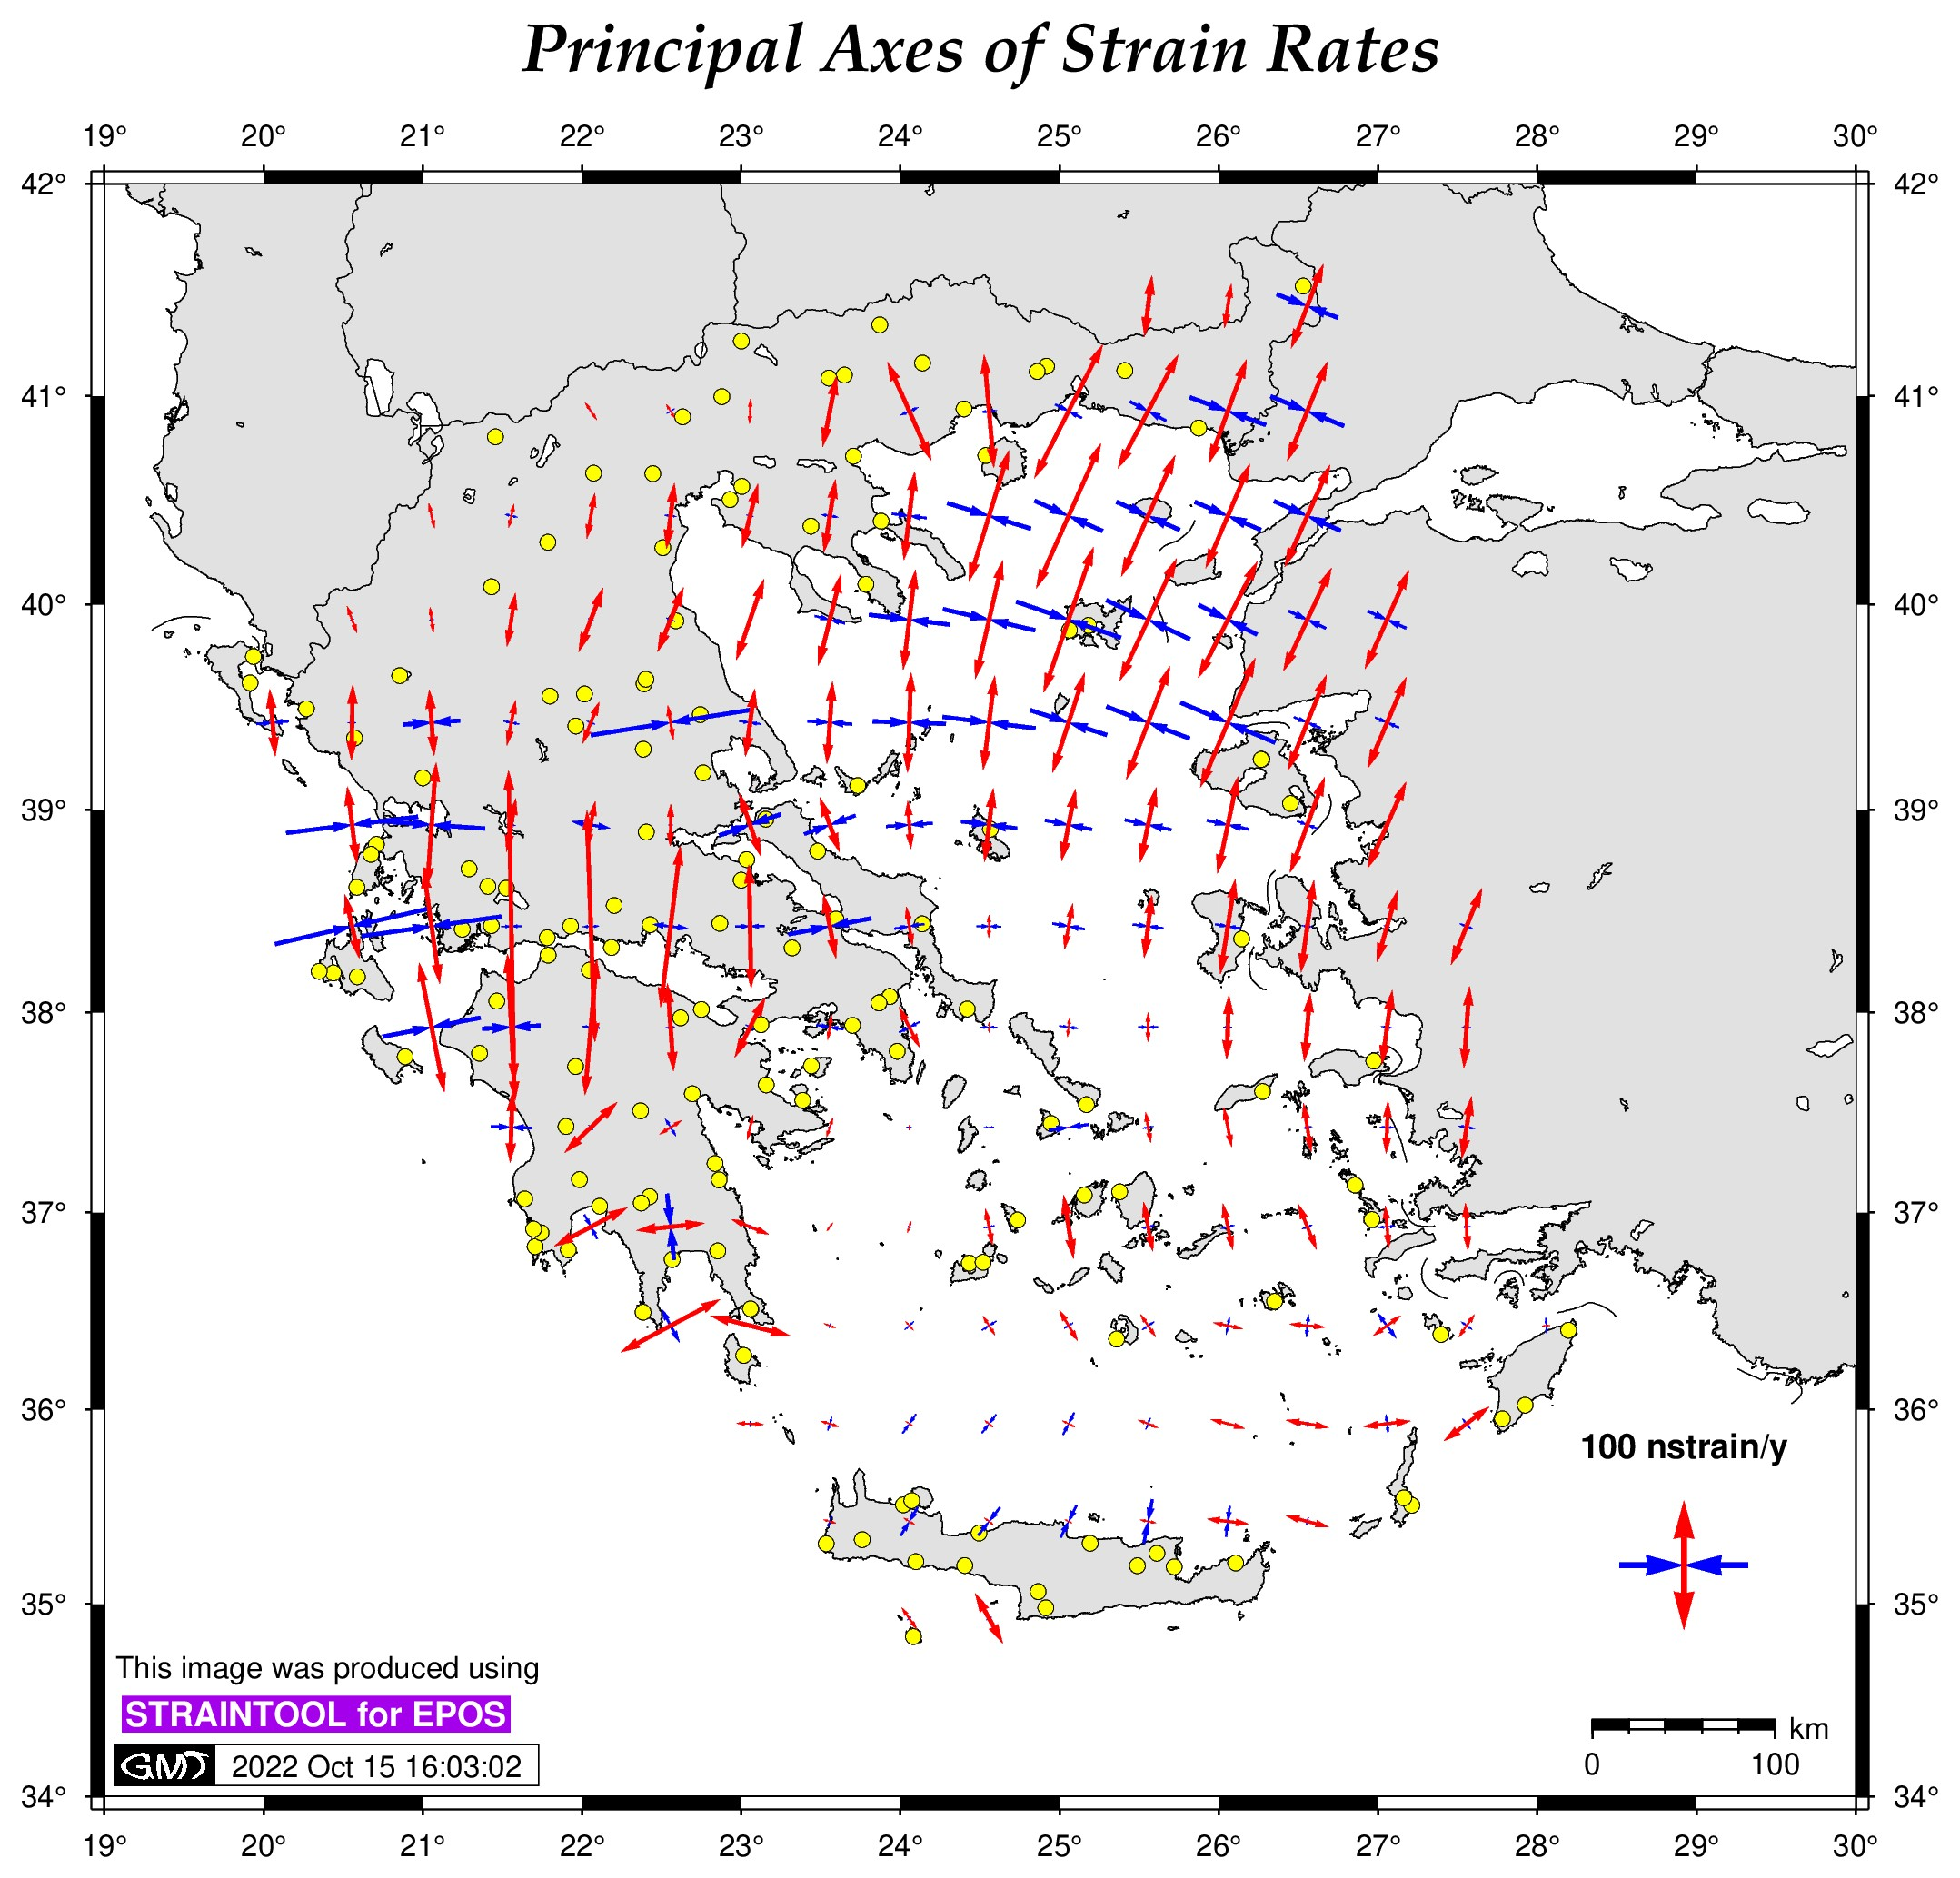
\includegraphics[width=.95\textwidth]{gr-output_str.jpg}
  \end{column}
\end{columns}
\end{frame}
\note{}

 % ------------------------------------------------------------------------------
\begin{frame}
  \frametitle{}
  \framesubtitle{}
  \label{}

\begin{center}
  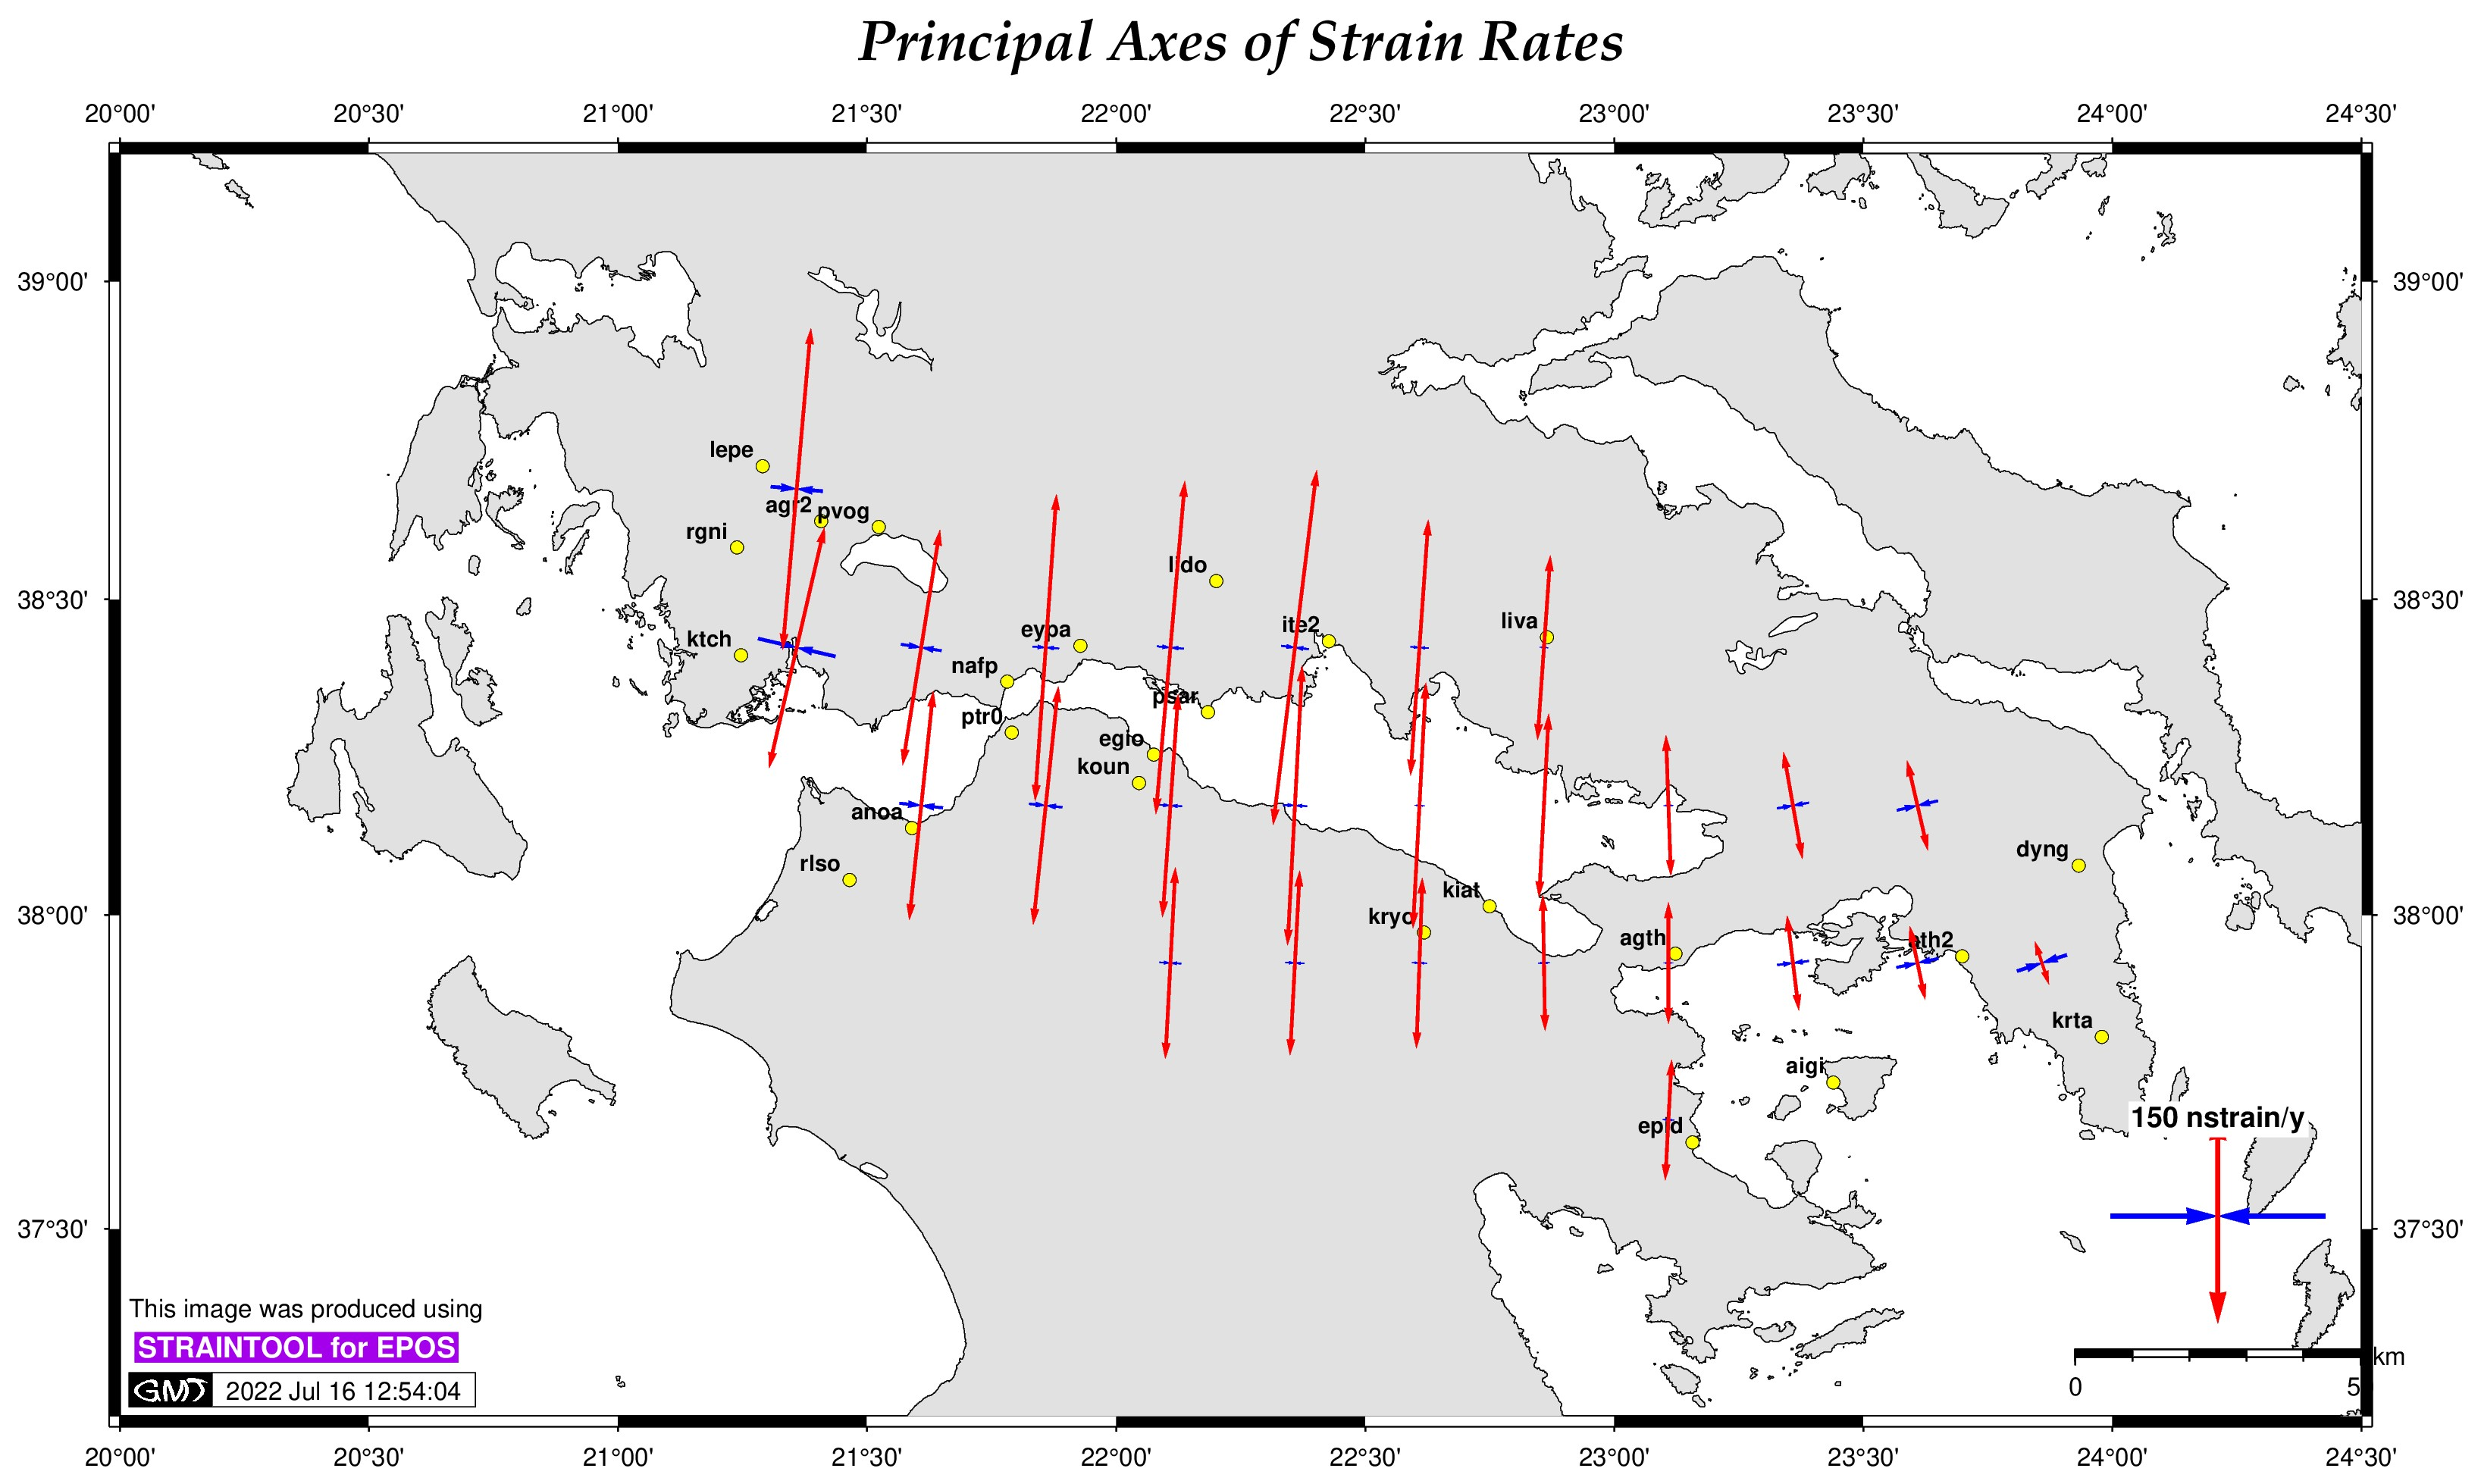
\includegraphics[width=.65\textwidth]{crfeu-output_str.jpg}
\end{center}

\end{frame}
\note{}





\section{Discussion / Conclusions}
 % ------------------------------------------------------------------------------
\begin{frame}
  \frametitle{Discussion / Conclusions}
  \framesubtitle{}
  \label{}

\end{frame}
\note{}


% \section{Open Source Software \textbf{StrainTool v1.0}}
 
% \graphicspath{Figs/}

\begin{frame}
  \frametitle{Open Source Software \textbf{StrainTool v1.0}}
  \framesubtitle{}
  \label{ch2:straintool}
  
  StrainTool has three basic components:
  \begin{itemize}
    \item \textbf{pystrain:} A python pachage.
    \item \textbf{StrainTensor.py:} the main executable.
    \item A list of shell scripts to plot results from StrainTensor.py
  \end{itemize}
  \textcolor{red}{TODO: structure design}
  
\end{frame}
\note{}


\begin{frame}
  \frametitle{Python Package \texttt{pystrain}}
  \framesubtitle{}
  \label{ch2:}
  
  \texttt{pystrain} the core part of the project.
  
  Python functions and classes, enable computation of strain tensor.
  
  The package includes:
  \begin{itemize}
    \item \texttt{iotools}: input/output classes to parse ASCII files.
    \item \texttt{geodesy}: functions for basic geodetic calculations.
    \item \texttt{grid.py}: a simple grid generator
    \item \texttt{strain.py}: main class and necessary functions for estimation of strain  tensor parameters
  \end{itemize}
  
  

\end{frame}
\note{}


\begin{frame}
 \frametitle{Estimate strain tensor parameters}
 \framesubtitle{}
 \label{ch2:}

\end{frame}
\note{}

\begin{frame}
 \frametitle{Shen Algorithm}
 \framesubtitle{}
 \label{ch2:}

\end{frame}
\note{}


\begin{frame}
 \frametitle{Shen Algorithm}
 \framesubtitle{Distance-dependent weighting}
 \label{ch2:}

\end{frame}
\note{}

\begin{frame}
 \frametitle{Shen Algorithm}
 \framesubtitle{Optimal smoothin parameter D}
 \label{ch2:}

\end{frame}
\note{}

\begin{frame}
 \frametitle{Shen Algorithm}
 \framesubtitle{Spatial weights}
 \label{ch2:}

\end{frame}
\note{}

\begin{frame}
 \frametitle{Veis Algorithm}
 \framesubtitle{}
 \label{ch2:}

\end{frame}
\note{}



%\begin{frame}
%   \frametitle{}
%   \framesubtitle{}
%   \label{ch2:}

%\end{frame}
%\note{}

% \section{Data analysis and Validation}

\graphicspath{{Chapter3/Figs/}}

\begin{frame}
  \frametitle{Input Datasets}
  \framesubtitle{}
  \label{ch3:data}
  
  \textbf{For validation:}
  \begin{enumerate}
    \item EPN network, solution C2010 - ETRF 2014 (299 stations)
    \item EPOS network, INGV solution (571 stations)
    \item EPOS network, CNRS solution (MIDAS) (452 stations)
    \item network GREECE, NTUA reprocessing 2017 (153 stations)
  \end{enumerate}
    
\end{frame}
\note{}

\begin{frame}
  \frametitle{Validation}
  \framesubtitle{emax - emin maps comparison}
  \label{ch3:data}
  \textcolor{red}{TODO: datasets}
  \begin{columns}
    \begin{column}{0.5\textwidth}
      VISR
      
      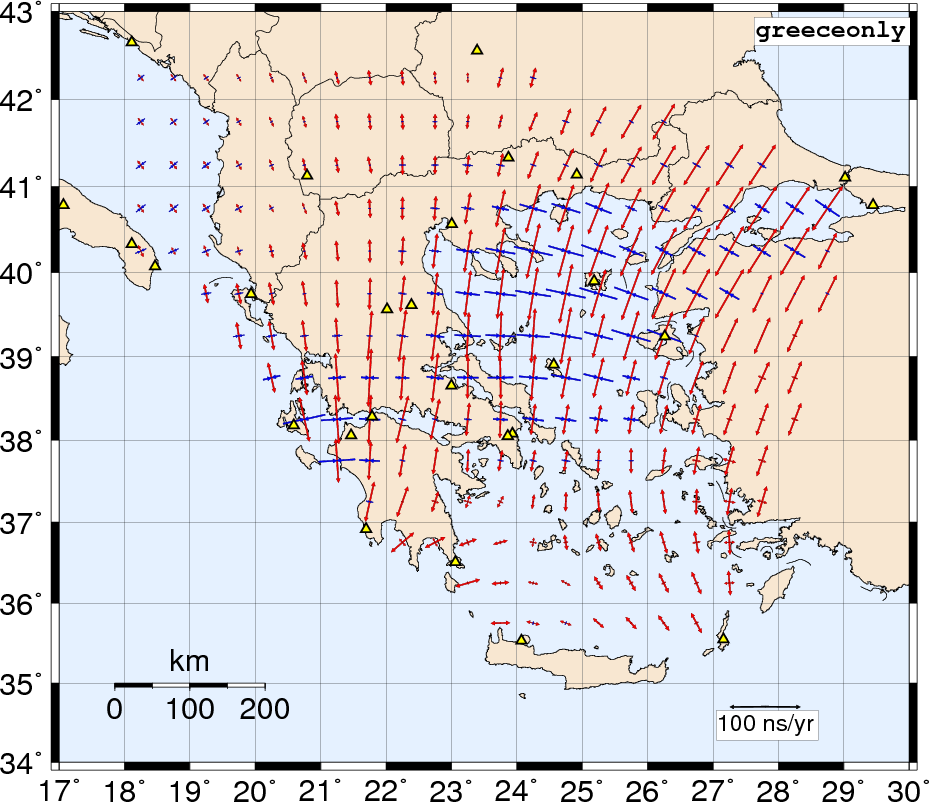
\includegraphics[width=.9\textwidth]{a1_map_strain_vectors.png}   
    \end{column}
    \begin{column}{0.5\textwidth}
    \begin{center}
      PyStrain
      
      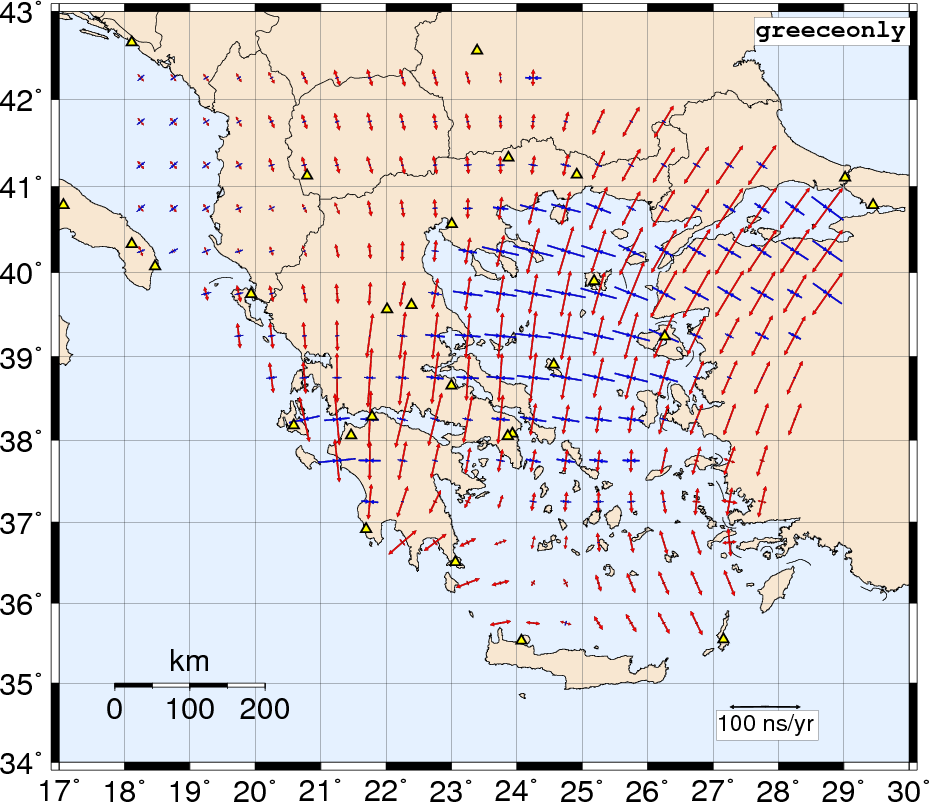
\includegraphics[width=0.9\textwidth]{a2_map_strain_vectors.png}     
    \end{center}
    \end{column}
  \end{columns}

\end{frame}
\note{}

% \begin{frame}
%   \frametitle{Validation}
%   \framesubtitle{dilatation maps comparison}
%   \label{ch3:data}
%   \textcolor{red}{maybe a wrong dataset}
%   \begin{columns}
%     \begin{column}{0.5\textwidth}
%       VISR
%       
%       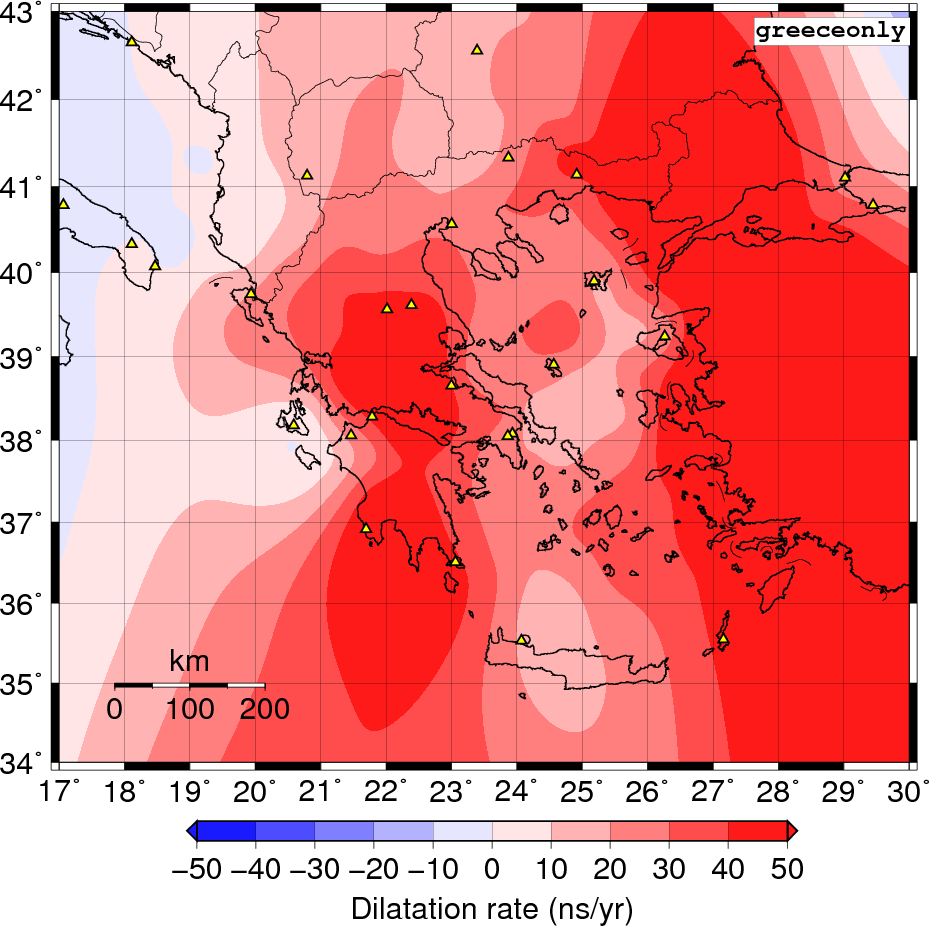
\includegraphics[width=.9\textwidth]{b1_map_strain_dilatation.png}   
%     \end{column}
%     \begin{column}{0.5\textwidth}
%     \begin{center}
%       PyStrain
%       
%       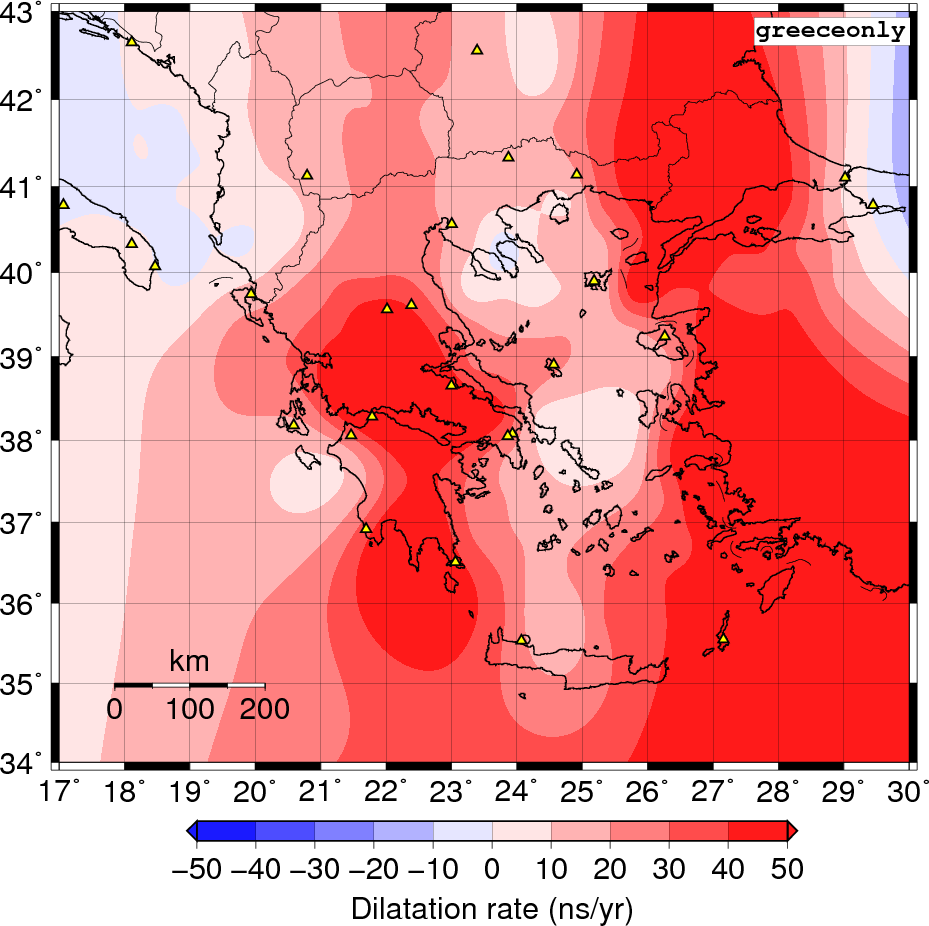
\includegraphics[width=0.9\textwidth]{b2_map_strain_dilatation.png}     
%     \end{center}
%     \end{column}
%   \end{columns}
% 
% \end{frame}
% \note{}

\begin{frame}
  \frametitle{Validation}
  \framesubtitle{differences}
  \label{ch3:data}
  
  \begin{columns}
    \begin{column}{0.5\textwidth}
     
      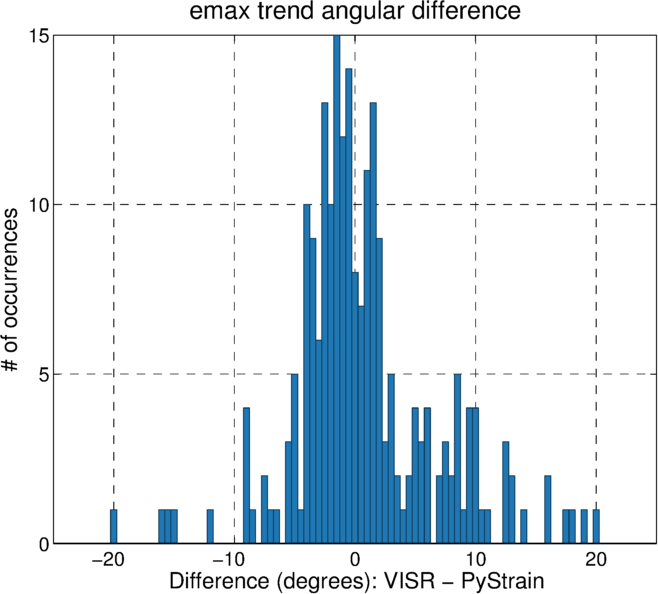
\includegraphics[width=.7\textwidth]{diff-emax-trend_VISR-vs-PyStrain.png}
      
      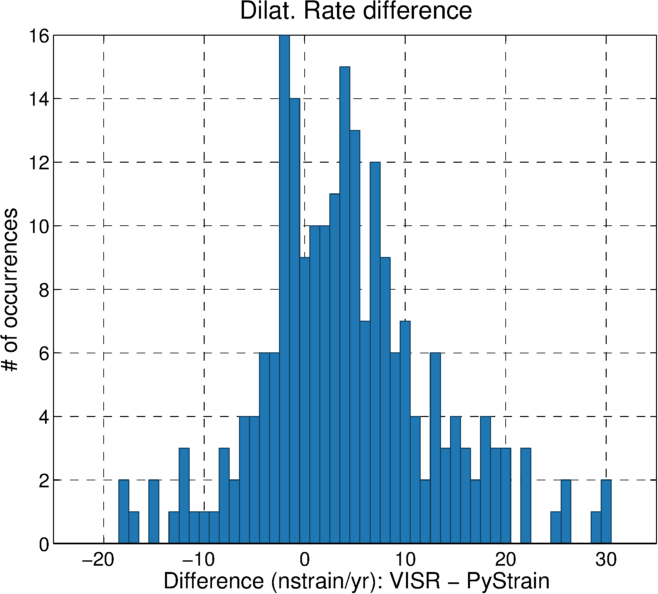
\includegraphics[width=.7\textwidth]{diff-dilat_VISR-vs-PyStrain.png}
    \end{column}
    \begin{column}{0.5\textwidth}
    \begin{center}
      
      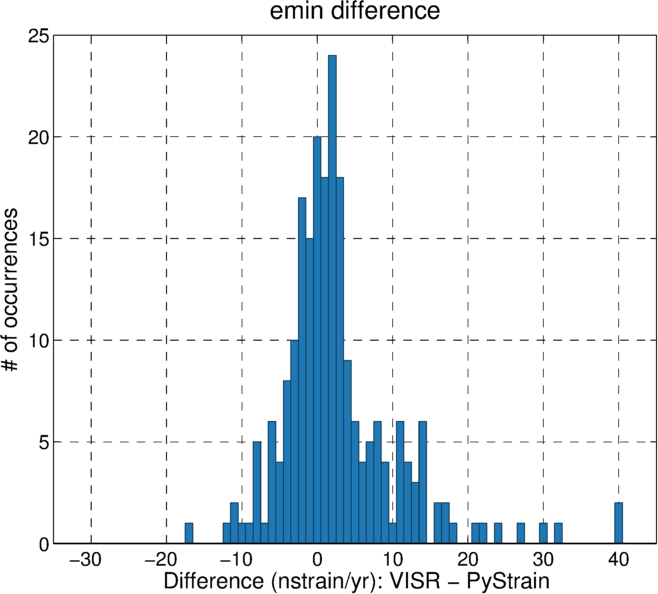
\includegraphics[width=.7\textwidth]{diff-emin_VISR-vs-PyStrain.png}
      
      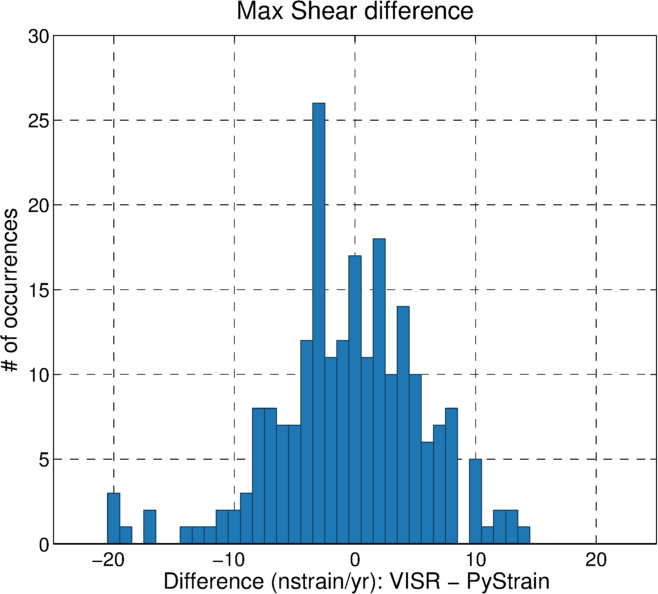
\includegraphics[width=.7\textwidth]{diff-shear_VISR-vs-PyStrain.png}     
    \end{center}
    \end{column}
  \end{columns}

\end{frame}
\note{}

\begin{frame}
  \frametitle{Validation}
  \framesubtitle{histograms}
  \label{ch3:data}
  
  \begin{columns}
    \begin{column}{0.5\textwidth}
     
      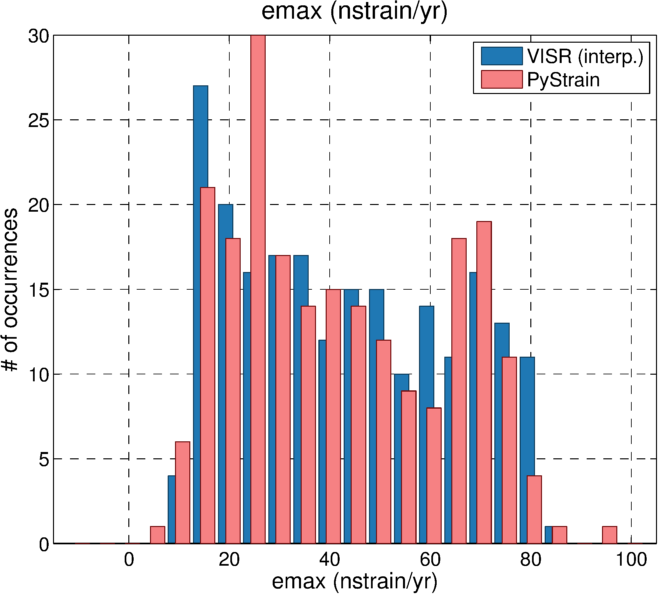
\includegraphics[width=.7\textwidth]{emax_hist_VISR-vs-PyStrain.png}
      
      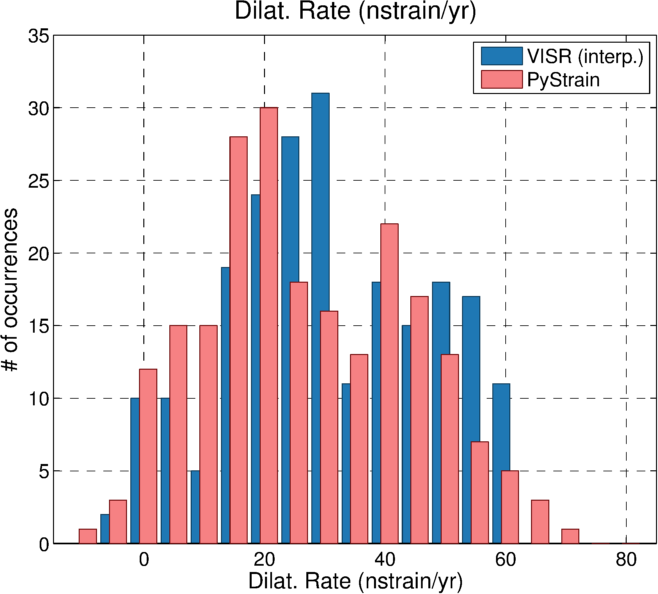
\includegraphics[width=.7\textwidth]{dilat_hist_VISR-vs-PyStrain.png}
    \end{column}
    \begin{column}{0.5\textwidth}
    \begin{center}
      
      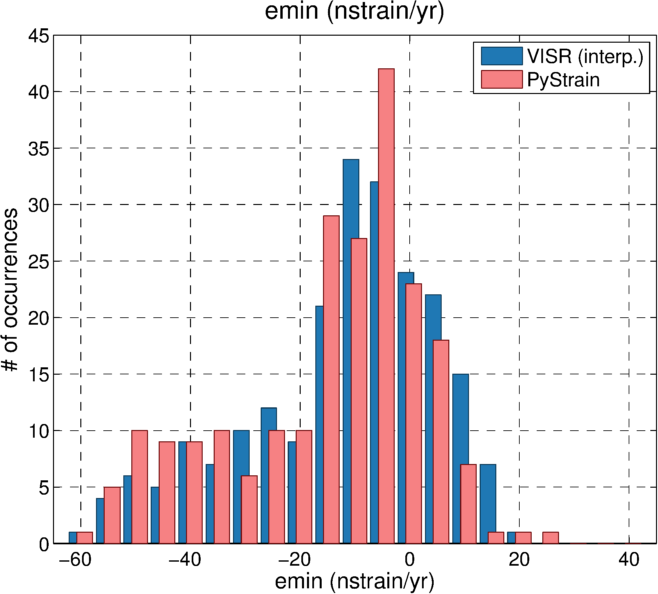
\includegraphics[width=.7\textwidth]{emin_hist_VISR-vs-PyStrain.png}
      
      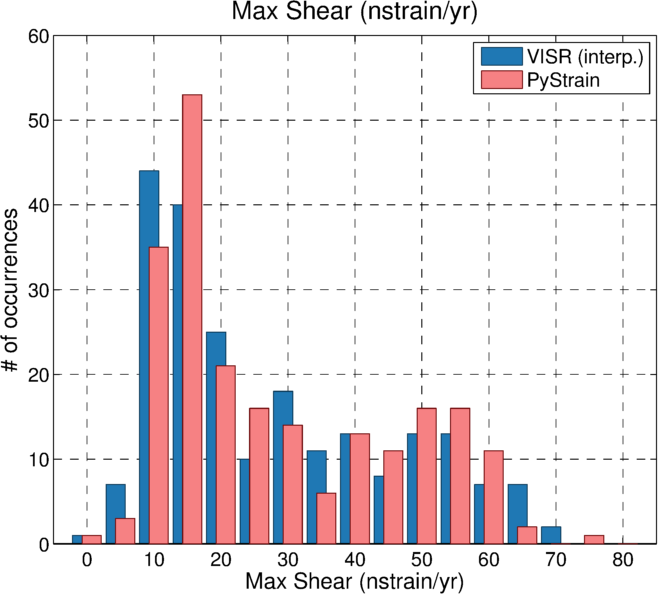
\includegraphics[width=.7\textwidth]{shear_hist_VISR-vs-PyStrain.png}     
    \end{center}
    \end{column}
  \end{columns}

\end{frame}
\note{}


%\begin{frame}
%  \frametitle{Συμπεράσματα}
%  \framesubtitle{}
%  \label{ch3:}

%\end{frame}
%\note{}

% \section{Strain Analysis and Discussion}
 
\graphicspath{{Chapter4/Figs/}}

\begin{frame}
 \frametitle{Strain Analysis}
 \framesubtitle{}
 \label{ch4:}
 
  Model parameters fr Shen algorithm
  
  Data Set: MIDAS
  \begin{itemize}
    \item Wt=6
    \item dmin = 1km
    \item dmax = 500km
    \item dstep = 1km
    \item ltype = gaussian
    \item x step = y step = 0.5 $^{\circ}$
    \item region = Greece: 18/30/34/43 -  Italy: 4/18/32/48
  \end{itemize}

\end{frame}
\note{}

\begin{frame}
 \frametitle{Strain Analysis}
 \framesubtitle{Greece region}
 \label{ch4:}
   
  \begin{columns}
    \begin{column}{0.5\textwidth}
      
      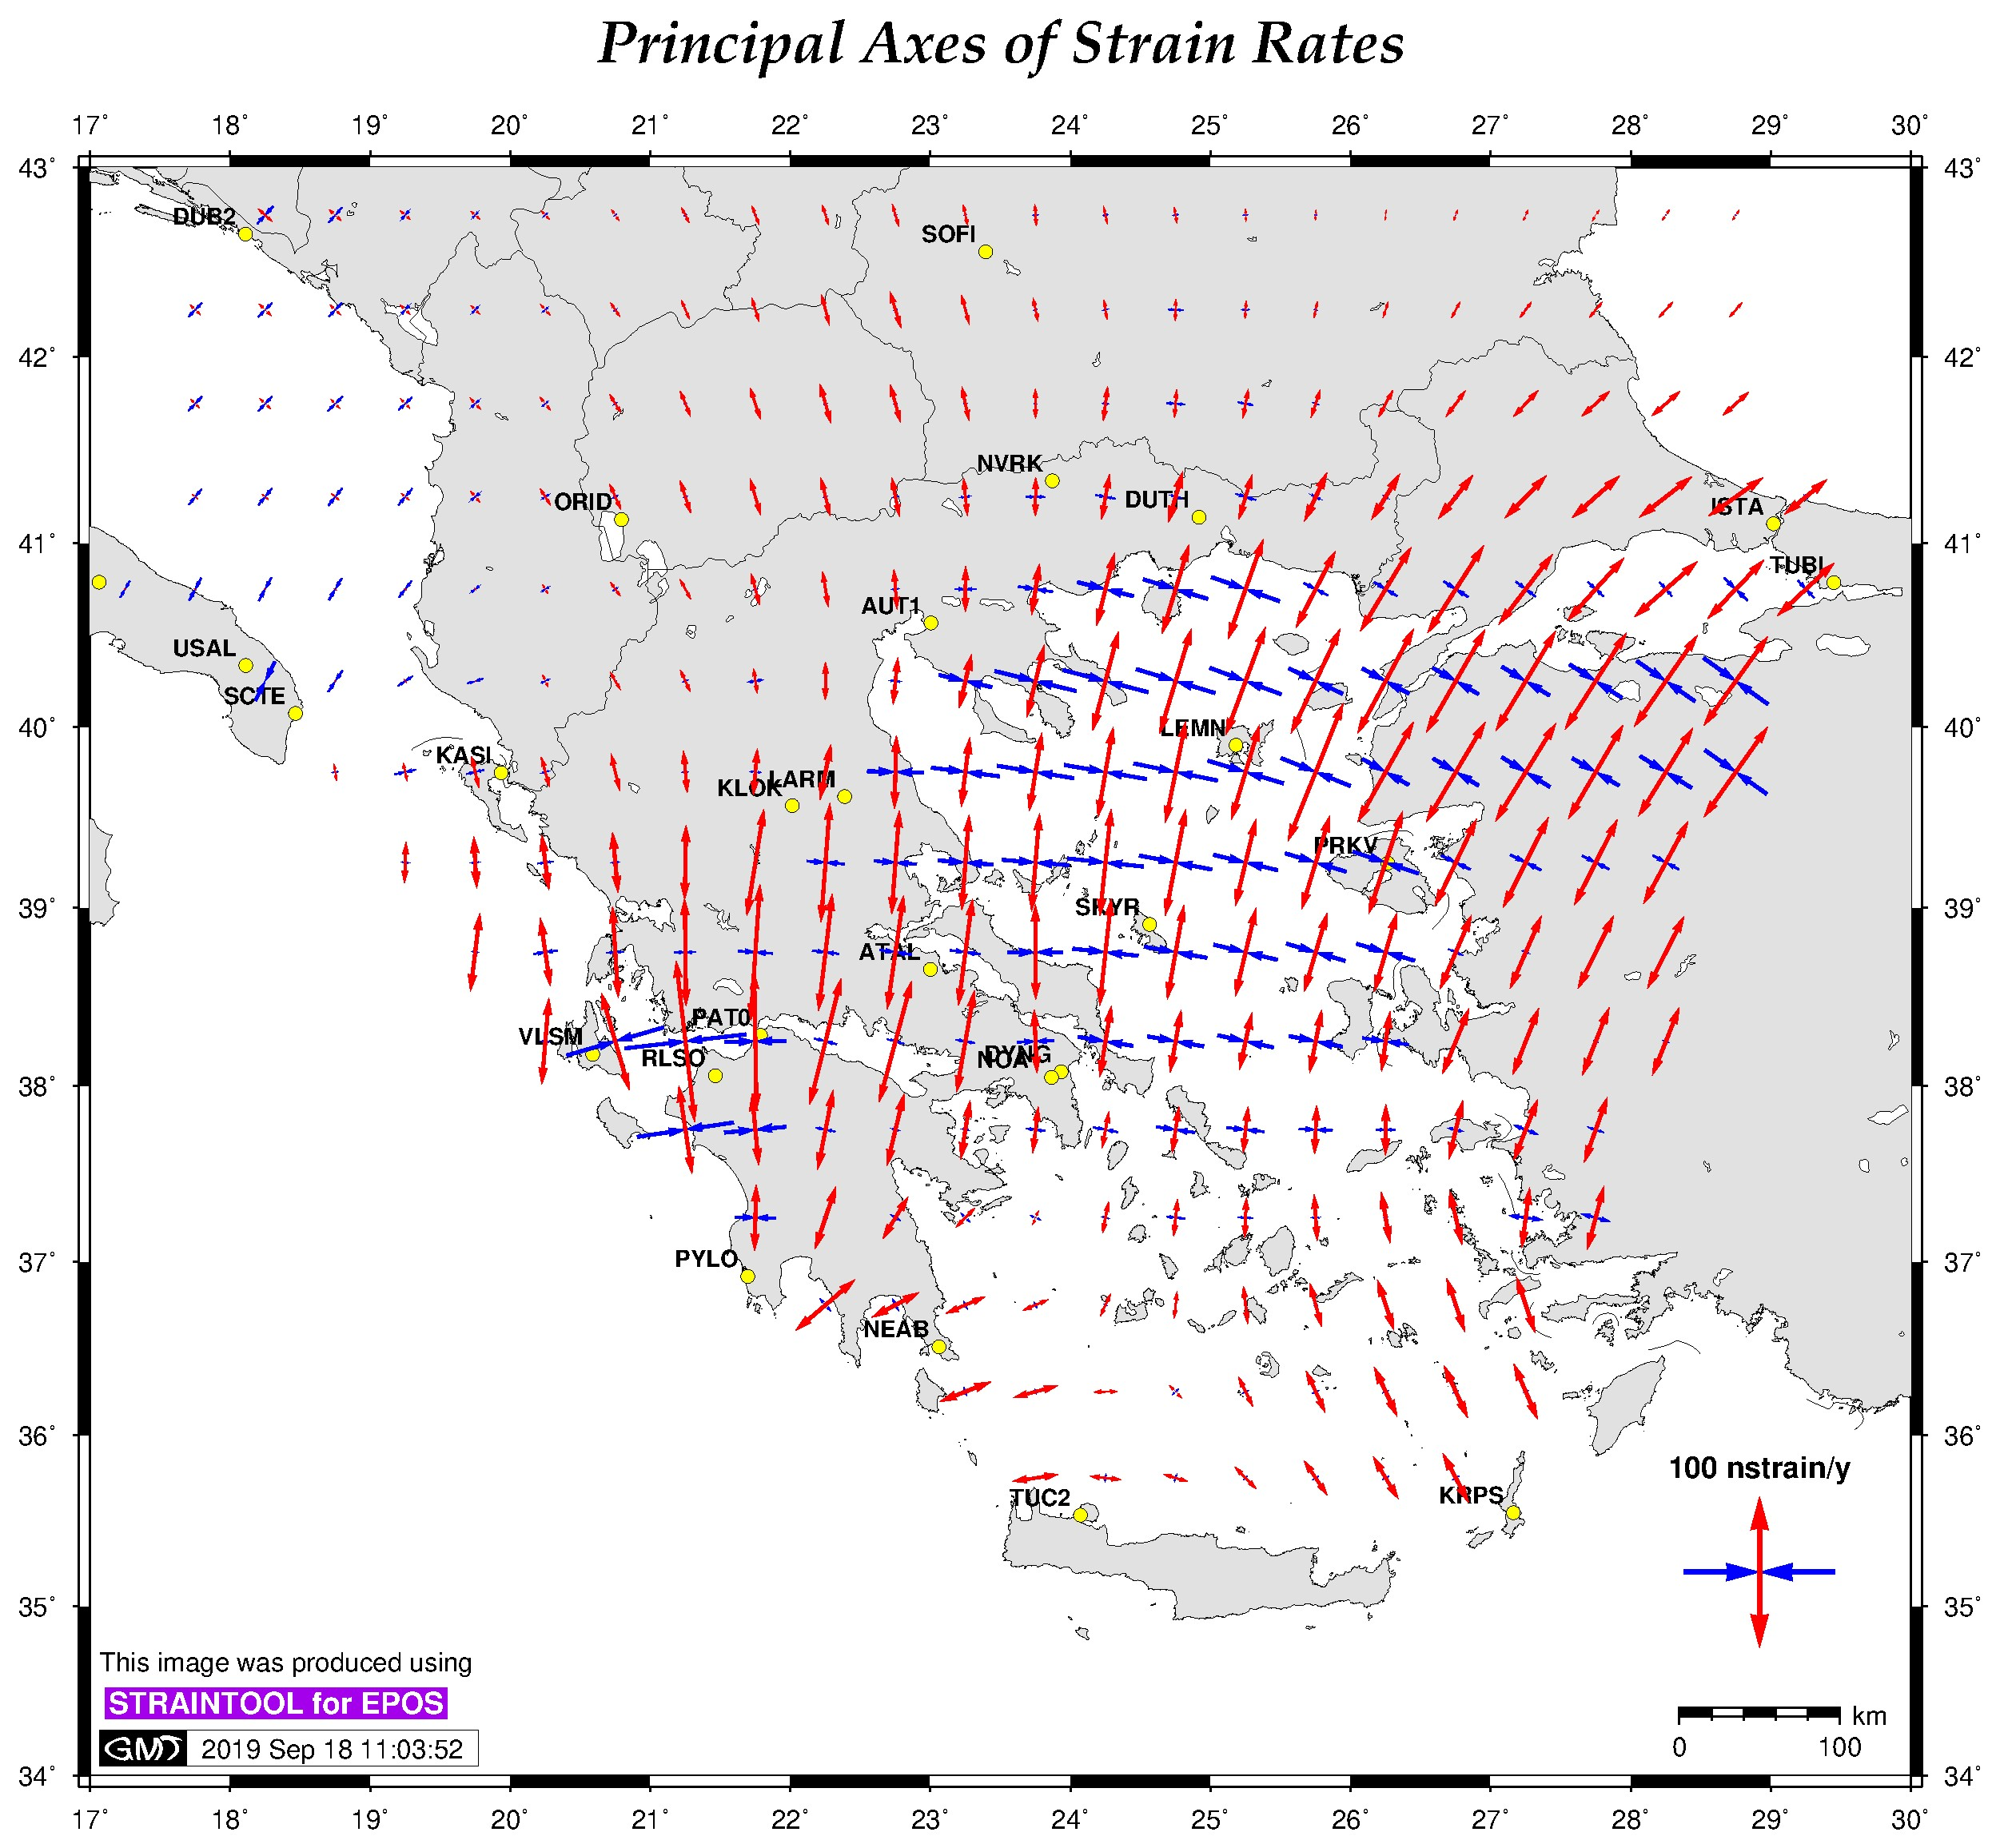
\includegraphics[width=.9\textwidth]{grmidas-output_str.jpg}   
    \end{column}
    \begin{column}{0.5\textwidth}
    \begin{center}
      
      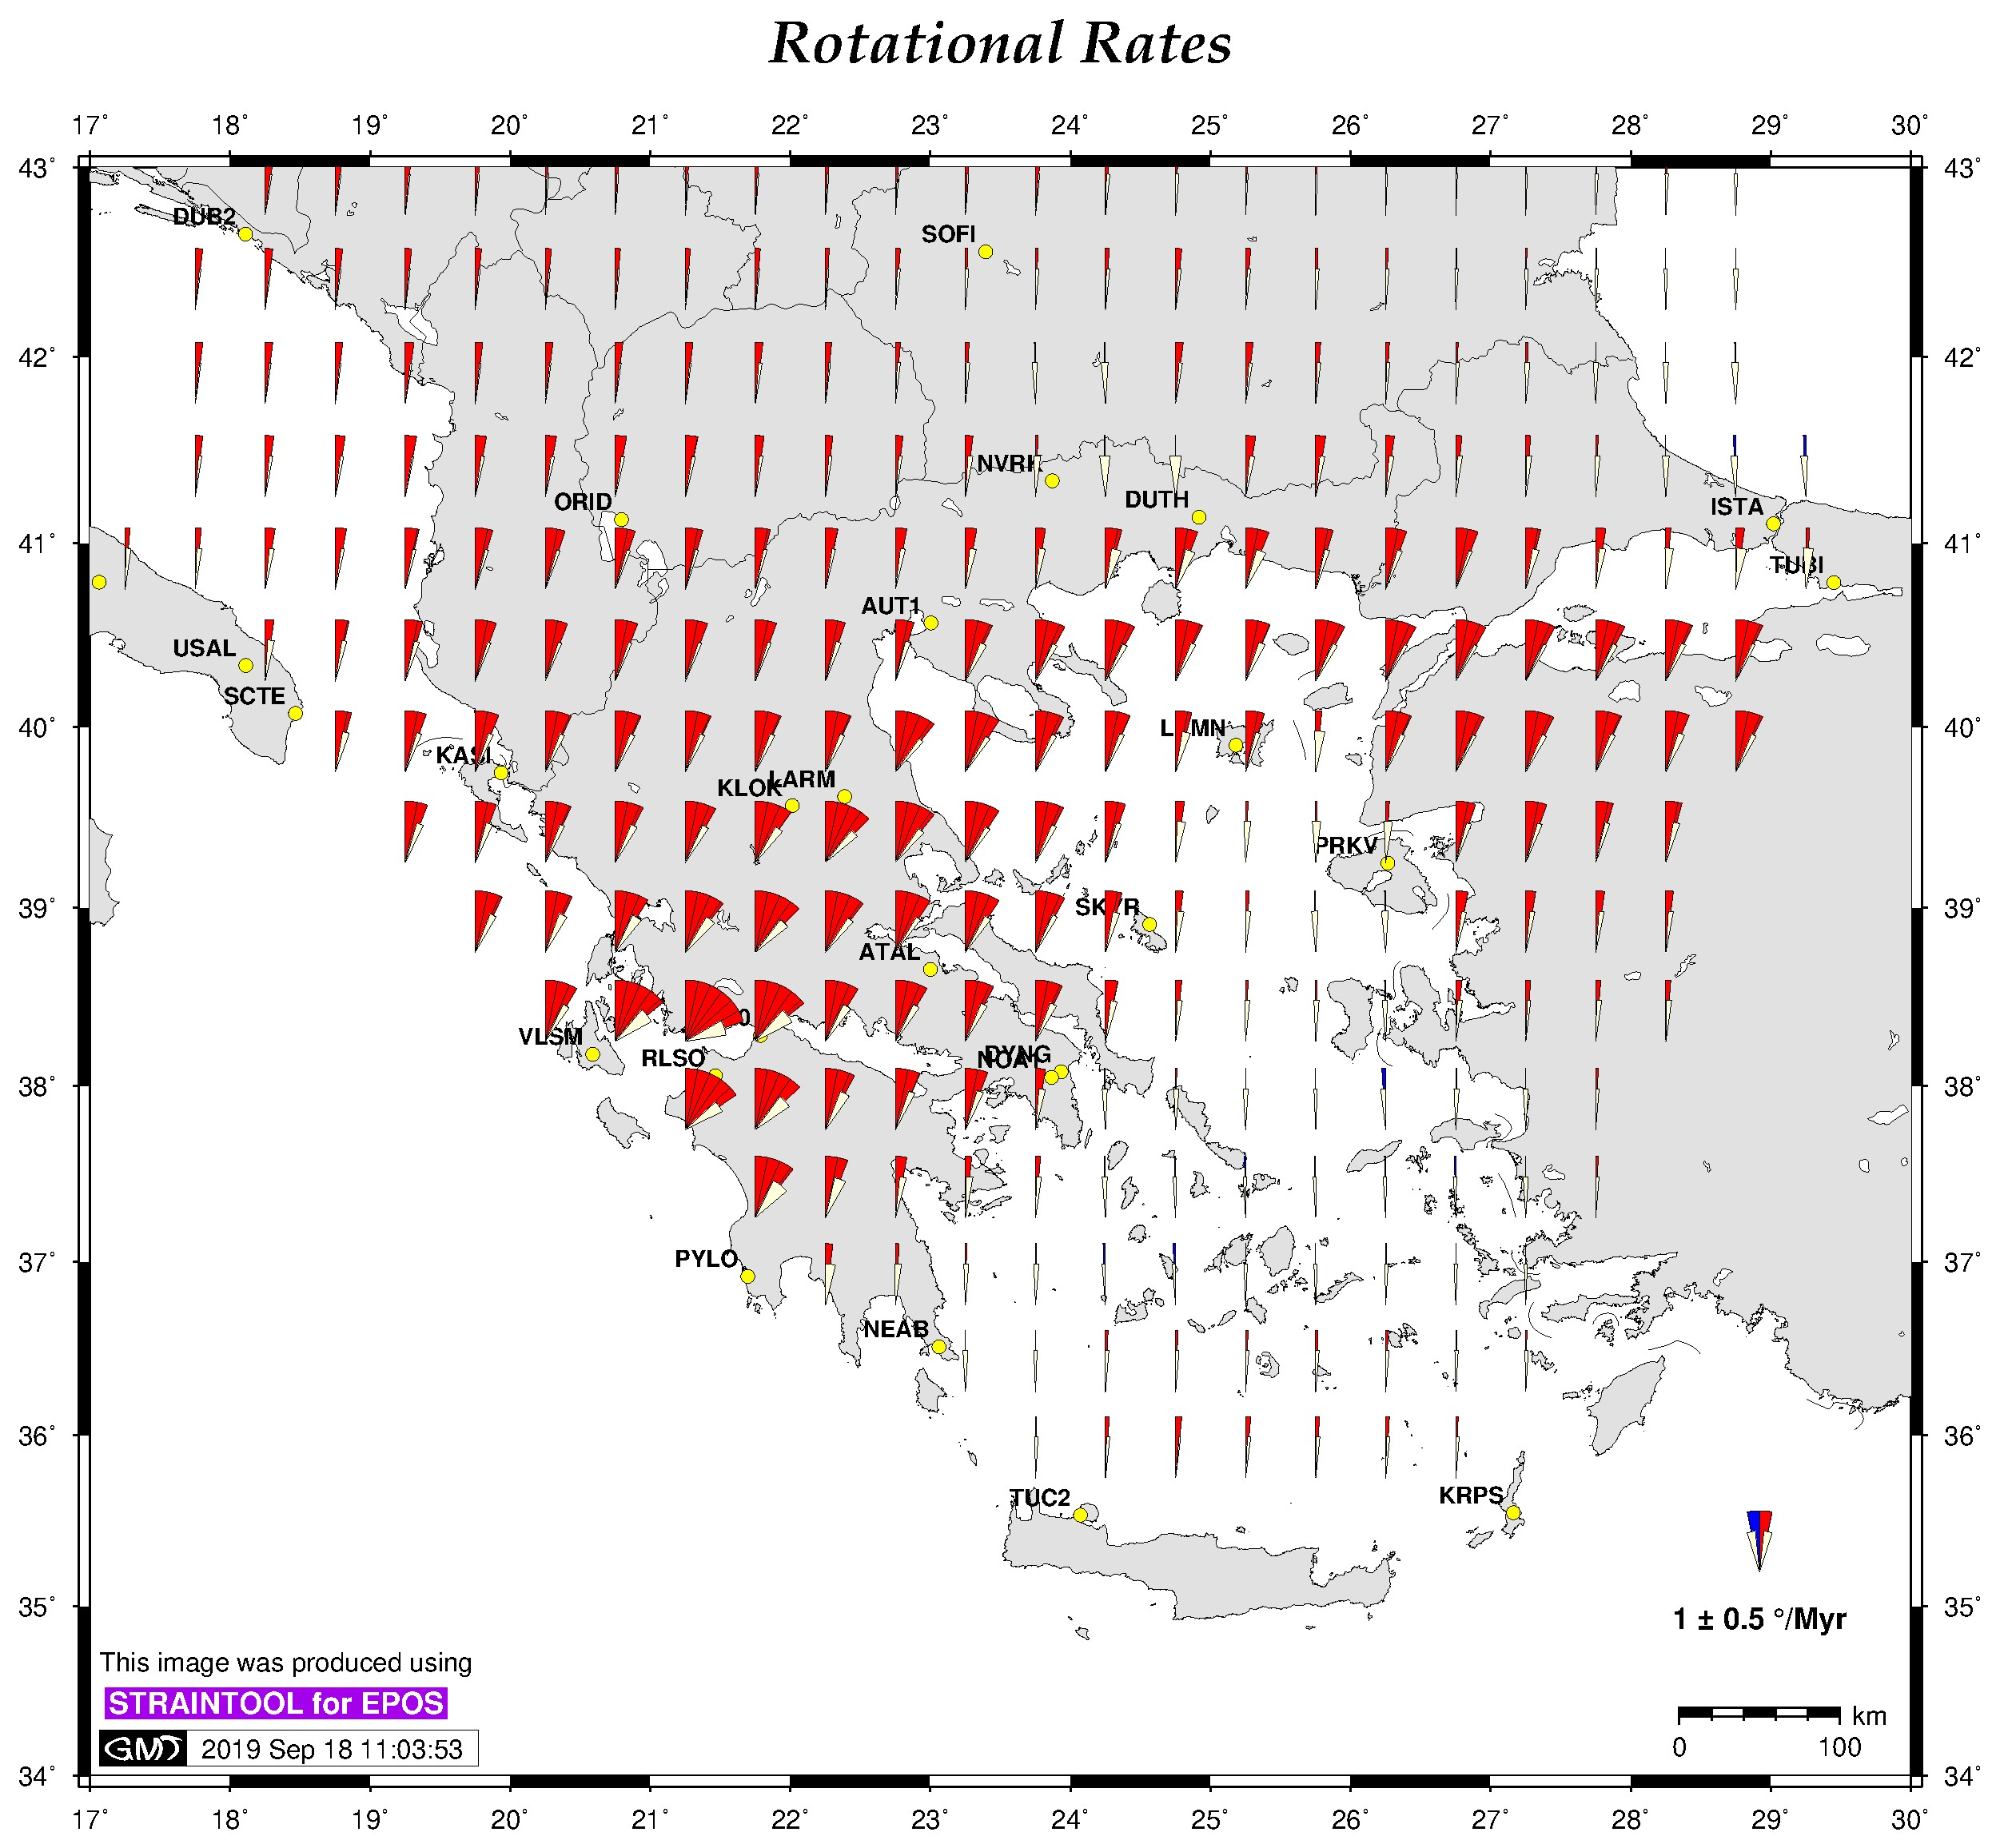
\includegraphics[width=0.9\textwidth]{grmidas-output_rot.jpg}     
    \end{center}
    \end{column}
  \end{columns}

\end{frame}
\note{}

\begin{frame}
 \frametitle{Strain Analysis}
 \framesubtitle{Greece region}
 \label{ch4:}
   
  \begin{columns}
    \begin{column}{0.5\textwidth}
      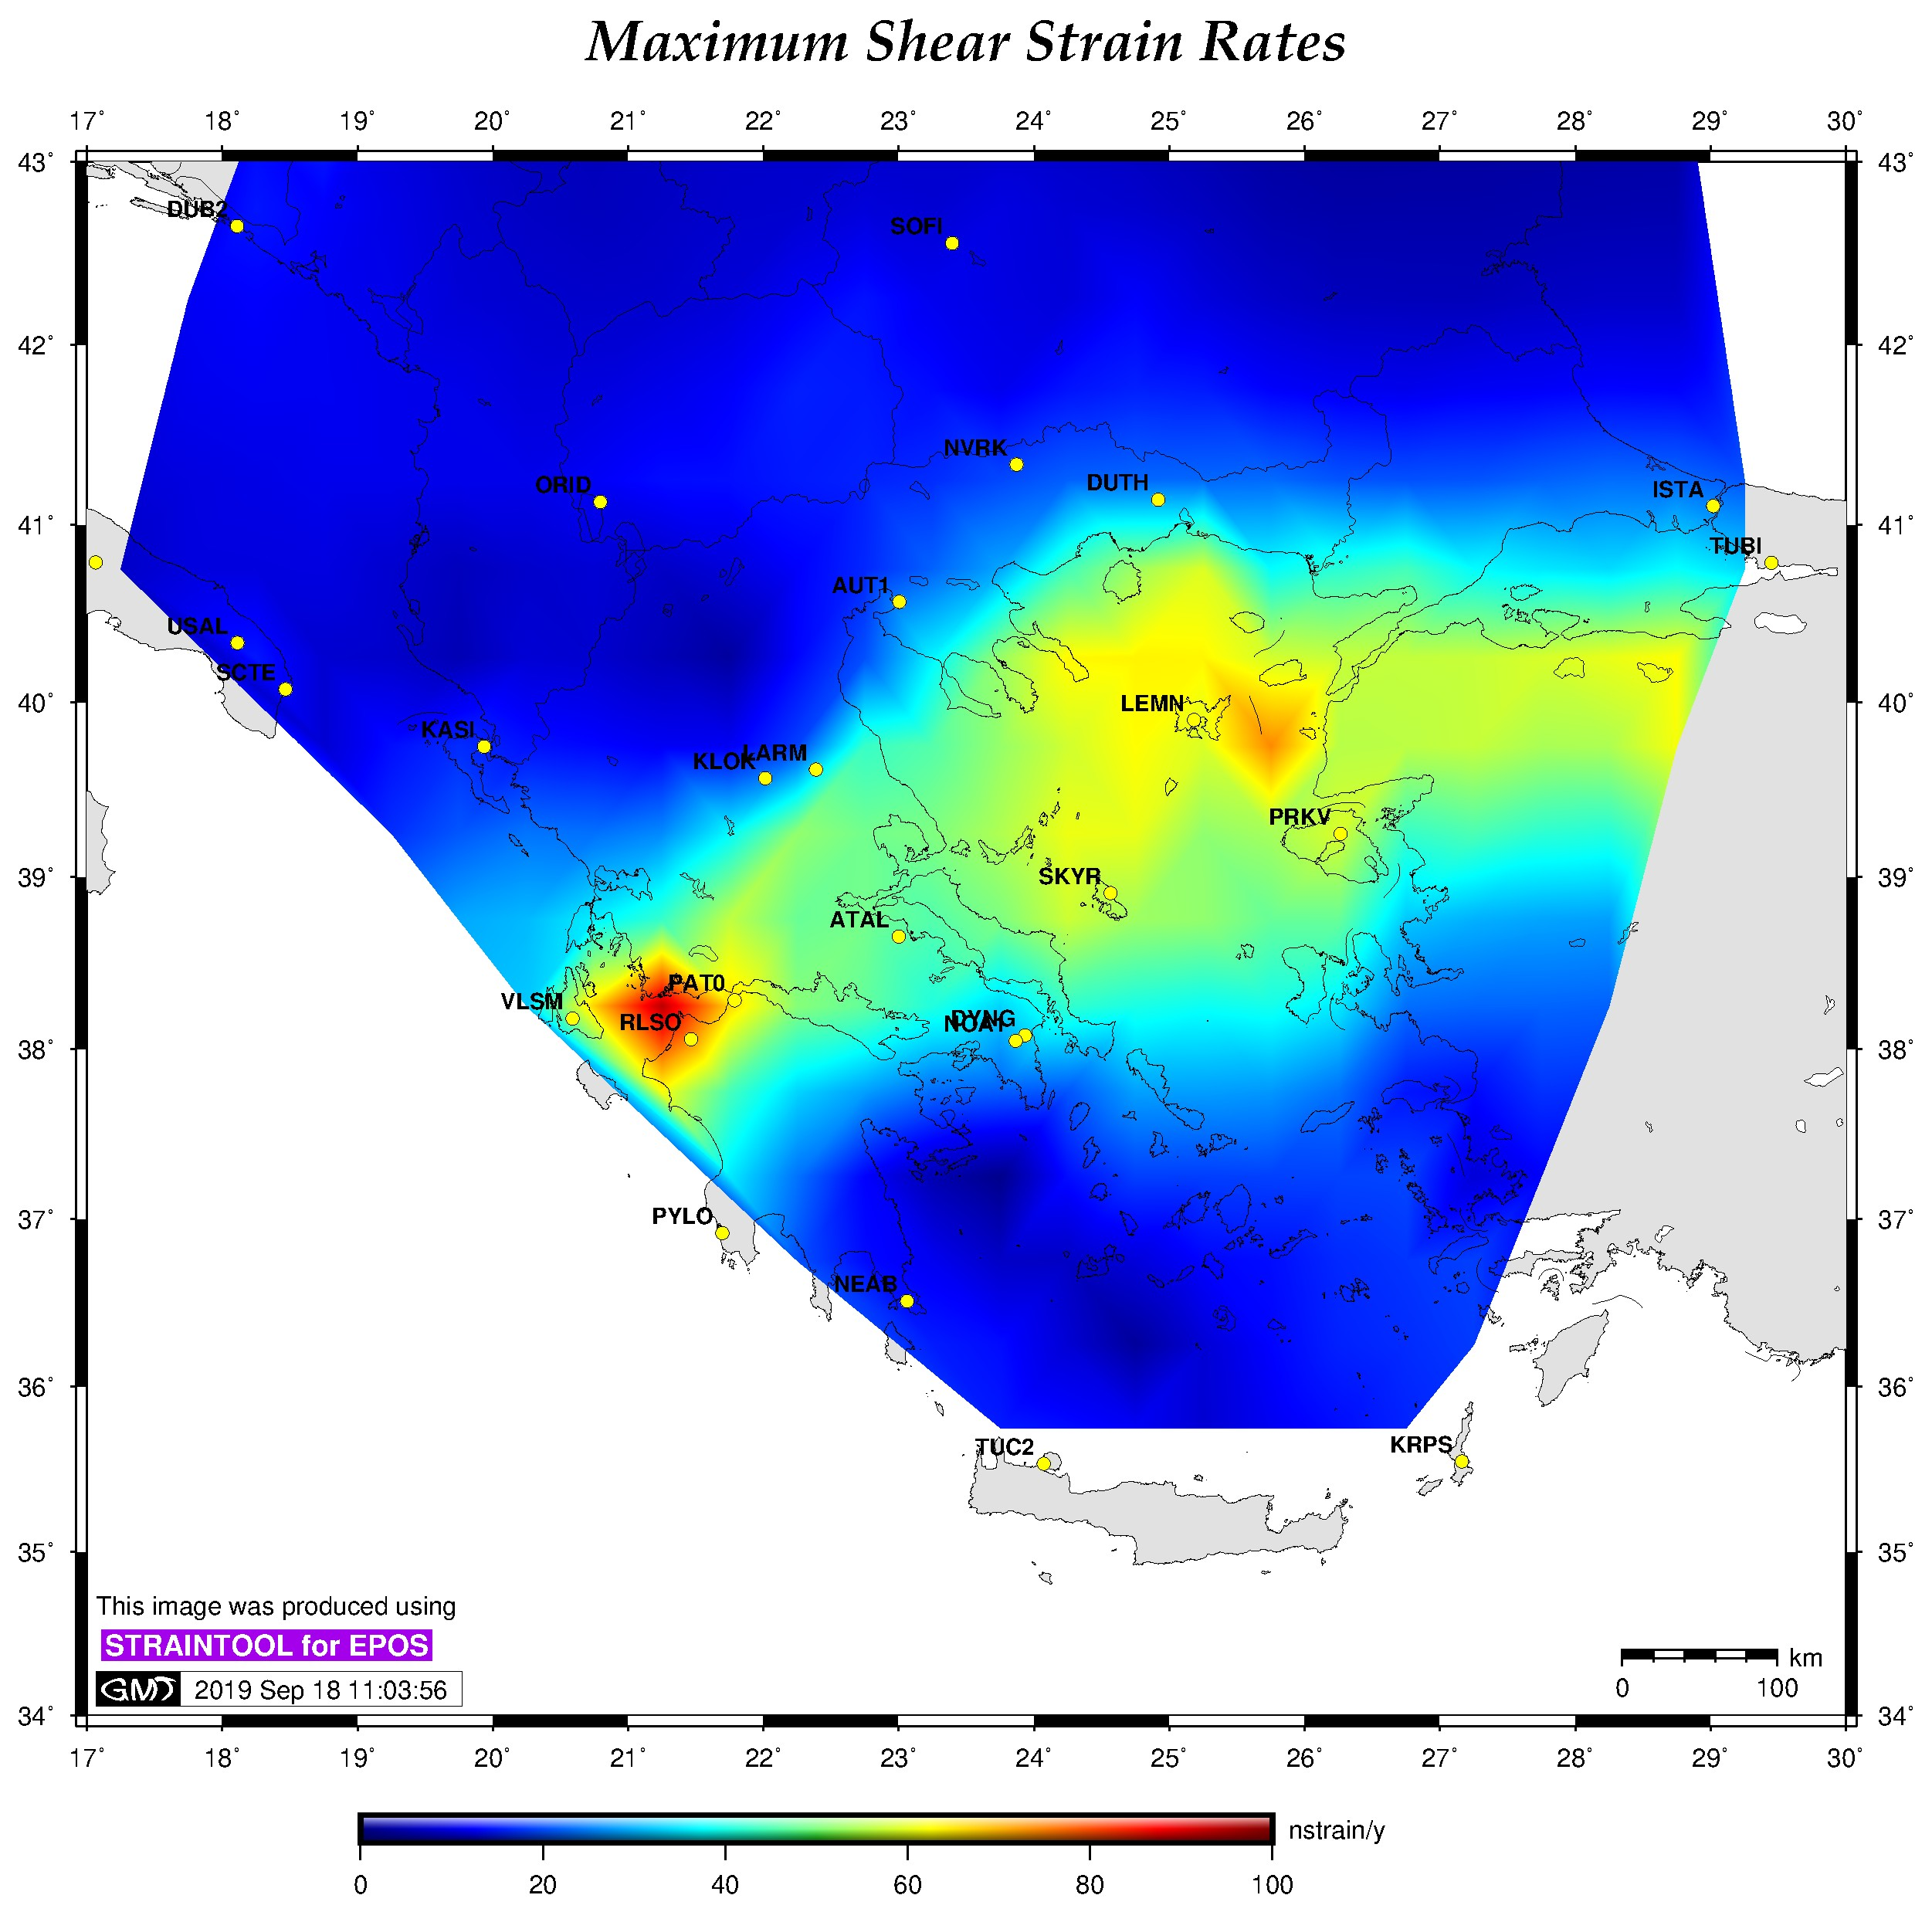
\includegraphics[width=.9\textwidth]{grmidas-output_gtot.jpg}   
    \end{column}
    \begin{column}{0.5\textwidth}
    \begin{center}
      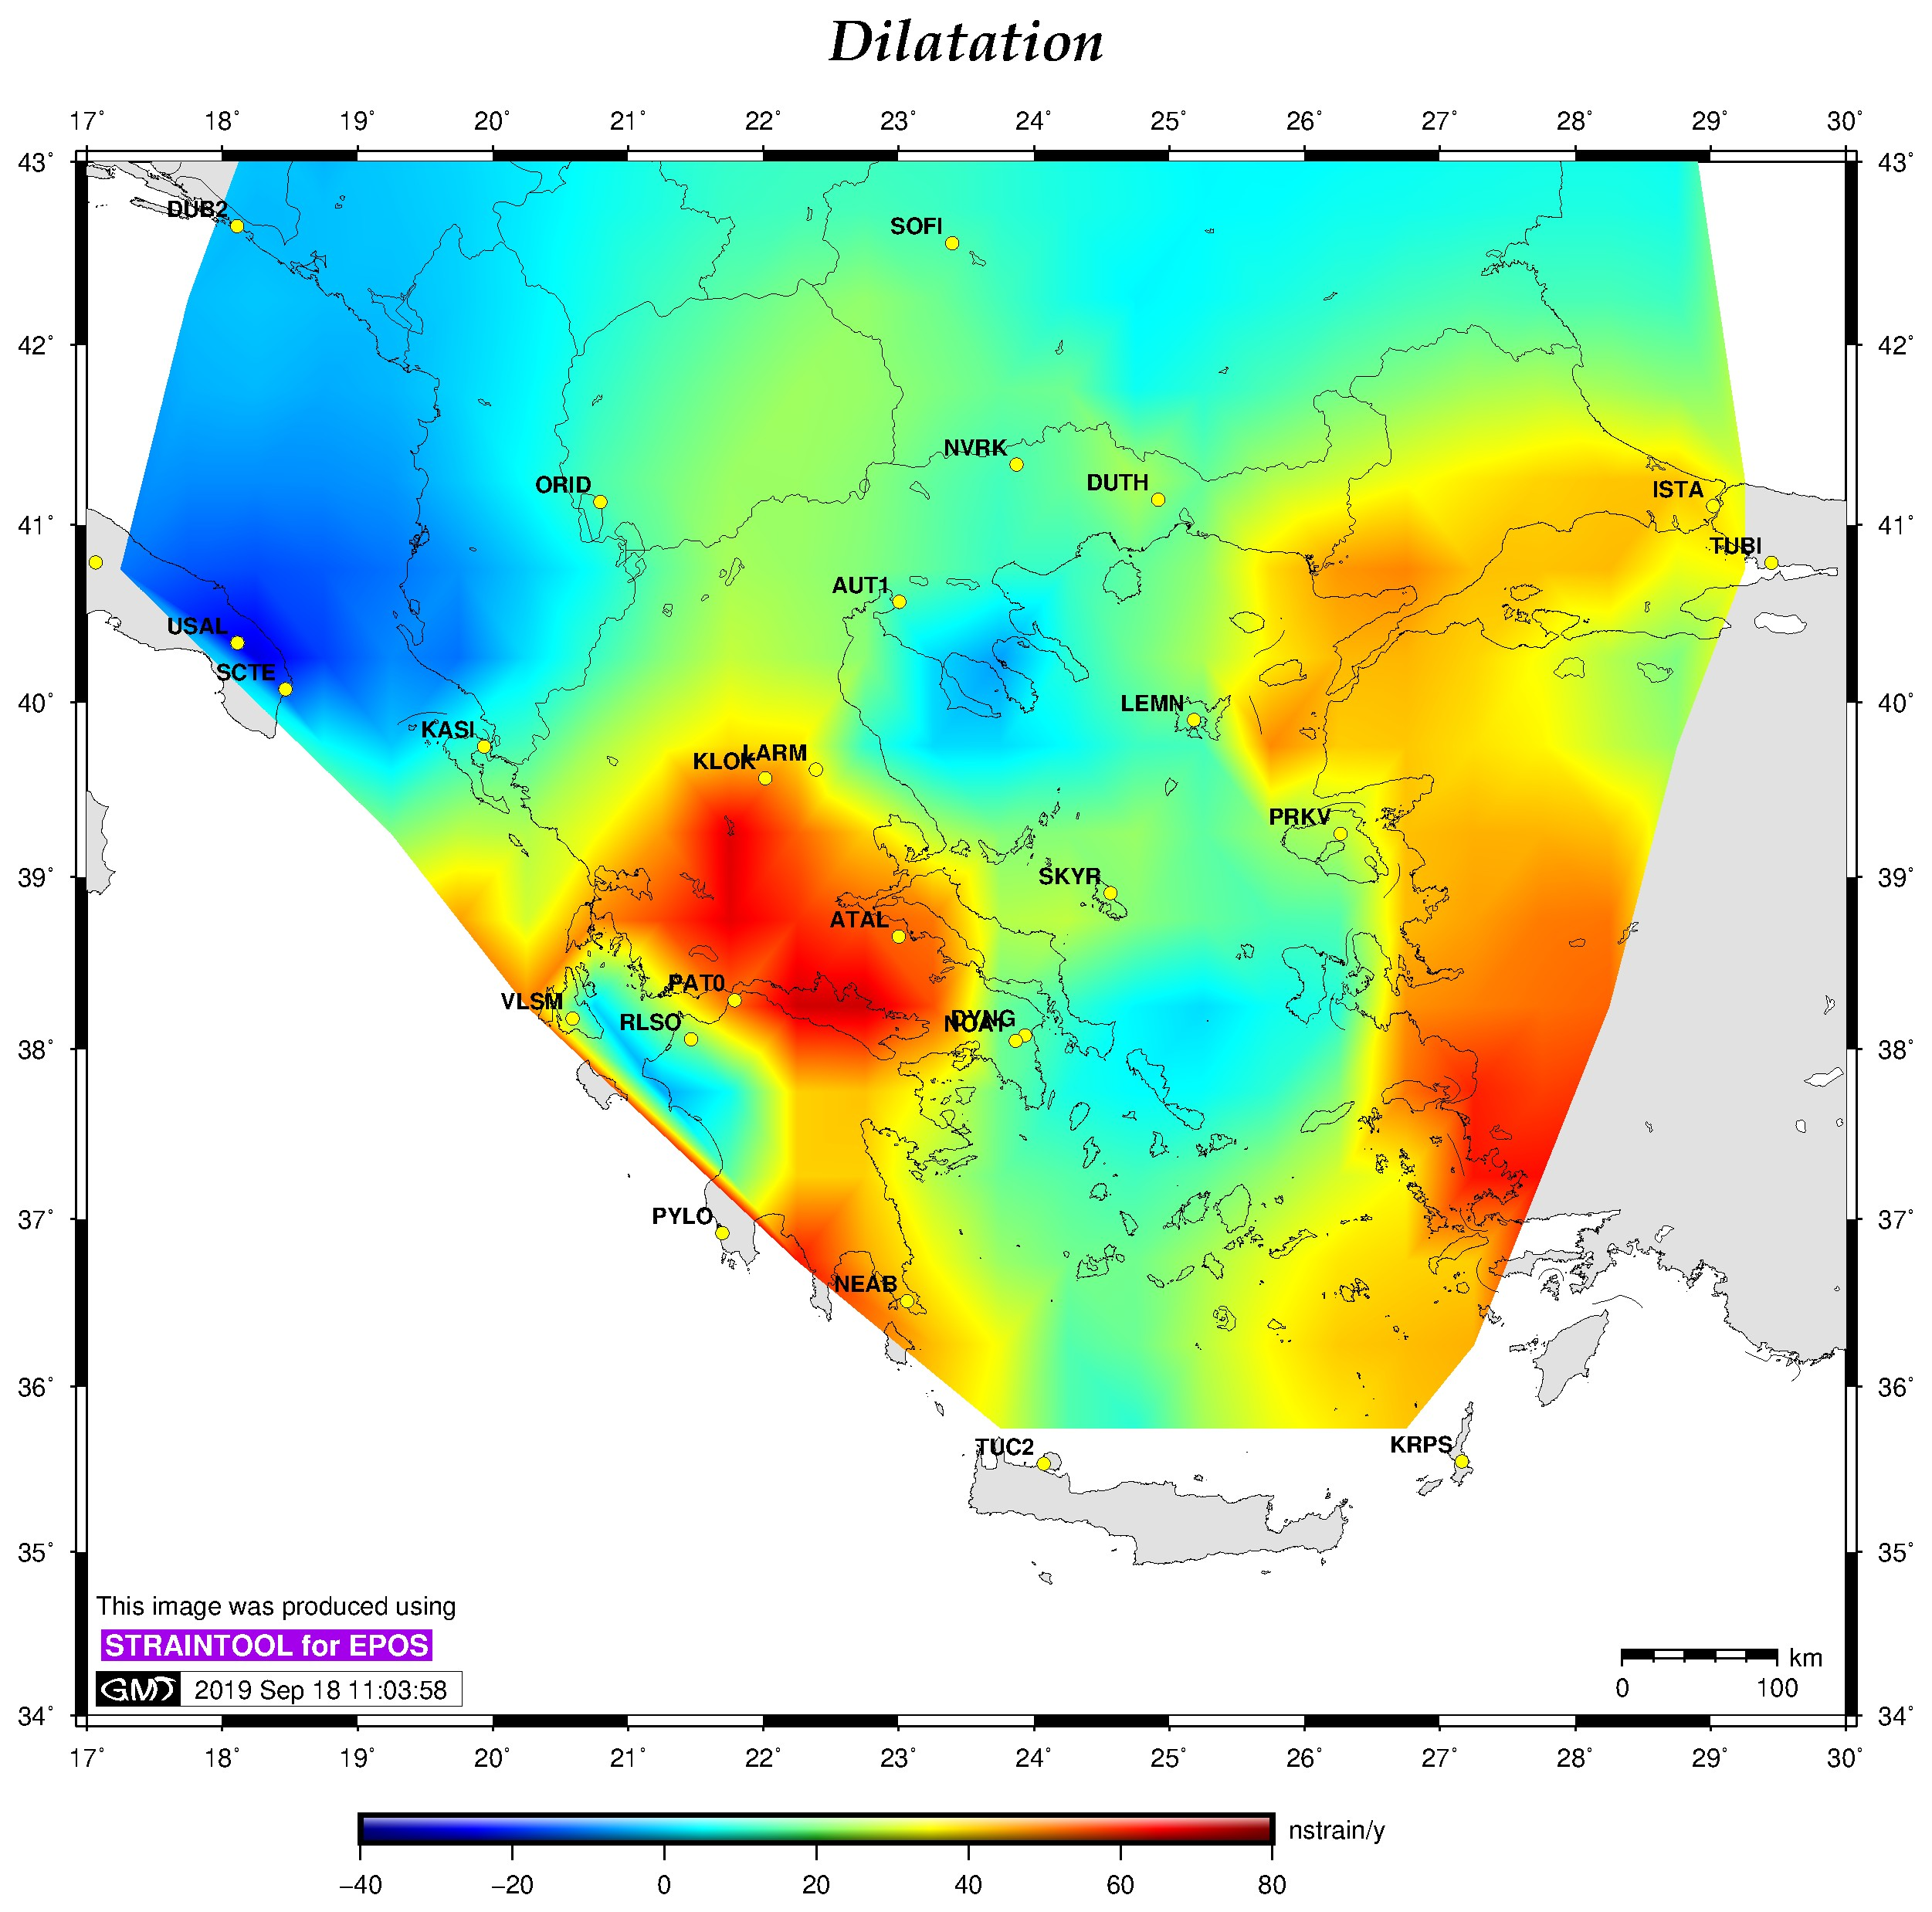
\includegraphics[width=0.9\textwidth]{grmidas-output_dil.jpg}     
    \end{center}
    \end{column}
  
  \end{columns}

\end{frame}
\note{}


\begin{frame}
 \frametitle{Strain Analysis}
 \framesubtitle{Greece region}
 \label{ch4:}
   
  \begin{columns}
    \begin{column}{0.5\textwidth}
      
      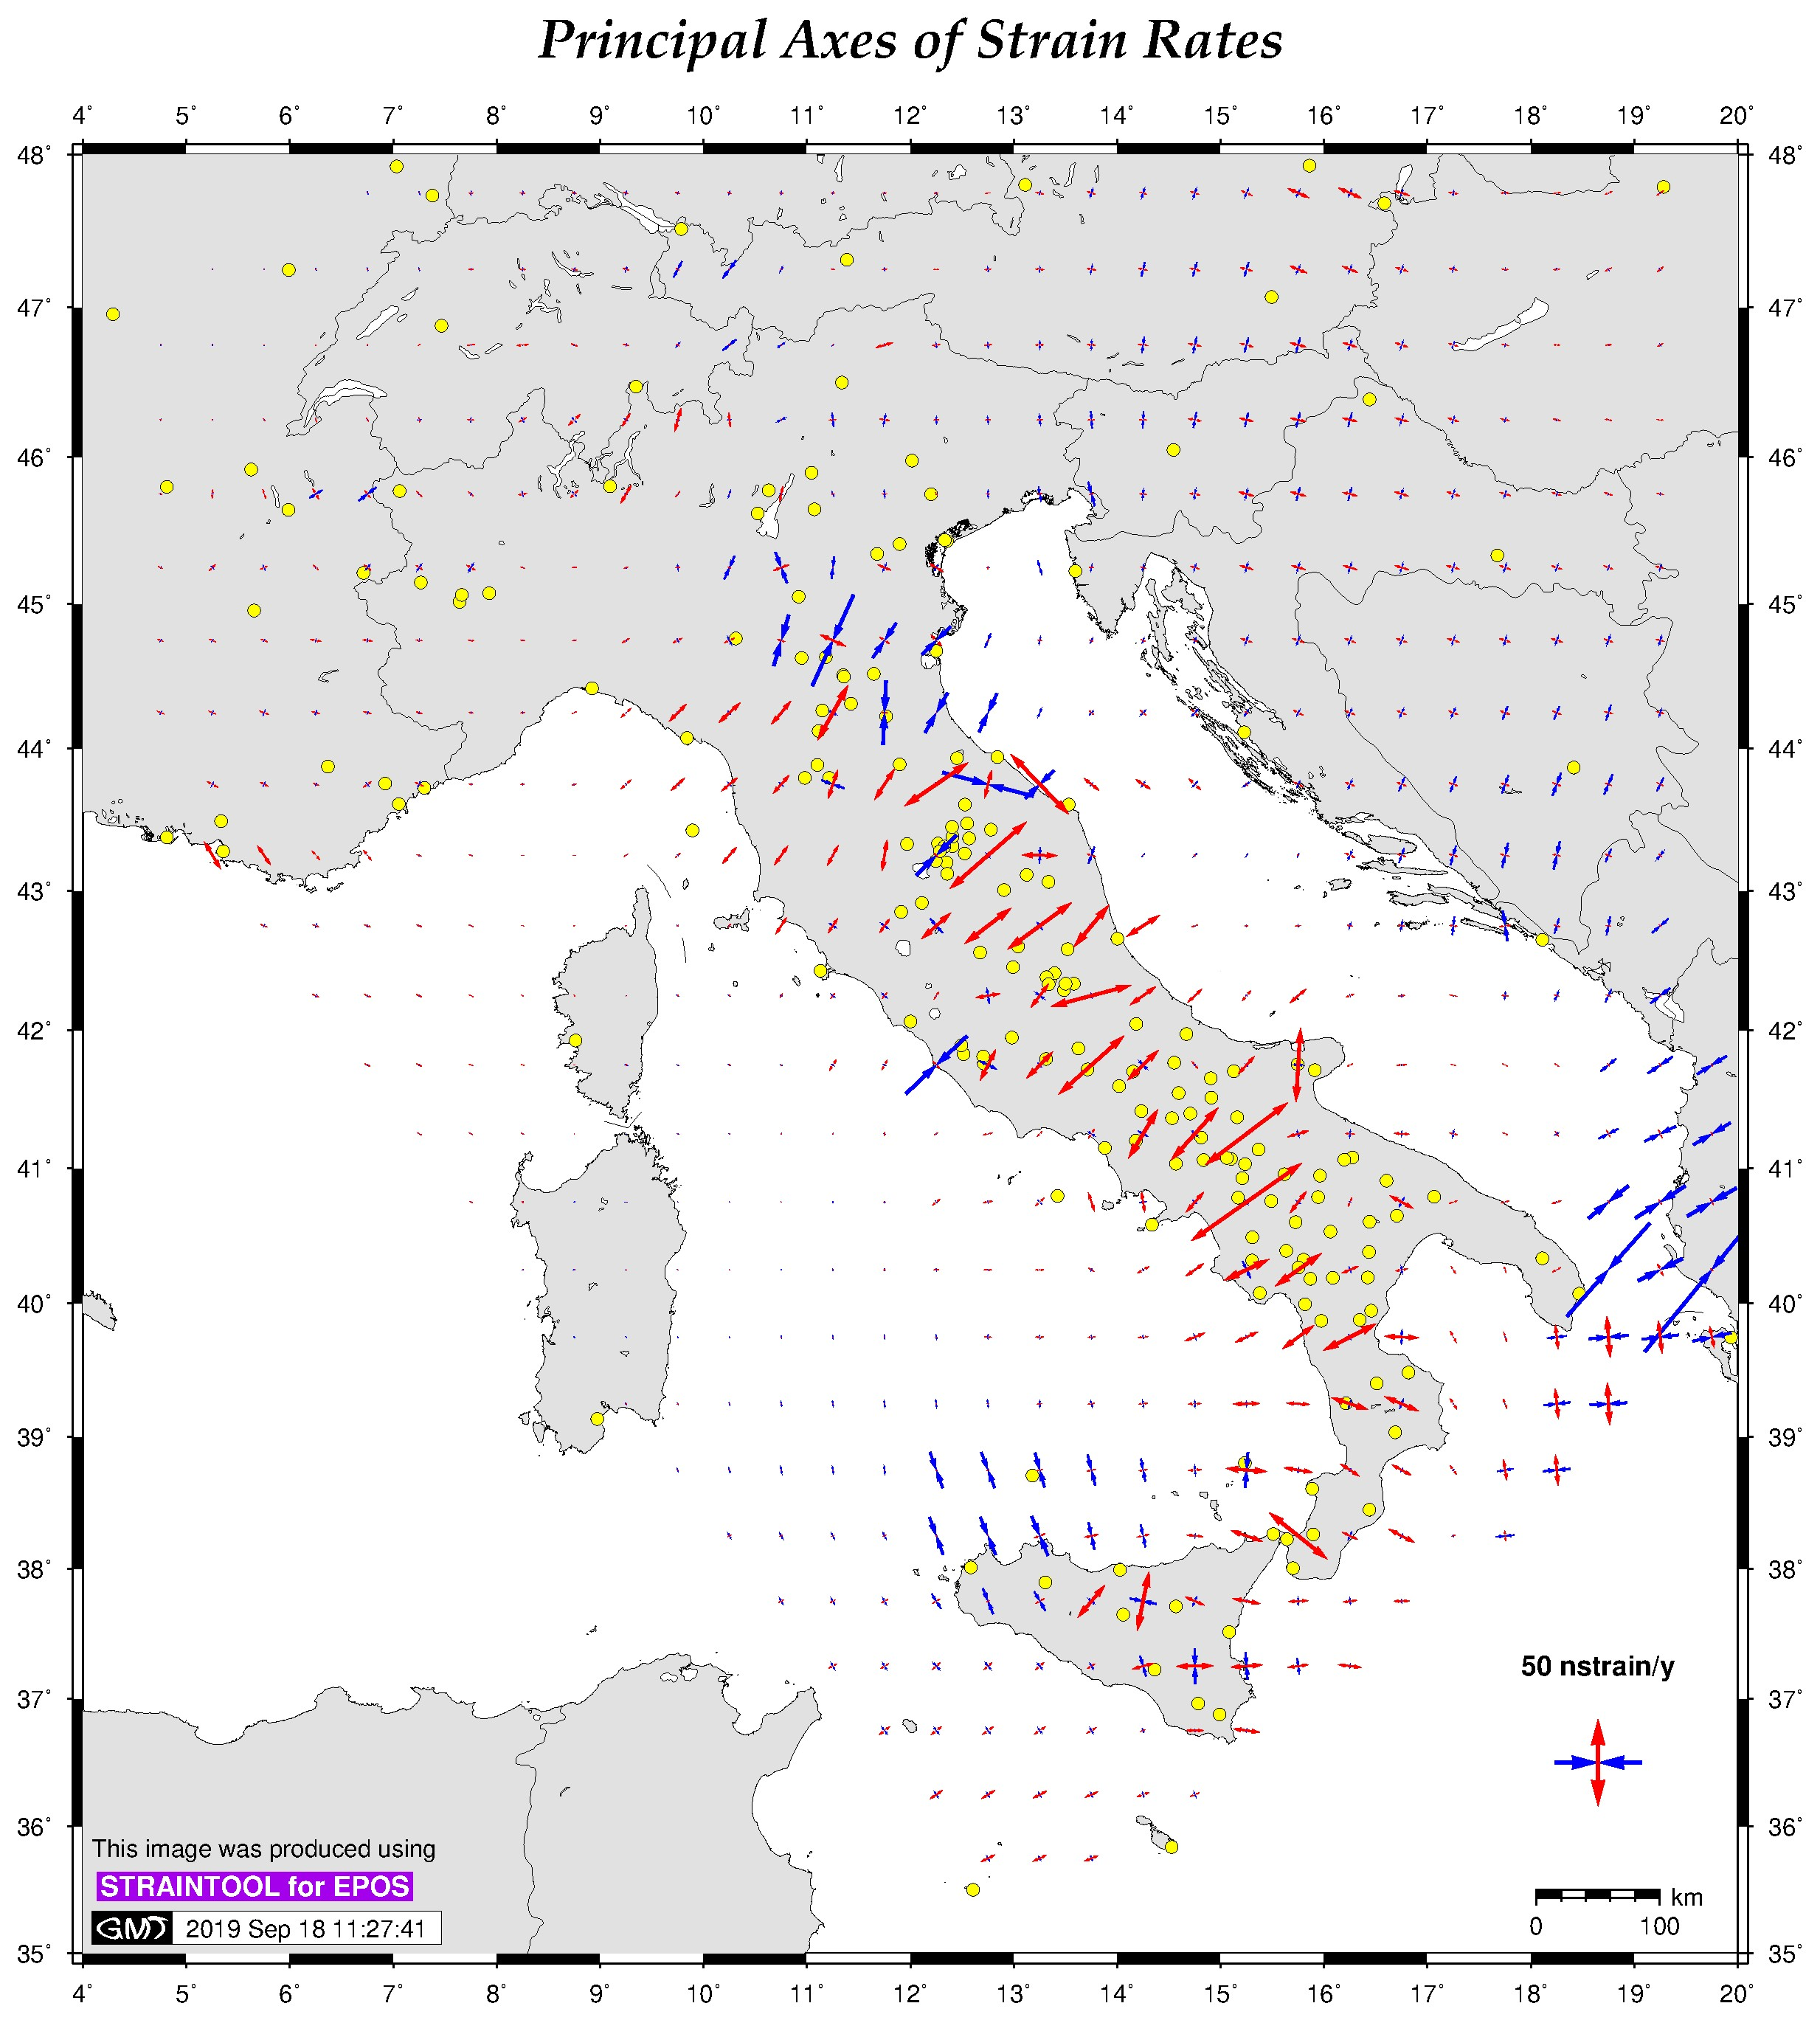
\includegraphics[width=.9\textwidth]{itmidas-output_str.jpg}   
    \end{column}
    \begin{column}{0.5\textwidth}
    \begin{center}
      
      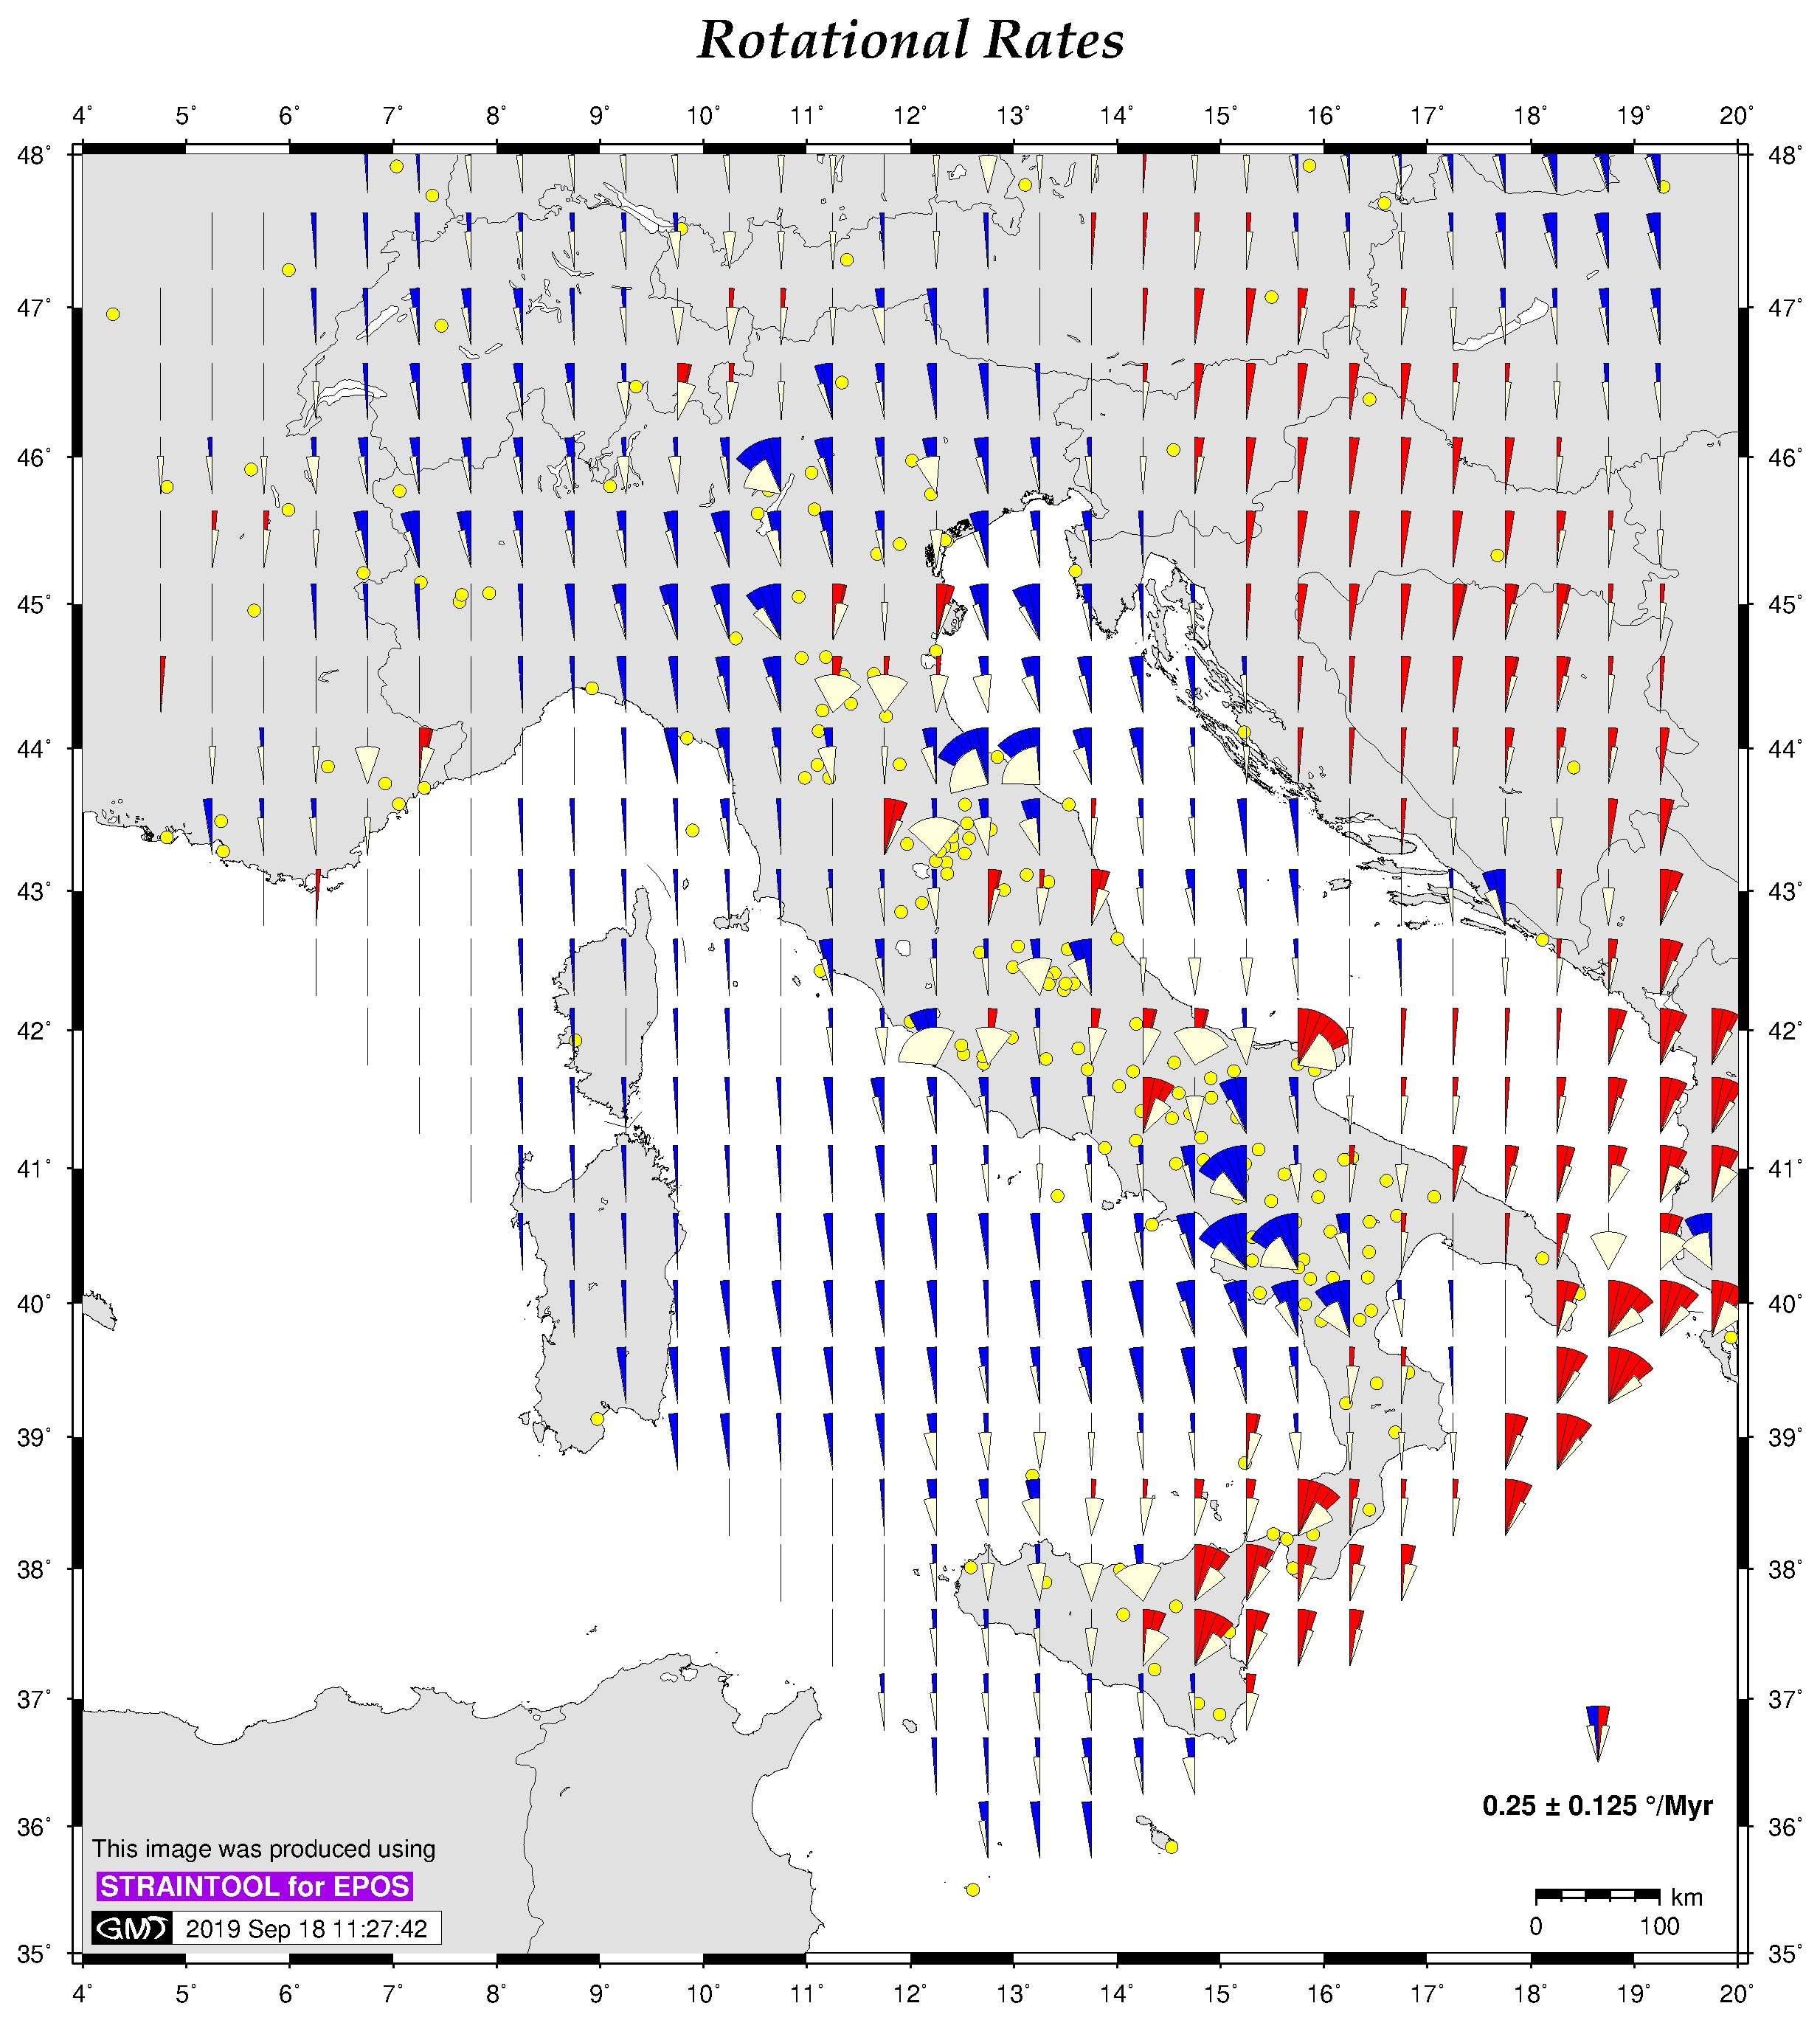
\includegraphics[width=0.9\textwidth]{itmidas-output_rot.jpg}     
    \end{center}
    \end{column}
  \end{columns}

\end{frame}
\note{}

\begin{frame}
 \frametitle{Strain Analysis}
 \framesubtitle{Greece region}
 \label{ch4:}
   
  \begin{columns}
    \begin{column}{0.5\textwidth}
      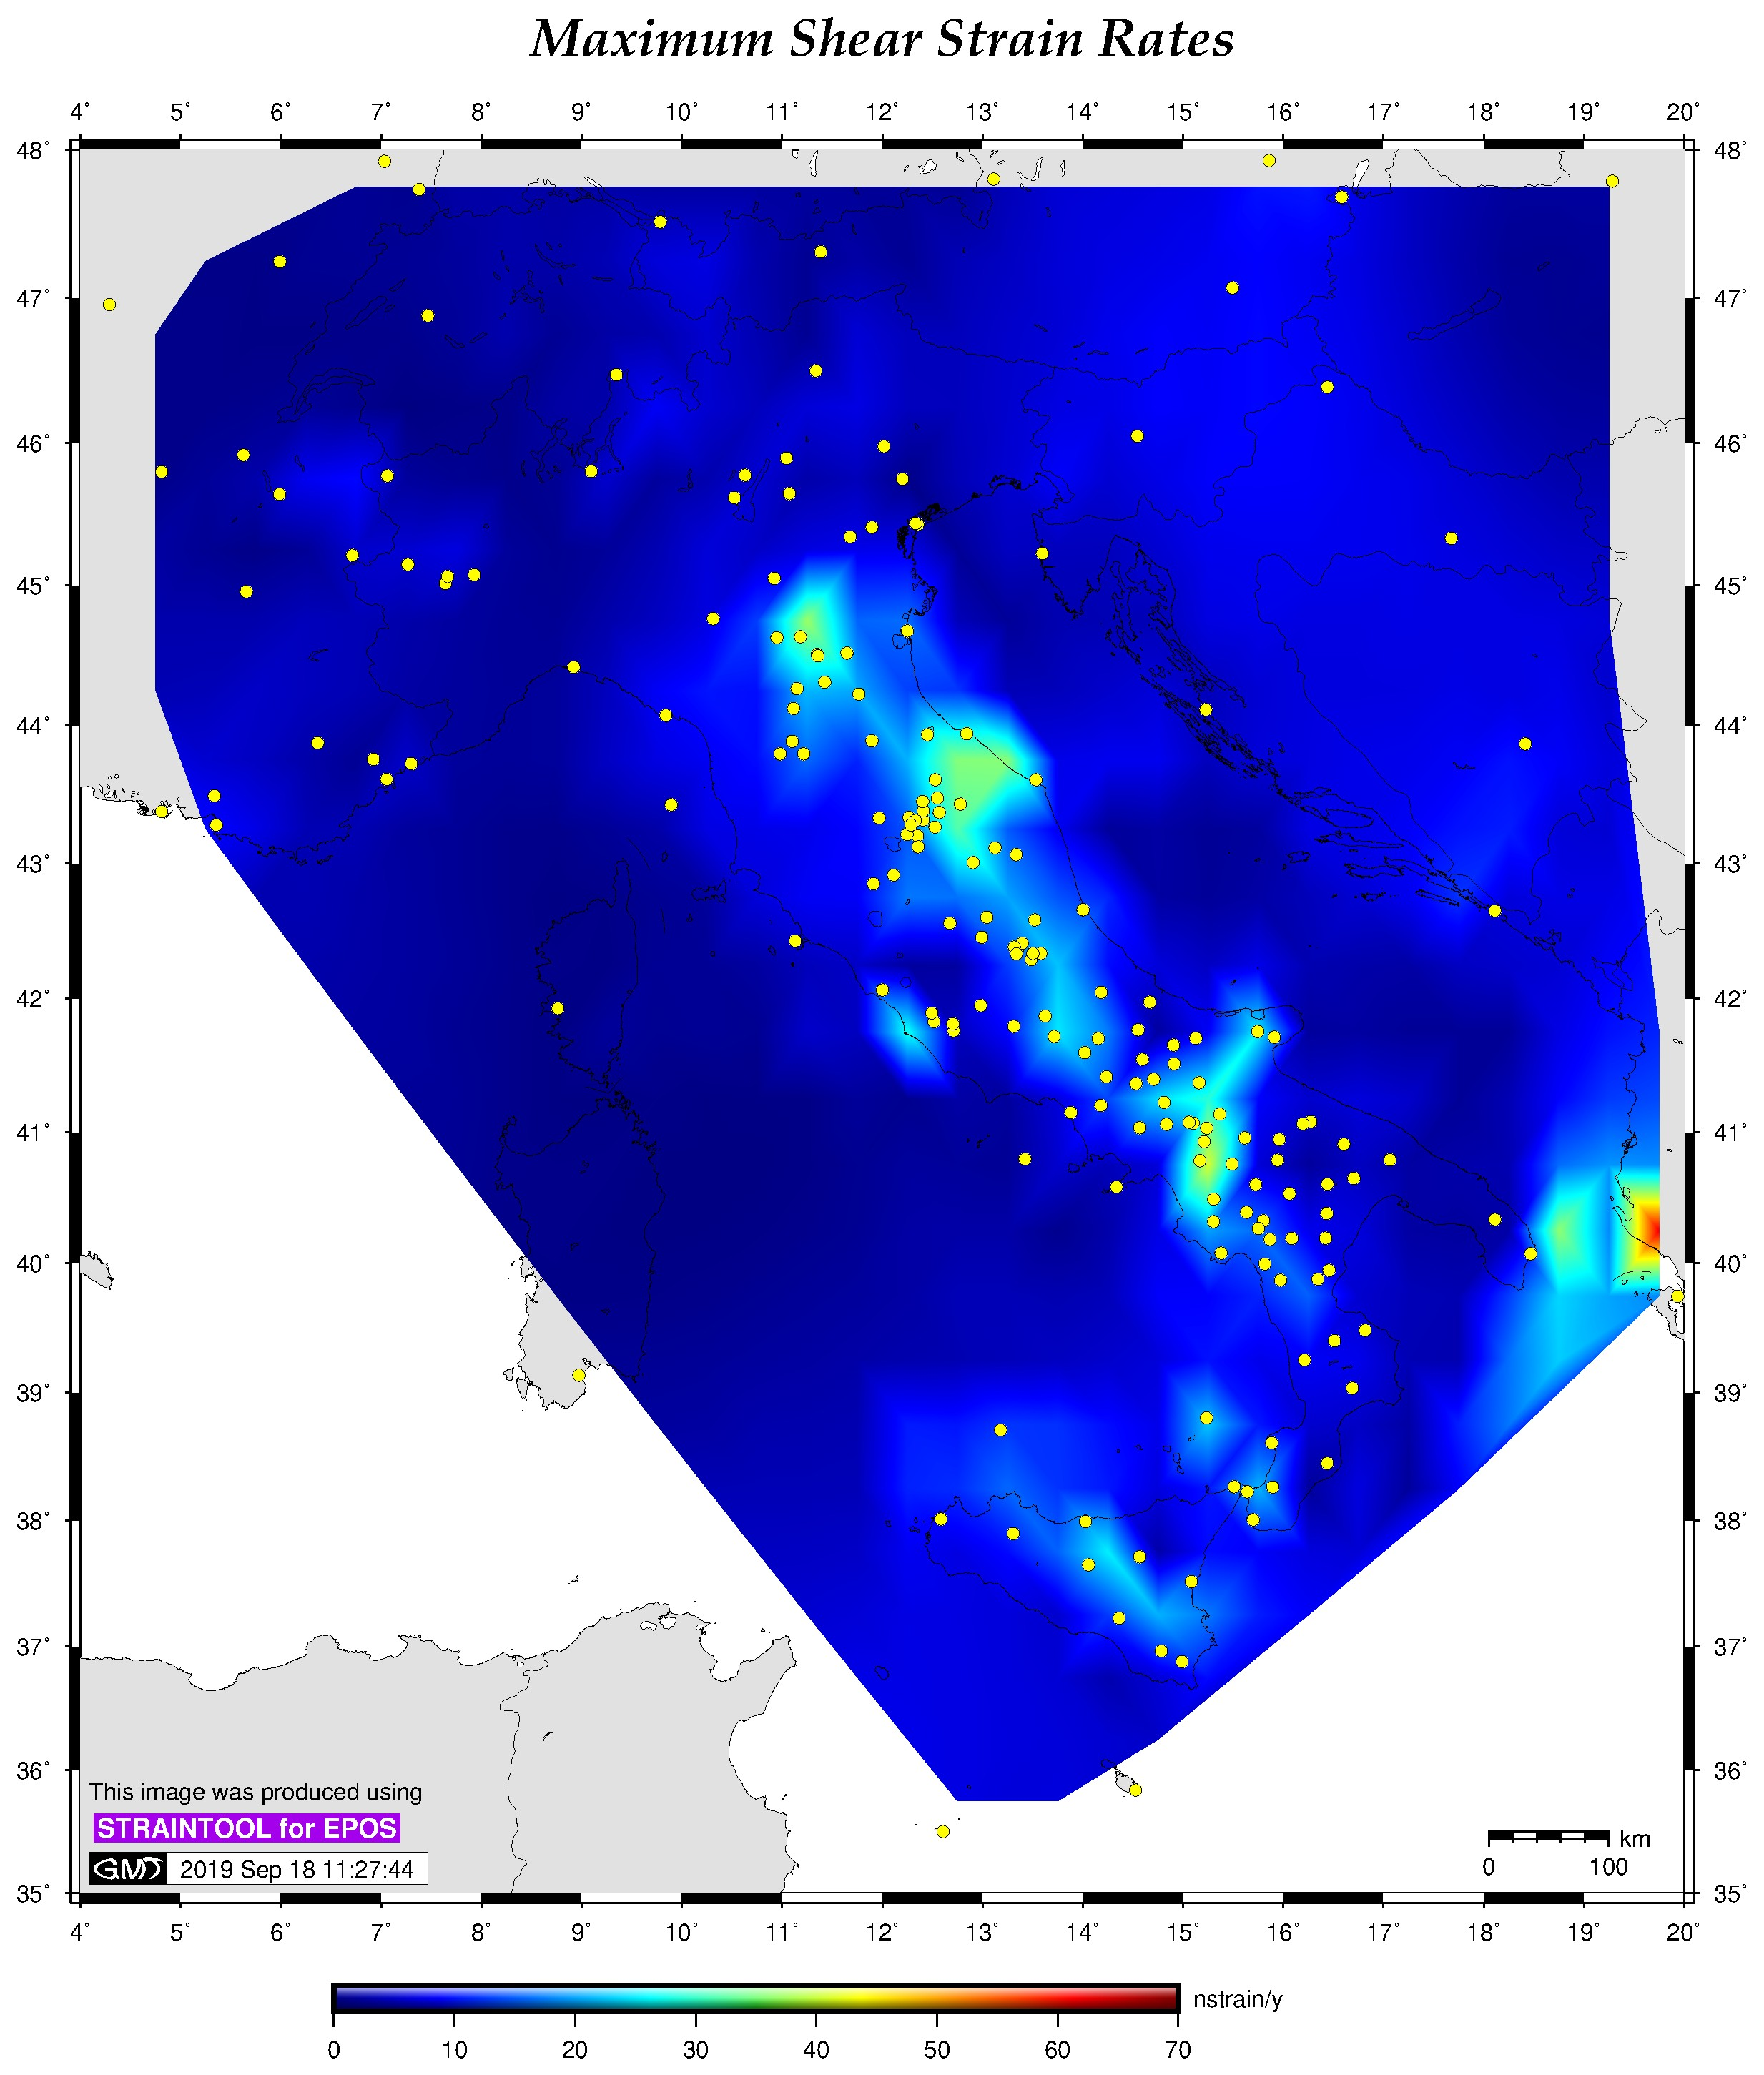
\includegraphics[width=.9\textwidth]{itmidas-output_gtot.jpg}   
    \end{column}
    \begin{column}{0.5\textwidth}
    \begin{center}
      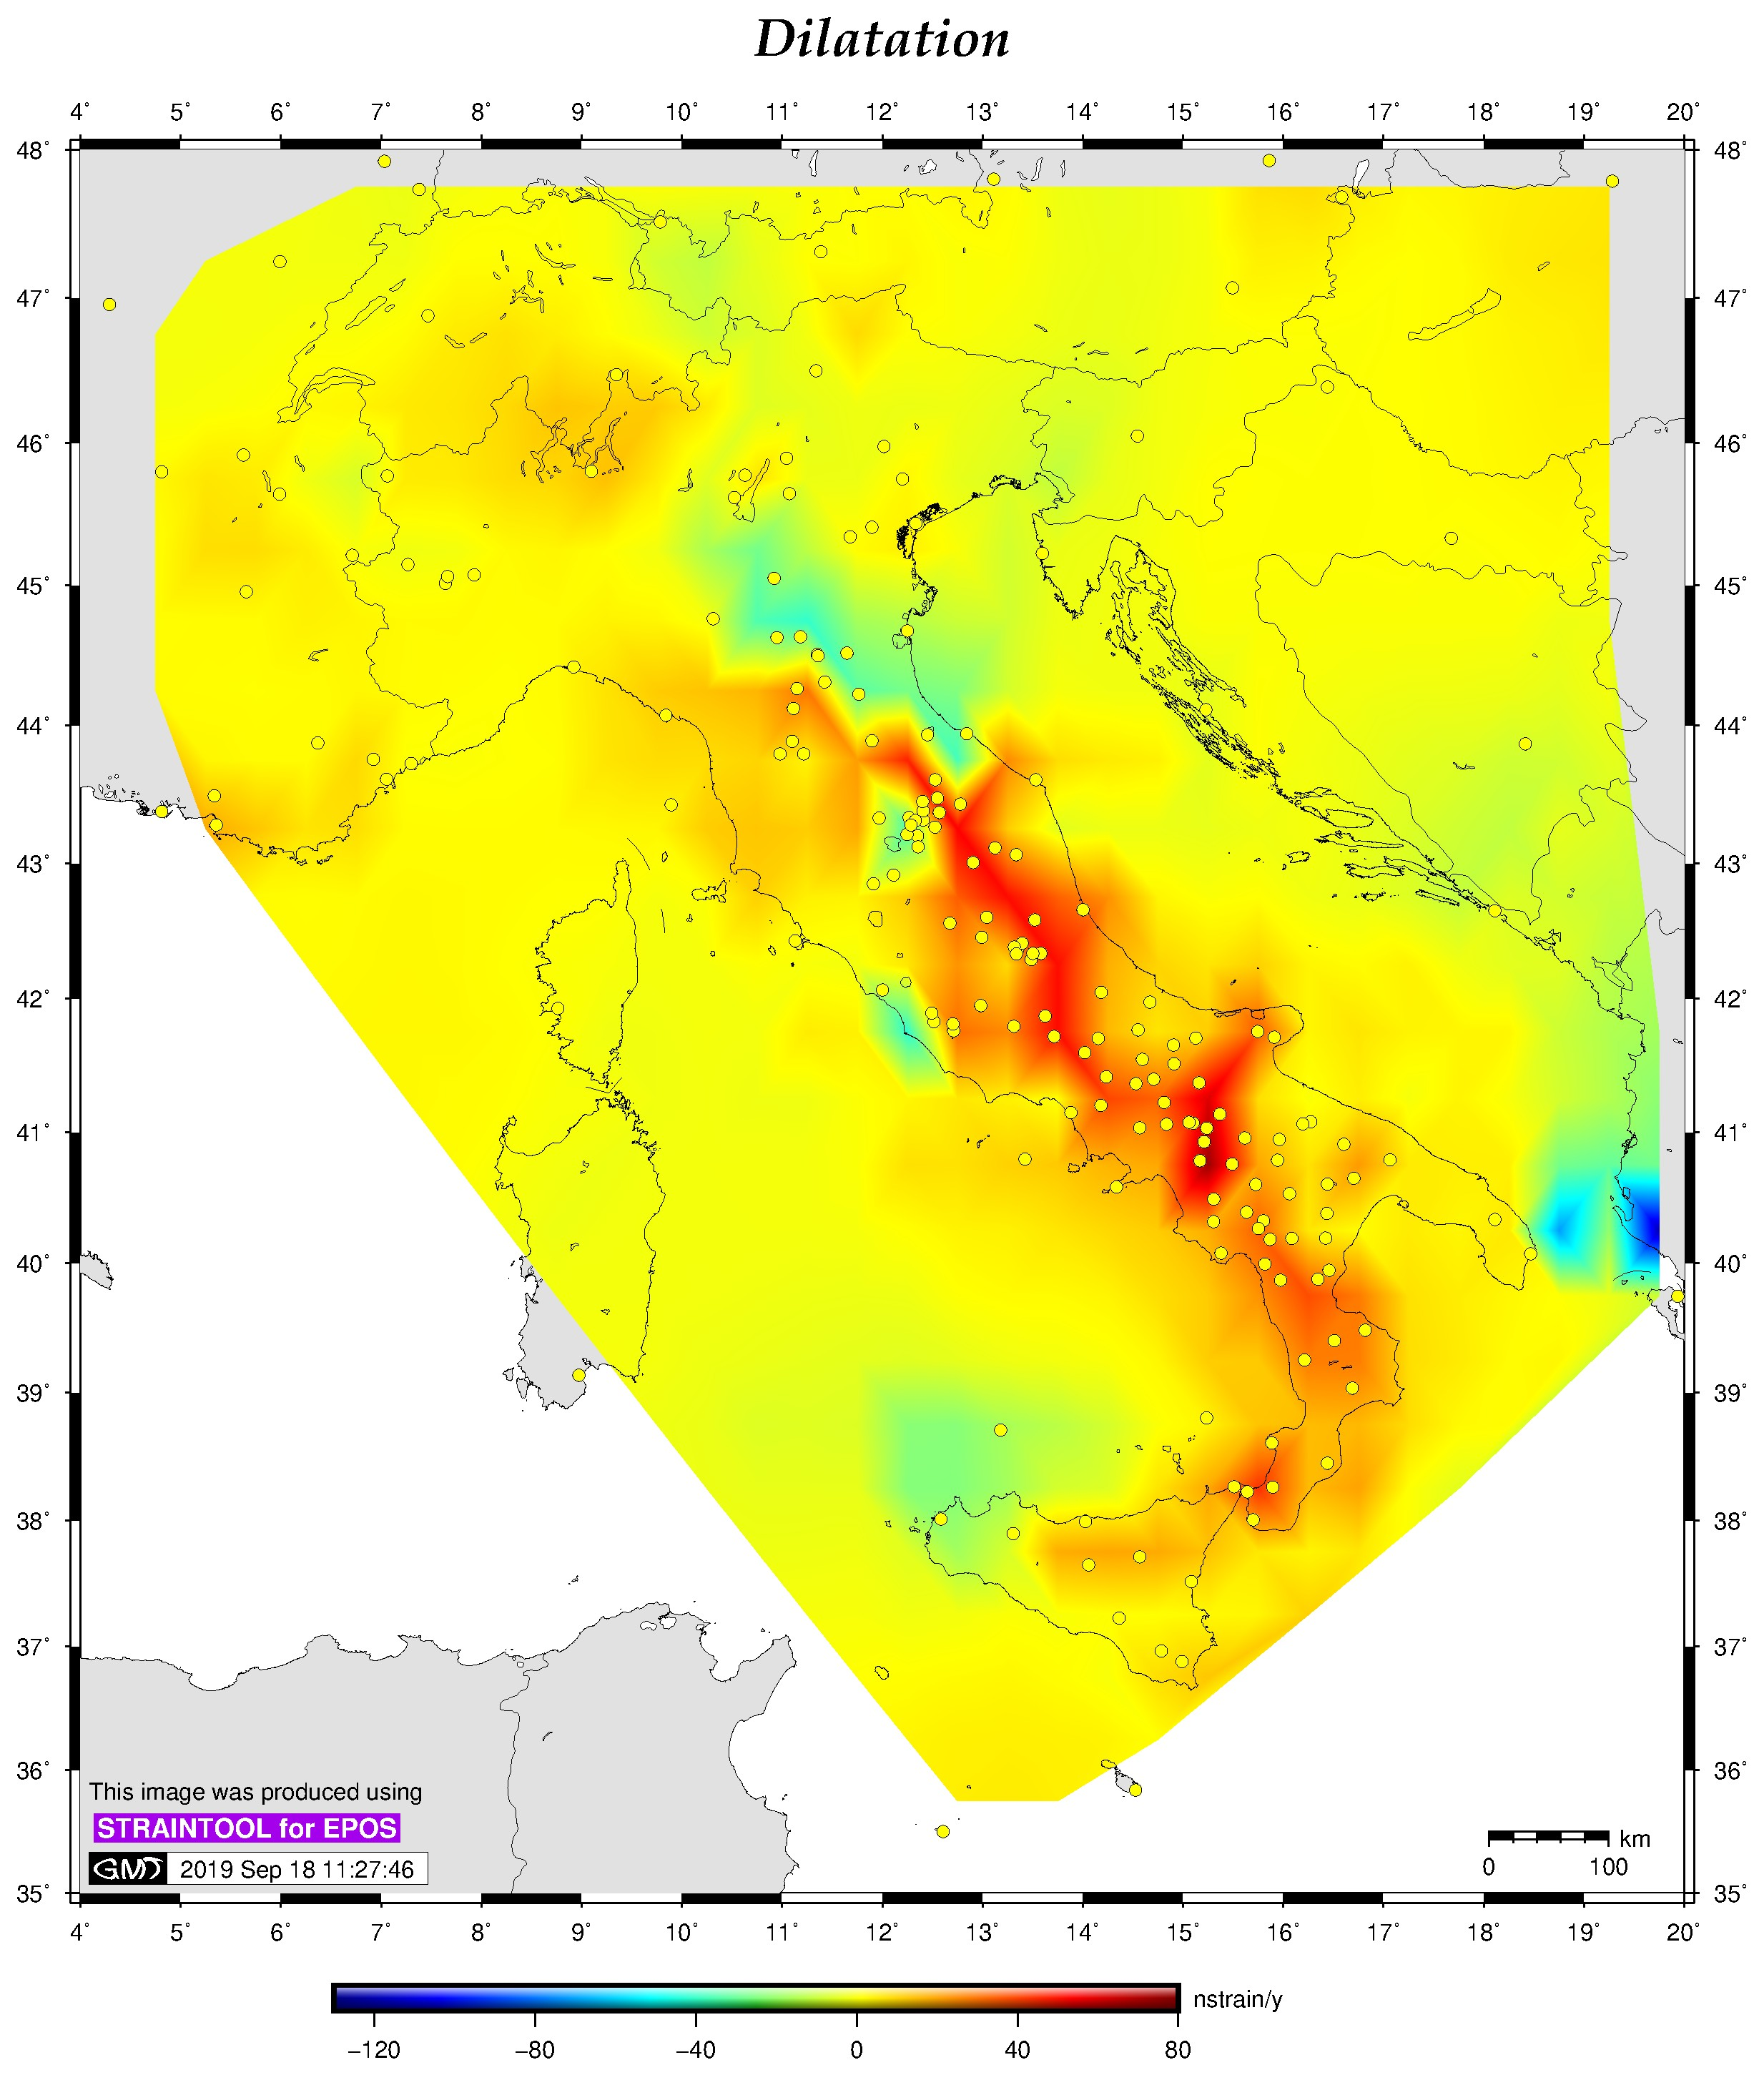
\includegraphics[width=0.9\textwidth]{itmidas-output_dil.jpg}     
    \end{center}
    \end{column}
  
  \end{columns}

\end{frame}
\note{}



%\begin{frame}
%  \frametitle{}
%  \framesubtitle{}
%  \label{ch4:}

%\end{frame}
%\note{}

% \section{Conclusions}
 
% \graphicspath{Figs/}

\begin{frame}
 \frametitle{Conclusions}
 \framesubtitle{StrainTool open-source software v1.0}
 \label{ch5:concl}
  
  \begin{itemize}
    \item We propose a new, open-source tool to estimate strain in geodesy and geodynamics, the \texttt{STRAINTOOL}
    \item Free, flexible and cross-platform-compatibility.
    \item Use different algorithms to estimate strain tensor parameters.
    \item We validated our calculations using two open-source algorithms recommended by EPOS-IP, namely the VISR and STIB as well as the SSPX software suite.
    \item Οur results reproduce the gross features of tectonic deformation in both Italy and Greece, such as NE-SW extension across the Apennines and N-S extension in Central Greece.
    \item It is anticipated that the significant increase of GNSS data amount associated with the operational phase of EPOS in the forthcoming years will be of great value to perform an unprecedented, reliable strain rate computation over the Eurasian plate.
  \end{itemize}
\end{frame}
\note{}


\begin{frame}
 \frametitle{Conclusions}
 \framesubtitle{Tectonic strain in Eurasia}
 \label{ch5:concl}
  \begin{itemize}
    \item
    \item NE-SW extension across the Apennines.
    \item N-S extension in Central Greece.
    \item NE-SW compression acrossthe area of Albania's shoreline.
  \end{itemize}

\end{frame}
\note{}

%\begin{frame}
%  \frametitle{}
%  \framesubtitle{}
%  \label{ch5:concl}

%\end{frame}
%\note{}

% \include{Chapter6/ch6pres}
% % \section{Δημοσιεύσεις  - Λογισμικό}

\begin{frame}
  \frametitle{Δημοσιευμένες εργασίες}
  \framesubtitle{}

  
\begin{scriptsize}
    \begin{itemize}
\item[\faFile] Anastasiou D., Chouliaras G., Papanikolaou X., Marinou A., Zacharis V., Galanis J., Drakatos G., Paradissis D. (2015) \textbf{Geodetic and seismological analysis of the January 26, 2014 Cephalonia Island earthquake sequence.}  \textit{26th General Assembly of the IUGG,Prague, Czech Republic, 22/6 - 2/7.}\\
  \item[\faFile] Ganas A., Marinou A., Anastasiou D., Paradissis D., Papazissi K., Tzavaras P. and Drakatos G. (2013). \textbf{GPS-derived estimates of crustal deformation in the central and North Ionian Sea, Greece: 3-yr results from NOANET continuous network data.} \textit{Journal of Geodynamics 67, Pages 62–71A, DOI:\url{10.1016/j.jog.2012.05.010}}\\
    \item[\faFile] Papazissi K., Anastasiou D., Marinou A., Mitsakaki C., Papanikolaou X., Paradissis D. (2010) \textbf{Deformation studies in the Gulf of Patras, Western Greece.} \textit{Honorary Volume in honor of D.Arabelo, Professor of the Aristotle University of Thessaloniki.}\\
    \item[\faFile] Anastasiou D., Marinou A., Mitsakaki C., Papazissi K., Papanikolaou X., Paradissis D. (2010). \textbf{Crustal Deformation in the Patras Gulf, Greece, from GPS Data Analysis.} \textit{15th General Assembly of Wegener, Istanbul, Turkey, 14 – 17 September.}\\
  \end{itemize}
  \end{scriptsize}

\end{frame}

% % \section{Συμπεράσματα}

\begin{frame}
  \frametitle{Ρουτίνες λογισμικού}
  \framesubtitle{}
\underline{\textbf{Αποθετήριο OS code}: \href{https://github.com/demanasta}{https://github.com/demanasta \faGithub}}
\vskip.2cm
\begin{footnotesize}
Το λογισμικό έχει αναπτυχθεί στα πλαίσια της διδακτορικής διατριβής και των ερευνητικών δραστηριοτήτων του Κέντρου Δορυφόρων Διονύσου και του Εργαστηρίου Ανώτερης Γεωδαισίας και διατίθεται υπό την άδεια GPL-v3.0 ως ελεύθερο λογισμικό/λογισμικό ανοιχτού κώδικα (ΕΛ/ΛΑΚ).
\vskip.3cm
\begin{tabular}{l p{9cm}}
\textbf{1. GeoToolbox:} & Ρουτίνες σε περιβάλλον Matlab για την ανάλυση των τεκτονικών ταχυτήτων και των υπολογισμό τανυστών ανηγμένης παραμόρφωσης (\href{http://demanasta.github.io/GeoToolbox/}{http://demanasta.github.io/GeoToolbox/}) \\
\textbf{2. gpsvel:} & Σχεδιασμός χαρτών τεκτονικών ταχυτήτων και τανυστών ανηγμένης παραμόρφωσης σε περιβάλλον GMT (\href{http://demanasta.github.io/gpsvel/}{http://demanasta.github.io/gpsvel/}) \\
\textbf{3. plot\_eq:} & Σχεδιασμός χαρτών καταλόγων σεισμών στην περιοχή της Ελλάδας (\href{http://demanasta.github.io/plot\_eq/}{http://demanasta.github.io/plot\_eq/}) \\
\textbf{4. GNSS\_nets:} & Σχεδιασμός χαρτών απεικόνισης δικτύων GNSS και αποτελεσμάτων της επεξεργασίας σε περιβάλλον GMT (\href{http://demanasta.github.io/GNSS\_nets/}{http://demanasta.github.io/GNSS\_nets/}) \\
\end{tabular}
\end{footnotesize}
\end{frame}


%%-----------------------------------------------------------------------------
%% END OF PRESENTATION ...
%%-----------------------------------------------------------------------------

% ************************  Thank you frame  **********************************
% include Thank U last frame
\makethanku % Ιncluded to class file

% ************************  Bibliography  *************************************
% % % Add 'printbib' option in Class file to Include Bibliography
\ifdefinePrintbib
  \begin{frame}[t,allowframebreaks]
    \frametitle{References}
    \printbibliography
  \end{frame}
\fi

% ************************  Cut Frames  **************************************
% Add back up cut frames
% % \section{Κομμένα}

\graphicspath{{Chapter2/Figs/Vector/}}

% ----------------------------------------------------------------------------
% % CHAPTER 2
%-----------------------------------------------------------------------------

\begin{frame}
  \frametitle{Back frames}
  \label{frcut:backframes}

Πρόσθεσε εδώ frames σαν παράρτημα τη παρουσίασης στη περίπτωση που χρειαστούν κατά τη διάρκεια της ομιλίας.

\end{frame}
\note{}













% *********************** end of document ************************************
\end{document}
